%%%%%%%% ICML 2025 EXAMPLE LATEX SUBMISSION FILE %%%%%%%%%%%%%%%%%

\documentclass{article}

% Recommended, but optional, packages for figures and better typesetting:
\usepackage{microtype}
\usepackage{graphicx}
\usepackage{subfigure}
\usepackage{booktabs} % for professional tables

% hyperref makes hyperlinks in the resulting PDF.
% If your build breaks (sometimes temporarily if a hyperlink spans a page)
% please comment out the following usepackage line and replace
% \usepackage{icml2025} with \usepackage[nohyperref]{icml2025} above.
\usepackage{hyperref}


% Attempt to make hyperref and algorithmic work together better:
\newcommand{\theHalgorithm}{\arabic{algorithm}}

% Use the following line for the initial blind version submitted for review:
\usepackage{icml2026}

% If accepted, instead use the following line for the camera-ready submission:
% \usepackage[accepted]{icml2026}

% For theorems and such
\usepackage{amsmath}
\usepackage{amssymb}
\usepackage{mathtools}
\usepackage{amsthm}

% if you use cleveref..
\usepackage[capitalize,noabbrev]{cleveref}

%%%%%%%%%%%%%%%%%%%%%%%%%%%%%%%%
% THEOREMS
%%%%%%%%%%%%%%%%%%%%%%%%%%%%%%%%
\theoremstyle{plain}
\newtheorem{theorem}{Theorem}[section]
\newtheorem{proposition}[theorem]{Proposition}
\newtheorem{lemma}[theorem]{Lemma}
\newtheorem{corollary}[theorem]{Corollary}
\theoremstyle{definition}
\newtheorem{definition}[theorem]{Definition}
\newtheorem{assumption}[theorem]{Assumption}
\theoremstyle{remark}
\newtheorem{remark}[theorem]{Remark}

% Todonotes is useful during development; simply uncomment the next line
%    and comment out the line below the next line to turn off comments
%\usepackage[disable,textsize=tiny]{todonotes}
\usepackage[textsize=tiny]{todonotes}
%Additional packages
\usepackage{dsfont}
\usepackage{booktabs}
\usepackage{multirow}
\usepackage{tabularx}
\usepackage{wrapfig}
\usepackage[dvipsnames]{xcolor}
\usepackage{colortbl}
\usepackage{array}
\usepackage{pifont}
\usepackage{xspace}
\usepackage{makecell}
\usepackage[most]{tcolorbox}
\usepackage{float}
\usepackage{wrapfig}
\usepackage{caption}

%shortcut operations
\newcommand{\indep}{\mathrel{\perp\mspace{-10mu}\perp}} % independence
\newcommand{\lessconst}{\mathrel{\lesssim}}
\newcommand{\E}{\mathbb{E}}                % Expectation
%\newcommand{\EE}[1]{\mathbb{E}\left[#1\right]} % Convenience for \E[...]
\newcommand{\var}{\mathrm{Var}}            % Variance
\newcommand{\cov}{\mathrm{cov}}            % Covariance
%\newcommand{\Prob}{\mathbb{P}}             % Probability
\newcommand{\1}{\mathds{1}}                % Indicator function
\DeclareMathOperator*{\argmax}{arg\,max}
\DeclareMathOperator*{\argmin}{arg\,min}

%aesthetic customization
\definecolor{shallowyellow}{RGB}{255, 255, 210}  % a soft, pale yellow
\definecolor{shallowblue}{RGB}{210, 235, 255}    % soft blue
\definecolor{darkgreen}{RGB}{0,100,0}
\definecolor{lightred}{RGB}{180,40,40}
\definecolor{lightgreen}{RGB}{0,120,0}
\definecolor{icmlgray}{RGB}{245,245,245}
%box
\newtcolorbox{contributionbox}{
  colback=icmlgray,
  colframe=black,
  boxrule=0pt,
  arc=2pt,
  left=6pt,
  right=6pt,
  top=6pt,
  bottom=6pt,
  boxsep=0pt,
  breakable
}

\newcommand{\TODO}[1]{\textcolor{lightred}{#1}}

\newcommand{\xmark}{\textcolor{lightred}{\ding{55}}}
\newcommand{\cmark}{\textcolor{ForestGreen}{\ding{51}}}

\newcommand{\circlednumorange}[1]{%
  \tikz[baseline=(char.base)]{
    \node[shape=circle,draw=orange!50!black,fill=orange!10,inner sep=1pt] (char) {\small \textbf{#1}};
  }%
}
\newcommand{\circlednumblue}[1]{%
  \tikz[baseline=(char.base)]{
    \node[shape=circle,draw=blue!50!black,fill=blue!10,inner sep=1pt] (char) {\small \textbf{#1}};
  }%
}
\newcommand{\circlednumyellow}[1]{%
  \tikz[baseline=(char.base)]{
    \node[shape=circle,draw=yellow!50!black,fill=yellow!10,inner sep=1pt] (char) {\small \textbf{#1}};
  }%
}


%macro for method
\newcommand{\methods}{LT-O-learners\xspace}
% Baselines
\newcommand{\LTT}{LT-T-learner\xspace}
\newcommand{\LTRA}{LT-RA-learner\xspace}
\newcommand{\LTIPW}{LT-IPW-learner\xspace}
% Ours (recommended)
\newcommand{\DR}{LT-O-DR-learner\xspace}
\newcommand{\TO}{LT-O-TO-learner\xspace}
\newcommand{\LO}{LT-O-LO-learner\xspace}
\newcommand{\DO}{LT-O-DO-learner\xspace}


% The \icmltitle you define below is probably too long as a header.
% Therefore, a short form for the running title is supplied here:
\icmltitlerunning{Orthogonal Learner for Estimating Heterogeneous Long-Term Treatment Effects}

\begin{document}

\twocolumn[
\icmltitle{Orthogonal Learner for Estimating Heterogeneous Long-Term Treatment Effects}

% It is OKAY to include author information, even for blind
% submissions: the style file will automatically remove it for you
% unless you've provided the [accepted] option to the icml2026
% package.

% List of affiliations: The first argument should be a (short)
% identifier you will use later to specify author affiliations
% Academic affiliations should list Department, University, City, Region, Country
% Industry affiliations should list Company, City, Region, Country

% You can specify symbols, otherwise they are numbered in order.
% Ideally, you should not use this facility. Affiliations will be numbered
% in order of appearance and this is the preferred way.
\icmlsetsymbol{equal}{*}

\begin{icmlauthorlist}
\icmlauthor{Haorui Ma}{lmu,mcml}
\icmlauthor{Dennis Frauen}{lmu,mcml}
\icmlauthor{Valentyn Melnychuk}{lmu,mcml}
\icmlauthor{Stefan Feuerriegel}{lmu,mcml}
%\icmlauthor{}{sch}
%\icmlauthor{}{sch}
\end{icmlauthorlist}

\icmlaffiliation{lmu}{AI in Management, LMU, Munich, Germany}
\icmlaffiliation{mcml}{Munich Center for Machine learning, Germany}

\icmlcorrespondingauthor{Haorui Ma}{H.Ma@lmu.de}
\icmlcorrespondingauthor{Stefan Feuerriegel}{feuerriegel@lmu.de}

% You may provide any keywords that you
% find helpful for describing your paper; these are used to populate
% the "keywords" metadata in the PDF but will not be shown in the document
\icmlkeywords{long-term causal effects, heterogeneous treatment effect estimation, data combination, surrogate-based estimation, orthogonal learners, overlap weighting, debiased machine learning}

\vskip 0.3in
]

% this must go after the closing bracket ] following \twocolumn[ ...

% This command actually creates the footnote in the first column
% listing the affiliations and the copyright notice.
% The command takes one argument, which is text to display at the start of the footnote.
% The \icmlEqualContribution command is standard text for equal contribution.
% Remove it (just {}) if you do not need this facility.

%\printAffiliationsAndNotice{}  % leave blank if no need to mention equal contribution
\printAffiliationsAndNotice{\icmlEqualContribution} % otherwise use the standard text.

\begin{abstract}
Estimation of heterogeneous \textit{long-term} treatment effects (HLTEs) is widely used for personalized decision-making in marketing, economics, and medicine, where short-term randomized experiments are often combined with long-term observational data. However, HLTE estimation is challenging due to limited overlap in treatment or in observing long-term outcomes for certain subpopulations, which can lead to unstable HLTE estimates with large finite-sample variance. To address this challenge, we introduce the \textbf{LT-O-learners} (Long-Term Orthogonal Learners), a set of novel orthogonal learners for HLTE estimation. The learners are designed for the canonical HLTE setting that combines a short-term randomized dataset $\mathcal{D}_1$ with a long-term historical dataset $\mathcal{D}_2$. The key idea of our \methods is to \textit{retarget} the learning objective by introducing custom overlap weights that downweight samples with low overlap in treatment or in long-term observation. We show that the retargeted loss is equivalent to the weighted oracle loss and satisfies Neyman-orthogonality, which means our learners are robust to errors in the nuisance estimation. We further provide a general error bound for the \methods and give the conditions under which quasi-oracle rate can be achieved. Finally, our \methods are model-agnostic and can thus be instantiated with arbitrary machine learning models. We conduct empirical evaluations on synthetic and semi-synthetic benchmarks to confirm the theoretical properties of our \methods, especially the robustness in low-overlap settings. To the best of our knowledge, ours are the first orthogonal learners for HLTE estimation that are robust to low overlap that is common in long-term outcomes.  
\end{abstract}

\section{Introduction}

% long-term outcomes

Estimating heterogeneous \textit{long-term} treatment effects (HLTEs) from short-term experiments is a common problem in marketing, economics, and medicine~\cite{Feuerriegel.2024, Yang.2024-LearningTheOptimalPolicy, Athey.2025}. In many real-world applications, outcomes of interest materialize only after substantial delays or incur high measurement costs. As a result, randomized experiments typically record only short-term surrogate outcomes, and must be combined with auxiliary data sources that capture long-term outcomes in order to estimate HLTEs~\cite{Cai.2024-latent, Cai.2025-Individual, Chen.2025}.

\textbf{Example.} In oncology drug development, randomized clinical trials of newly developed cancer therapies often rely on short-term surrogate endpoints, such as tumor shrinkage or biomarker responses, because outcomes like overall survival may take years to observe~\cite{Belin.2020}. As a result, long-term outcomes for the new therapy are typically unavailable at the time of the trial. To assess long-term treatment effects, researchers therefore combine short-term randomized trial data with historical patient records or cancer registries that contain long-term survival outcomes, where survival can be modeled as a function of observed surrogate endpoints.

%~\cite{Prentice.1989, Lauritzen.2004, Cai.2024-latent}. This setting naturally gives rise to heterogeneous long-term treatment effect estimation, where the goal is to understand how the long-term benefit of a new therapy varies across patient subgroups defined by clinical and genomic characteristics.

%\emph{In clinical trials for acute ischemic stroke, randomized studies of intravenous thrombolysis (rt-PA) typically record short-term neurological outcomes within days, while other endpoints such as brain functionality or mortality are only observed months later~\cite{Sandercock.2008-IST}. Similarly, in marketing, online experiments often measure how coupons or other interventions affect short-term engagement metrics such as clicks or purchases, while long-term metrics such as customer lifetime value or churn are only observed after months or several years~\cite{Saito.2024LOPE, Huang.2024-Doingmore}. %In both settings, practitioners rely on short-term proxy outcomes observed in experiments to infer long-term causal effects that cannot be directly observed in experiments but are captured in historical databases.
%}

%Estimation of long-term causal effects from short-term experiments is crucial in medicine or social policies. The most significant difference from the standard treatment effect estimation is that, these long-term outcomes of the experiments take long and costly delays to observe, making it infeasible to directly estimate the long-term treatment effect from the experiment alone. To resolve this issues, a short-term proxy outcome $S$ is measured instead in the experiment, and then combined with a long-term historical dataset that bridges the long-term outcome $Y$ via the short-term $S$. For example, in acute ischemic stroke, intravenous thrombolysis (rt-PA) trials may record a short-term neurological proxy (e.g., within 7 days) in $\mathcal D_1$ while functional status at long horizons (e.g., 6 months) is only available in historical data $\mathcal D_2$ collected elsewhere. 


% setting

%In the above example, practitioners rely on short-term surrogate outcomes observed in experiments to infer long-term causal effects that cannot be directly observed in experiments but are available in historical databases. 

Formally, the task of estimating long-term treatment effects is typically formalized as follows~\cite{Chen.2023, Yang.2024-Targeting, Athey.2025}: a short-term randomized dataset $\mathcal{D}_1$, in which treatment assignment is randomized and surrogate outcomes are observed, and a long-term observational dataset $\mathcal{D}_2$, in which long-term outcomes are recorded but treatment assignment may be missing or unobserved (e.g., because it is a new medical treatment or marketing intervention that was not yet applied before). The two datasets have shared covariates, which then enable identification and estimation of long-term treatment effects under suitable assumptions. 



%\TODO{Average v.s heterogeneous:( Optional)}The majority of literature focuses on the estimation of the long-term average treatment effects on the whole population, while the heterogeneous long-term treatment effects (HLTEs) are seldom studied. HLTEs quantify the long-term effects of a treatment for a particular subgroup identified by individual-level characteristics such as gender, age e.t.c. This is crucial in personalized decision making that optimizes long-term outcomes, such as long-term effects on patients' health status from a single medicine administration or personalized advertising. Hence, estimation of HLTEs requires tailored methods.

% methods

Several methods have been developed for estimating long-term treatment effects~\citep[e.g.,][]{Athey.2016,Chen.2023,Athey.2025}, but they primarily focus on the \textit{average} long-term treatment effect (ALTE) rather than the HLTE. To our knowledge, learners designed for the canonical HLTE, i.e. with surrogacy and comparability assumption~\cite{Athey.2025}, have not been explicitly studied in the literature. Nevertheless, standard confounding adjustment strategies can be adapted to derive a class of meta-learners\footnote{Meta-learners are model-agnostic algorithms that decompose heterogeneous treatment effect estimation into a collection of sub-regression problems \cite{Kunzel.2019, Curth.2021}.}. These include the (1)~\textbf{long-term T-learner} (plug-in estimator), (2)~\textbf{long-term RA-learner} (regression adjustment), and (3)~\textbf{long-term IPW-learner} (inverse propensity weighting). Furthermore, one can construct orthogonal learners using debiased pseudo-outcomes based on the efficient influence functions for ALTEs~\citep{Chen.2025}. We refer to this as the \textbf{long-term orthogonal DR-learner (\DR)} because it follows a similar pattern to the doubly robust estimator in standard CATE estimation~\citep{Kennedy.2020-DR-learner}. In our canonical setting, the derivation of \DR naturally follows from the influence functions established by \citet{Chen.2023} and \citet{Athey.2025}. We explicitly formulate it, and show in section~\ref{subsec:instantiation} that the \DR can also be derived as a special case of our general \methods formulation. 

%Among these, the DR-learner typically achieves superior performance, which is expected, as the DR-learner is Neyman-orthogonal and thus mitigates plug-in bias from nuisance estimators \cite{Chernozhukov.2018, Kennedy.2022-Sempiparametric}.

%using results from eg \citet{Chen.2025} \footnote{Although \citet{Chen.2025} operate in a slightly different data setting, the derivation of our analogous long-term RA-, IPW-, and DR-learners follows the same principles.}). This yields several methods that fall under the paradigm of two-stage meta-learners\footnote{Meta-learner refers to model-agnostic algorithms that decompose heterogeneous treatment effect (HTE) estimation into sub-regression problems \cite{Kunzel.2019, Curth.2021}.}. This yields learnes with different adjustment strategies, each then tailed ofr the HLTE setting: (1)~regression adjustment (RA-learner) , (2)~inverse propensity weighting (IPW)~\cite{Curth.2021}, and (3)~doubly-robust (DR). Note that many of these learners have been for the standard setting with a single dataset but here we extend to HLTEs. Among these, the DR-learner typically achieves superior performance. This is expected, as the DR-learner is Neyman-orthogonal, a property that mitigates plug-in bias from nuisance estimators \cite{Chernozhukov.2018, Kennedy.2022-Sempiparametric}.


%the standard Regression Adjustment (RA)~\cite{Curth.2021}, Inverse Propensity Weighting (IPW)~\cite{Curth.2021}, and Doubly-Robust (DR)\footnote{RA, IPW-, and DR-learner are originally introduced for HTE estimation. }~\cite{Kennedy.2020-DR-learner} learners to the long-term setting, yielding the long-term RA-/IPW-/DR-learner (corresponding to $\hat{\tau}_{reg}, \hat{\tau}_{pro}, \hat{\tau}_{mr}$ in Sections III.A–III.B). Although \citet{Chen.2025} operate in a slightly different data setting, the derivation of our analogous long-term RA-, IPW-, and DR-learners follows the same principles. Among these, the DR-learner typically achieves superior performance. This is expected, as the DR-learner is Neyman-orthogonal, a property that mitigates plug-in bias from nuisance estimators \cite{Chernozhukov.2018, Kennedy.2022-Sempiparametric}.


%Existing meta-learners fall into three broad categories depending on how confounding is adjusted. (1)~Regression-adjustment leads to a \textbf{RA-learner} customized for HLTEs~\cite{Chen.2025}. (2)~Inverse propensity weighting (IPW) gives an \textbf{IPW-learner} for HLTEs~\cite{Chen.2025}. However, both approaches are known to suffer from plug-in bias due to first-order sensitivity to nuisance estimation errors~\cite{Kennedy.2022-Sempiparametric}. (3)~More recently, a doubly robust \textbf{DR-learner} has been proposed for the HLTE setting to mitigate plug-in bias from nuisance estimation errors, and which achieves state-of-the-art performance \citep{Ghassami.2022}.

%far, existing methods vary bthe form of confoduner adjumstnet.  There aremirror regression-adjustment (T-learner-style) and inverse propensity weighting (IPW-style) estimators, both of which are known to suffer from plug-in bias and first-order sensitivity to nuisance estimation errors in finite samples~\citep{Ghassami2025}. More recently, doubly robust (DR)-style meta-learners have been proposed to mitigate nuisance-induced bias and have demonstrated strong empirical performance under favorable overlap conditions~\citep{Ghassami2025}.

%State-of-thea-rt fall under the paradim of two-stage meta-learners and often adapt techniques from the standard setting (one dataset, single binary treatmetn) to HLTEs, but use different ideas for adjustmetn and dealing with overlap. Such meta-learners are general ``recipes''s that can be instatnited with abitrary ML. [add proper defintion.] and give unbiase estimators given sufficiently large sample size and flexible model class However, extensions are still nto sraightforard [say this a subbtel tone!!]. So far, existing methods mirror the the regresison addjusment (ie T-learner),  and IPW both are known to suffer from plug-in bias and first-order bias from nuisance estimation \cite{Ghassami.2022}. Recently, DR-learner that are robust to nuisane estiamtion rorr.  \cite{Ghassami.2022}. 

%Unlike standard heterogeneous treatment effects (HTEs) estimation, which estimates HTE $\E\left[Y(1)-Y(0)\mid X\right]$ under the ignorability assumption, estimating HLTEs requires confounding adjustment with a combination of short-term $\mathcal{D}_1$ and long-term $\mathcal{D}_2$. To address this problem, a natural way is to adapt the Meta-learners\footnote{Meta-learner refers to model-agnostic algorithms that estimate HTEs by decomposing the task into several sub-regression problems that can be instantiated with any supervise} for standard HTEs, such as T-learner, inverse propensity weighting (IPW) learner~\cite{Curth.2021}, or doubly robust (DR) learner~\cite{Kennedy.2020-DR-learner}, to the long-term setting. With proper identification, meta-learners are guaranteed to produce \emph{unbiased} estimators, given sufficiently large sample size and complex model class. For example, \cite{Chen.2025} proposes RA, IPW, and DR style long-term meta-learners under the equi-confounding bias~\cite{Ghassami.2022} and shows that DR-style-learner achieves state-of-the-art performance.



%However, these meta-learners for long-term effects face two challenges. \circlednumyellow{1} \textbf{Bia from nuisance estimation}: Under finite sample, nuisance function\footnote{Explain nuisance function} estimators have estimation error. Non-orthogonal learners like plug-in learners (T-learner) or IPW-learner inherit first-order bias from nuisance estimation~\cite{Kennedy.2022-Sempiparametric}. \circlednumblue{2} \textbf{High variance due to low overlap}:  To make the estimators robust against these biases, DR-learner-style Neyman-orthogonal estimators are created based on the efficient influence function for ATE. However, the DR-learner are known be to unstable against low overlap within finite sample~\cite{Jesson.2020, Fisher.2023}. Specifically, these methods do not work well when one of the following conditions happen: \circlednumblue{(i)} Low treatment overlap: In $\mathcal{D}_1$, some subgroups may almost always receive only one kind of treatment. \circlednumblue{(ii)} Low observation overlap: Some subgroups may have a low probability of observing long-term outcomes in historical data $\mathcal{D}_2$. Here the second observation overlap issue is only in the long-term setting. 

However, the meta-learners discussed above fail to address challenges due to \textit{low overlap}, which can lead to unstable estimates with large finite-sample variance~\citep{Jesson.2020, Fisher.2023}. Broadly, overlap refers to the availability of comparable samples across relevant regimes for individuals with similar covariates. In the HLTE setting, overlap arises in two different forms. (i)~\textit{\textbf{Limited treatment overlap:}} in the short-term experimental dataset $\mathcal{D}_1$, some subpopulations would, in principle, receive both treatments randomly but, in fine-samples, may have received almost exclusively one treatment level. (ii)~\textit{\textbf{Limited long-term outcome overlap:}} unique to the long-term setting is that some subpopulations may have a low probability of observing long-term outcomes in the historical dataset $\mathcal{D}_2$. As a result, when overlap is weak in either dimension, HLTE meta-learners are prone to high finite-sample variance and unstable subgroup-level estimates (see Section~\ref{sec:standard_learners}, Section~\ref{subsec:instantiation} and Appendix~\ref{app:variance}).

%Because HLTE estimation relies on combining information across both treatment assignment and long-term outcome observability, weak overlap in either dimension can cause a small number of samples to exert disproportionate influence in the learning objective, resulting in high finite-sample variance and unstable subgroup-level estimates~\citep{Jesson2020, Fisher2023}.

%Existing state-of-the-art methods focus on solving \circlednumyellow{1} and create the Neyman-orthogonal meta-learner which are extension of classic DR-learner into the long-term setting. However, theses learners lack the ability to address challenges \circlednumblue{2}. When either treatment overlap or observation overlap is low, certain subgroup samples with low treatment probability or low long-term observation probability will dominate the second-stage squared loss function, causing high variance of the final HLTE estimator (See \TODO{Variance analysis} for details). So far, there is \emph{no} learner that is both orthogonal and robust against overlap.

\begin{figure}[t]
    \centering
    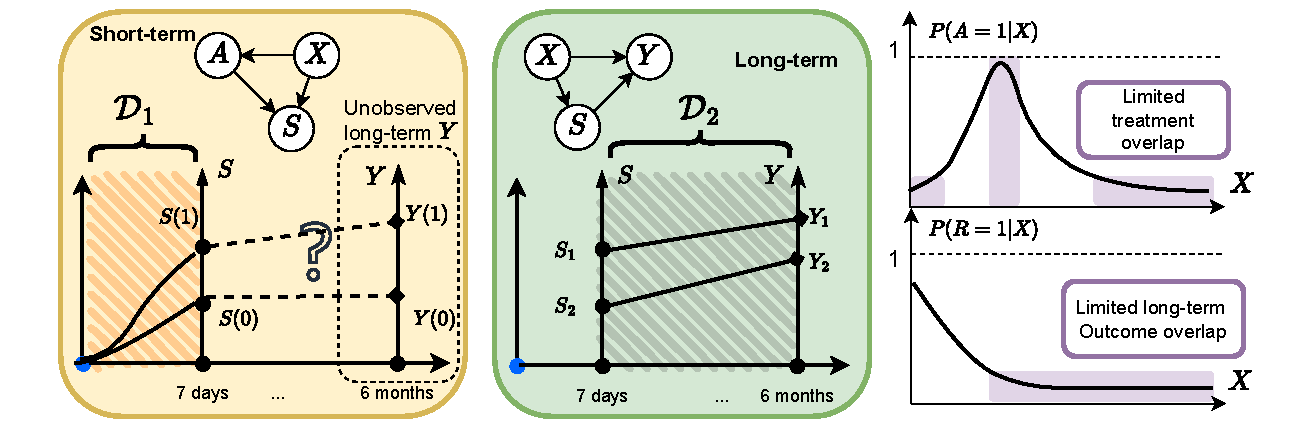
\includegraphics[width=1.0\linewidth]{images/Concept.pdf}
    \caption{\textbf{Our HLTE setting:} The yellow and green box illustrate our two-sample setting. $\mathcal{D}_1$ and $\mathcal{D}_2$ share covariates $X$ and surrogates $S$. The surrogate index (i.e. $\E_{\mathcal{D}_2}[Y|S,X]$), learned in the long-term dataset, is used as a proxy for long-term outcomes in the short-term experiment. The left plot shows the two overlap issues.}
    \label{fig:concept}
    \vspace{-0.5cm}
\end{figure}

In this paper, we address these challenges by proposing the \textbf{\methods} (Long-Term-Orthogonal-Learners), a novel class of orthogonal meta-learners for estimating HLTEs from a short-term randomized dataset $\mathcal{D}_1$ and a long-term observational dataset $\mathcal{D}_2$. The key idea behind our \methods is to explicitly account for both (i)~limited treatment assignment overlap and (ii) limited long-term outcome overlap. To this end, our \methods \textit{retarget} the learning objective through carefully designed overlap weights that downweight samples with weak treatment overlap or low probability of observing long-term outcomes, thereby stabilizing the second-stage learning problem. We show that the retargeted loss is equivalent to the weighted oracle loss. Then, we instantiate three variants: (1)~\textbf{\TO}, (2)~\textbf{\LO}, and (3)~\textbf{\DO} with different weightings tailored for different overlap regimes. We further provide an error bound for the \methods and give the conditions under which a quasi-oracle convergence rate can be achieved. Importantly, our \methods are fully model-agnostic: they can be instantiated with arbitrary machine learning models (e.g., neural networks) for both nuisance estimation and outcome learning, making them broadly applicable in high-dimensional HLTE settings from practice.

%Together, these properties enable reliable and stable estimation of heterogeneous long-term treatment effects even in challenging low-overlap regimes. 

% In this paper, we address this limitation by proposing \textbf{DOWOL} (Dual-Overlap Weighted Orthogonal Learners), a novel class of meta-learners for HLTE estimation from $\mathcal D_1$ and $\mathcal D_2$.  Our method (i) remains Neyman-orthogonal, and therefore robust against nuisance estimation errors; (ii) incorporates dual retargeting that downweights samples with low treatment overlap and low long-term observation overlap, stabilizing the second-stage learning objective; and (iii) are model-agnostic, allowing arbitrary ML models in both nuisance estimation and HLTE learning.

Our \textbf{contributions} are:\footnote{Code is available at \href{https://anonymous.4open.science/r/LT-learner-for-Long-term-HTE-5041}{https://anonymous.4open.science/r/LT-learner-for-Long-term-HTE-5041}. Upon acceptance, we move the code to a public GitHub repository.} (1)~We propose the \textit{\methods}, a novel class of orthogonal meta-learners for estimating HLTEs, which are designed to be robust to different forms of low overlap. (2)~We provide theoretical guarantees on the convergence rate of our \methods. (3)~We conduct extensive experiments on both synthetic and semi-synthetic datasets to demonstrate the robustness of our \methods in low-overlap regimes.

% ; a special case recovers an R-learner analogue for long-term effects.

\vspace{-0.2cm}

\section{Related work}
\label{sec:related_work}



\textbf{Orthogonal learners for heterogeneous treatment effects (HTEs):} Several machine learning methods have been developed for the standard HTE setting with a single dataset \citep[e.g.,][]{Shalit.2017, Curth.2021}, where, unlike our HLTE setting, the outcome of interest is directly available in the randomized (or observational) data. State-of-the-art methods are model-agnostic two-stage estimators, in which nuisance functions are estimated in the first stage and where the target HTE is learned in a second stage function by minimizing an orthogonal loss function \cite{Foster.2023} in the second stage to predict the HTEs. Orthogonality ensures robustness w.r.t. nuisance estimation errors \cite{Chernozhukov.2018} and thus prevents plug-in bias~\cite{Kennedy.2022-Sempiparametric}.
%and often brings other favorable properties such as double robustness or \TODO{shouldN#t we a bit more careful here -- this does not come alawys automatically?}quasi-oracle convergence rate \cite{Foster.2023}. 
Examples include the DR-learner \cite{Kennedy.2020-DR-learner}, and R-learner \cite{Nie.2021}. However, these learners are \textit{not} directly transferable from the HTE to the HLTE setting. 

%\citet{Morzywolek.2023} further propose a general treatment overlap-weighted orthogonal learner. However, these orthogonal learners are \textit{not} tailored for our HLTE setting, where the long-term outcome is \textit{not} available in the dataset. Further, the main source of overlap is different (i.e., treatment overlap vs. long-term outcome overlap, which is unique to our setting). 

% https://pubsonline.informs.org/doi/10.1287/mksc.2022.0379

\textbf{Data combination for causal inference:} A large body of work studies treatment effect estimation by combining multiple datasets, such as combinations of observational datasets~\citep[e.g.,][]{Yang.2020, Yuxin.2025}, combinations of experimental datasets~\citep[e.g.,][]{Debray.2015, Tan.2022, Brantner.2024-comparison}, or mixed combinations of both observational \textit{and} experimental datasets \citep[e.g.,][]{Hatt.2022, Wu.2022-integrative, Brantner.2023, Yao.2024combining, Yuxin.2025, parikh.2025double, Chen.2025, Cai.2025-Individual, Chen.2025-sequential}
, including for both average and heterogeneous treatment effects. For a detailed review, we refer to \citet{Colnet.2024}.
In these settings, the motivation for data combination is typically to leverage complementary information across datasets while assuming that treatment \textit{and} outcomes are observed in \textit{all} datasets. Hence, the works from this stream are different from our paper and \textit{not} applicable. One paper aims to relax the setting by assuming a combination where long-term outcomes are observed in only one dataset while treatments must still be observed in both \cite{Cai.2025-Individual}; however, this is still \textit{different} from our setting, where treatments are observed in only one dataset and long-term outcomes in the other dataset.


\textbf{Average long-term treatment effects (ALTEs):} A related but different setting aims at estimating \textit{average} long-term treatment effects (ALTEs). In this setting, ALTEs are typically identified by mediating the treatment effects via surrogate variables under suitable assumptions \citep[e.g.,][]{Prentice.1989, Frangakis.2002, Lauritzen.2004}. One approach is to build a ``surrogate index'' (i.e., a group of short-term endpoints) as the proxy for long-term outcomes under unconfoundedness \citep{Athey.2025, Chen.2023}. Subsequent works estimate ALTEs with modified settings and assumptions~\citep[e.g.,][]{Athey.2020a, Ghassami.2022, Goffrier.2023, Obradovic.2024,Cai.2024-latent, Imbens.2025}. Other works also study ALTE estimation in the context of policy optimization tasks \citep[e.g.,][]{McDonald.2023, Park.2024bracketing, Yang.2024-Targeting, Yang.2024-LearningTheOptimalPolicy, Wang.2024, Saito.2024LOPE}. However, these works all target the ALTE, which only captures \textit{population-level} effects and which thus \textit{ignores} how long-term treatment effects vary across individuals or subpopulations. %In contrast, we focus on the \textit{heterogeneous} long-term effect, which is the basis for personalized decision-making. 

\textbf{Heterogeneous long-term treatment effects (HLTEs):} There are some works studying HLTEs under alternative problem formulations, such as \textit{dose–response} settings~\citep{Singh.2022, Yang.2025-dose-response}. These approaches focus on \textit{continuous} treatments and rely on different estimation strategies because of which they are \textit{not} applicable to the canonical HLTE setting with binary treatments considered in this paper. \citet{Huang.2024-Doingmore} constructs a noise-reduced surrogate index via separate imputation; however, this requires additional long-term variables other than $Y$ and is thus \emph{not} applicable to our setting. 

 Closest to our work is \citet{Chen.2025}, who proposed a multiply robust (MR) HLTE estimator in the setting of Conditional Additive Equi-Confounding Bias~\citep{Ghassami.2022}. However, it requires observed treatment in both datasets and does not adjust for confounding in the canonical setting with surrogacy assumption. Thus, it is not applicable. Interestingly, there is \emph{no} research that explicitly studies HLTE estimator for the canonical HLTE setting. Nevertheless, such estimators can be readily extended from the literature (we do so in \Cref{sec:standard_learners}). In particular, we formalize several learners with different adjustment strategies that are tailored to the HLTE setting, namely, (1) \textbf{long-term T-learner}, (2)~\textbf{long-term RA-learner}, (3)~\textbf{long-term IPW-learner}. In Section~\ref{subsec:instantiation}, we present the \textbf{\DR} as a special instantiation of our \methods framework. \textit{However}, these aforementioned meta-learners have limitations: The long-term RA-learner is subject to \textit{plug-in bias}~\cite{Kennedy.2022-Sempiparametric}. The long-term IPW-learner suffers from \textit{high finite-sample variance} under low treatment overlap due to divisions by near-zero values. While the DR-learner and the MR estimator from \citet{Chen.2025} mitigates first-order bias from nuisance estimation via Neyman orthogonality, they are \textit{sensitive to (i)~low treatment overlap and (ii)~low long-term outcome overlap in finite samples} (i.e., when outcomes are only sparsely available for certain subgroups). 


%losest to our work is \citet{Chen.2025}, albeit in a different setting\footnote{In \citet{Chen.2025}'s setting, treatment is observed in both datasets.}. The paper proposed the regression-adjustment-based, propensity-based, and multiple robust HLTE meta-learners, which could be viewed as the long-term counterparts to RA-learner, IPW-learner and DR-learner in the standard HTE estimation. In fact, these learners can also be derived for our setting analogously (as we have shown in Section~\ref{sec:formulation}).

%For the binary HLTE setting, existing works can be broadly distinguished by how confounding is adjusted when combining short-term experimental data with long-term observational data.  

%\citet{Cai.2025-Individual} targets long-term individual treatment effects, but relies on an auxiliary heterogeneity variable for identifiability, so it is \emph{not} applicable to our setting. 
%\citet{Chen.2025-sequential} studies HLTE under sequential latent confounding, where treatment is observed in both datasets and the long-term outcome is explicitly modeled as a future time point of the shot-term surrogate trajectory; these requirements fall outside our HLTE setting and hence is also not applicable. Closest to our work is \citet{Chen.2025}, albeit in a different setting\footnote{In \citet{Chen.2025}'s setting, treatment is observed in both datasets.}. The paper proposed the regression-adjustment-based, propensity-based, and multiple robust HLTE meta-learners, which could be viewed as the long-term counterparts to RA-learner, IPW-learner and DR-learner in the standard HTE estimation. In fact, these learners can also be derived for our setting analogously (as we have shown in Section~\ref{sec:formulation}). However, just like the HTE estimators, each HLTE meta-learner above has its limitations: The RA-learner is subject to \textit{plug-in bias}. The IPW-learner suffers from high variance under limited treatment overlap. While the DR-learner mitigates first-order bias from nuisance estimation, it is sensitive to (i)~limited treatment overlap and (ii)~limited outcome overlap in finite samples (i.e., when outcomes are only sparsely available for certain subgroups). 


 


% Both model-based method (learners based on specific machine learning models) and model-agnostic methods are developed for HLTE estimation: (1) Model-based: \cite{Cai.2025-Individual} proposes a latent representation learning-based estimator, instantiated by a variational auto-encoder. \cite{Singh.2022} adapts kernel ridge regression to extrapolate long-term dose-response curves (continuous treatment type). These methods are not model-agnostic nor orthogonal, making them only works when the latent identifiability is satisfied by the data generating model or subject to so-called plug-in bias \cite{Kennedy.2022-Sempiparametric}. (2) Model-agnostic: \cite{Chen.2025} proposes the learner that regresses the influence function-based pseudo-outcomes (analogous to DR-learner in standard HTE estimation). In fact, the Neyman-orthogonal pseudo-outcomes built in previous ALTE methods can be directly brought to estimate the HLTE via a second-stage pseudo-outcome regression. However, these methods are based on efficient influence function and hence are optimized for asymptotic efficiency. Under finite sample, these orthogonal learners are not robust against treatment or observation overlap violations. 

\textbf{Research gap:} Existing methods for HLTE estimation fail to address the challenge due to (i)~limited treatment overlap and (ii)~limited long-term outcome issue in finite samples (see Table~\ref{tab:related-works}). To the best of our knowledge, we are the first to provide a general class of orthogonal learners that is robust in low-overlap regimes. 

\vspace{-0.2cm}

\section{Problem formulation} 
\label{sec:formulation}

\textbf{Setup:} We follow the canonical long-term outcome setting \citet{Athey.2025, Chen.2023}, but adapt it from ALTEs to HLTEs. We thus consider two datasets: a short-term experimental dataset $\mathcal{D}_1$ and a long-term historical observational dataset $\mathcal{D}_2$, with $N_1$ and $N_2$ units respectively.  $\mathcal{D}_1$ and $\mathcal{D}_2$ differ in terms of which variables are observed (see Figure~\ref{fig:concept}). 

Let $A \in \{0,1\}$ be the treatment variable, $X\in \mathcal{X}\subset\mathbb{R}^{d_x}$ be pre-treatment covariates, $S \in \mathcal{S}\subset \mathbb{R}^{d_s}$ be the short-term surrogate variable, $Y\in\mathbb{R}$ be the long-term outcome, and $R \in \{0,1\}$ be the dataset indicator, denoting whether the observation belongs to $\mathcal{D}_1$ ($R=0$) or $\mathcal{D}_2$ ($R=1$).

The covariates $X$ and short-term surrogates $S$ are observed in both $\mathcal{D}_1$ and $\mathcal{D}_2$. The long-term outcome $Y$ is observed only in $\mathcal{D}_2$. The treatment $A$ is only measured in the experimental dataset $\mathcal{D}_1$ but \textit{not} in $\mathcal{D}_2$ (e.g., because this is a new treatment that was not applied previously). Formally, we can combine $\mathcal{D}_1$ and $\mathcal{D}_2$ to build a unified dataset with $N=N_1+N_2$ units:
$%\begin{align*}
    \mathcal{D}=\mathcal{D}_1 \cup \mathcal{D}_2=\{(X_i, (1 - R_i)A_i, S_i, R_i, R_iY_i)\}_{i=1}^N$.
%\end{align*}

\textbf{Nuisance functions:} Our method relies on a set of nuisance functions. % which are auxiliary quantities that are not of direct interest but are required to characterize the data-generating process and construct the final estimator In the case of our \methods, these are:

\vspace{-0.5cm}
\footnotesize
\begin{align}
    &\pi_s(s,x)=\Pr(A=1\mid S = s,X = x,R = 0),\label{pi-sx-def}\\
    &\pi(x)=\Pr(A=1\mid X = x,R = 0),\label{pi-x-def}\\
    &\rho_s(s,x)=\Pr(R=1\mid S = s,X = x), \label{rho-sx-def}\\
    &\rho(x)=\Pr(R=1\mid X = x), \label{rho-x-def}\\
    &h(s,x)=\mathbb E[Y\mid S = s,X = x,R = 1], \label{h-def}\\
    &\mu(a,x)=\mathbb E \big[h(S,X)\mid A = a,X = x,R = 0\big] \label{mu-def}.
\end{align}
\vspace{-0.5cm}
\normalsize

We let $\eta$ denote the complete set of nuisance functions, i.e.,
\begin{equation}
\label{eq:def-eta}
    \eta = (\pi(x), \pi_s(s,x), \rho(x),\rho_s(s,x),h(s,x), \mu(a,x)).
\end{equation}
\textbf{Causal estimand:} We build upon the potential outcome framework~\cite{Rubin.1972} and aim to estimate the HLTE in the experimental dataset, given by
\begin{align}
\label{tau0-def}
    \tau^0(x)=\E\left[Y(1)-Y(0) \mid X=x,R=0\right].
\end{align}
This estimand captures how long-term treatment effects vary at the individual or subgroup level as a function of covariates $X$, thus allowing for fine-grained heterogeneity in long-term responses to inform personalized decision-making. In contrast, population-level estimands such as the ALTE as in \citet{Athey.2025} target average effects across the entire population and do not characterize which individuals or subpopulations benefit most from the treatment.

%In Appendix \TODO{XXX}, \TODO{we also provide  an extension for HLTEs estimation in the observational dataset}. This extension is relevant in settings where interest lies in characterizing HLTE within the population represented by the observational data rather than the experimental sample, for example, to assess the efficacy in routine care or to account for differences in the prevalence of vulnerable subpopulations that may be underrepresented in clinical trials \citep{Feuerriegel.2024}.

\textbf{Identifiability: } We use the following standard assumptions from~\citet{Athey.2025} to ensure the identification. % of $\tau^0(x)$. 
\begin{assumption}[Consistency]
\label{assumption-consistency} \emph{For all $a \in \{0,1\}$, we have $S(a)=S, \,Y(a)=Y$ whenever $A=a$.}
\end{assumption}
\begin{assumption}[Positivity] 
\label{assumption-positivity} \textit{The treatment overlap is nondegenerate: $0< P(A=1 \mid X=x, R=0)<1, \; \forall x\in \mathcal{X}$.}
\end{assumption}

\begin{assumption}[$\mathcal{D}_1$ unconfoundedness]
\label{assumption-unconf} \emph{For all $a \in \{0,1\}$, we have} $A \indep S(a), Y(a) \mid X, R=0$.
\end{assumption}

\begin{assumption}[Surrogacy~\cite{Prentice.1989}]
\label{assumption-surrogacy} \emph{The long-term effect is fully mediated by the surrogate variable in $\mathcal{D}_1$:} $A \indep Y \mid S, X,R=0$ and $0 < P(R=1 \mid S=s,X=x) < 1$.
\end{assumption}
\begin{assumption}[Long-term outcome comparability]
\label{assumption-compara} \emph{The distribution of $Y$ is invariant to whether it belongs to $\mathcal{D}_1$ or $\mathcal{D}_2$:} $R \indep Y \mid S, X$.
\end{assumption}
Assumptions~\ref{assumption-consistency}, \ref{assumption-positivity}, \ref{assumption-unconf} are standard in the observational causal inference literature~\cite{Rubin.1974, Imbens.1994, Kallus.2025, Athey.2025}. Assumption~\ref{assumption-surrogacy} is a necessary modeling assumption for long-term inference and is widely adopted in prior literature~\citep{Athey.2025, Chen.2023, Yang.2024-Targeting, Kallus.2025}.\footnote{In principle, low-dimensional surrogate variables may not fully mediate long-term treatment effects in all settings~\citep{Freedman.1992}; however, in many contemporary applications, this issue is naturally addressed by incorporating rich collections of surrogate measures. This is common in medical settings such as intensive care units (ICUs) or oncology, where high-frequency and multi-modal data---including vital signs, laboratory measurements, and imaging---provide informative surrogates for long-term clinical outcomes.} Assumption~\ref{assumption-compara} requires that the conditional distribution of $Y$ given $(S,X)$ is transportable between $\mathcal{D}_1$ and $\mathcal{D}_2$, which is a mild assumption that is common in most data combination tasks~\cite{Athey.2025, Chen.2023, Yang.2024-Targeting}. When all the above assumptions are satisfied, we call the problem the \emph{standard surrogacy model}~\cite{Chen.2023}. 

We can then identify the HLTEs via:

\vspace{-0.5cm}
\footnotesize
\begin{align}
    \label{eq:identification-tau0}
    \hspace{-0.4cm}
    \tau^0(x)=\mathbb{E}[Y^1-Y^0 \mid X=x,R=0]=\mu(1,x)-\mu(0,x).
    \hspace{-0.1cm}
\end{align}
\vspace{-0.5cm}
\normalsize


A formal proof of Eq.~(\ref{eq:identification-tau0}) is provided in Appendix~\ref{app:identification}. %The identification of the average treatment effects is shown in~\cite{Athey.2025}. Here we adopt the same setting and then extend the results to the heterogeneous effects.

%\textbf{Disadventage of plug-in estimators: } Given the identification in Eq.~\ref{eq:identification-tau0}, a direct way to achieve HLTEs is to estimate the nuisance functions $h(s,x)$ and then $\mu(a,x)$. However, \TODO{Explain plug-in bias induced by nuisance estimation + inductive bias}. These plug-in estimators are called T-learner~\cite{Curth.2021}.

\section{T-, RA-, and IPW-learners for HLTE estimation}
\label{sec:standard_learners}

\begin{table}

\centering
\tiny
\caption{\textbf{Overview of meta-learners for HLTE estimation.} Our \methods are the only approaches that are both Neyman-orthogonal and robust to different types of low-overlap scenarios.}
\label{tab:related-works}
\resizebox{0.5\textwidth}{!}{%
  \begin{tabular}{ll
      >{\columncolor{shallowyellow}}c
      @{\hspace{10pt}}
      >{\columncolor{shallowblue}}c
      >{\columncolor{shallowblue}}c
  }
\toprule
\textbf{Method}
& \makecell{\textbf{Analogy in }\\\textbf{standard HTE setting}}
& \makecell{\textbf{Neyman}\\\textbf{orthogonal}}
& \makecell{\textbf{Robust to low} \\ \textbf{treatment overlap}} 
& \makecell{\textbf{Robust to low} \\ \textbf{outcome overlap}} \\
\midrule
\LTT
& T-learner~\citep{Kunzel.2019} & \xmark & \xmark & \xmark \\
\LTRA
& RA-learner~\citep{Curth.2021} & \xmark & \xmark & \xmark \\
\LTIPW
& IPW-learner~\citep{Curth.2021} & \xmark & \xmark & \xmark \\
\textbf{\DR (\emph{ours})}
& DR-learner~\citep{Kennedy.2020-DR-learner} & \cmark & \xmark & \xmark \\
\textbf{\TO (\emph{ours})} & R-learner~\citep{Nie.2021} & \cmark & \cmark & \xmark \\
\textbf{\LO (\emph{ours})} & -- & \cmark & \xmark & \cmark \\
\textbf{\DO (\emph{ours})} & -- & \cmark & \cmark & \cmark \\
\bottomrule
\end{tabular}
}
\vspace{-0.3cm}
\end{table}

%In this section, we briefly give the background of two-stage estimators

In this section, we briefly introduce how the T-, RA-, and IPW-learners for the standard HTE estimation setting\footnote{This refers to the setting where there is only a single dataset that contains fully observed $(X,A,Y)$ with no unobserved confounding~\cite{Kunzel.2019}.} can be adapted to the HLTE setting (see Table~\ref{tab:related-works}). Since the long-term outcome $Y$ is unobserved in $\mathcal{D}_1$, we must bridge the gap between short term surrogates $S$ and $Y$. To do this, we learn $h(s,x) = \E[Y \mid S=s, X=x, R=1]$ from $\mathcal{D}_2$ and evaluate it on $\mathcal{D}_1$. Under the surrogacy assumption (Assumption~\ref{assumption-surrogacy}) and the comparability assumption (Assumption~\ref{assumption-compara}), $h$ is an unbiased proxy of the unobserved $Y$ in $\mathcal{D}_1$\footnote{\citet{Athey.2025} refers to $h$ as the surrogate index}. As a result, we can simply replace $Y$ by $h(S,X)$ in the standard HTE estimators to construct the analogous HLTE learners. While new in our setting, these learners serve as natural baselines and provide useful intuition for the challenges of HLTE estimation, and thus motivate our \methods. We summarize these learners in Table~\ref{tab:related-works}.

$\bullet$\,\textbf{Long-term T-learner (\LTT):} The simplest approach is to estimate the conditional response functions $\mu_a(x)=\E\left[h(S,x)|A=a, X=x,R=0\right], \;a\in\{0,1\}$. Then, we obtain the \emph{plug-in} HLTE estimator: $\hat\tau^0_{T}(x)=\hat\mu_1(x) - \hat\mu_0(x)$. We name it the long-term T-learner following the standard HTE setting~\cite{Kunzel.2019}. This T-learner plugs-in the estimated $\hat\mu$ directly into the identification in Eq.~(\ref{eq:identification-tau0}). However, this induces the so-called "plug-in bias"~\citep{Kennedy.2022-Sempiparametric}, which means that the estimator inherits the entire estimation error of the nuisance functions $\hat\mu_1$. 
%However, studies have shown that $\hat{\tau}^0$ is often simpler than $\mu_a$, fitting two separate potential outcome estimators may lead to overfitting and bring \emph{inductive bias} to the estimate of $\tau^0$\cite{Curth.2021-inductive}.

To mitigate the plug-in bias in standard HTE estimation, literature often employs two-stage learners that regress a constructed pseudo-outcome on covariates~\cite{Kunzel.2019, Curth.2021}. Here, we formulate the long-term analogues of these learners as follows:

$\bullet$\,\textbf{Long-term RA-learner (\LTRA):} The RA-learner follows a two-stage pseudo-outcome regression. It fits estimates $(\hat{h}, \hat\mu_1, \hat\mu_0)$ in the first stage. In the second stage, it regresses the regression-adjusted pseudo-outcome on $\mathcal{D}_1$:
%\footnotesize
%\begin{align}
\begin{align}
\label{ra-loss}
    \mathcal{L}_{\mathrm{RA}}=\E\left[\1(R=0)(\mathcal{T}_\mathrm{RA} - g(X))^2\right], 
\end{align}
where $\mathcal{T}_\mathrm{RA}= A(\hat{h}(S,X)-\hat\mu_0(X)) + (1-A)(\hat\mu_1(X)-\hat{h}(S,X)).$
%\notag
%\end{align}
%\normalsize

$\bullet$ \,\textbf{Long-term IPW-learner (\LTIPW):} The IPW-learner uses inverse-propensity-based pseudo-outcome:
$\mathcal{T}_\mathrm{IPW} = \left(\frac{A}{\hat\pi(X)}-\frac{1-A}{1-\hat\pi(X)}\right) \hat{h}(S,X)$, and the second stage loss is defined as:
\begin{align}
\label{ipw-loss}
    \mathcal{L}_{\mathrm{IPW}}=\E\left[\1(R=0)(\mathcal{T}_\mathrm{IPW} - g(X))^2\right]
\end{align}
However, $\mathcal{T}_\mathrm{IPW}$ contains terms like $\frac{1}{\hat\pi(X)}$ (or $\frac{1}{1-\hat\pi(X)}$), which is highly unstable in limited treatment overlap regimes. 

\textbf{Why do we need orthogonal learners:}
Although with a two-stage framework, the \LTRA and \LTIPW still have two limitations: (i) the second-stage loss only uses data from $\mathcal{D}_1$, and (ii) they are still sensitive to the nuisance estimation errors $\hat\eta-\eta$. To overcome these limitations, current state-of-the-art two-stage methods for treatment effect estimation (either standard or long-term) use the so-called \emph{orthogonal learners}~\cite{Chernozhukov.2018, Foster.2023}. A learner with loss function $\mathcal{L}(g, \eta)$ is defined as orthogonal if the Gateaux derivative of the loss w.r.t. the nuisance parameters vanishes at the truth:
\begin{align}
    D_\eta D_g \mathcal{L}(g, \eta)[\hat{g}-g, \hat\eta - \eta] = 0. 
\end{align}
Intuitively, orthogonality ensures that the gradient of the loss function is insensitive to perturbations in the nuisance parameters~\cite{Chernozhukov.2018}. This allows faster convergence of the target estimator even with a slow convergence of the nuisances. Furthermore, orthogonal loss typically utilizes the full population, instead of a conditional population as in Eq.~(\ref{ipw-loss}), Eq.~(\ref{ra-loss}). In the section below, we propose our \methods, a class of orthogonal learners for HLTE estimation, which are designed to be robust against nuisance errors and stable in low-overlap regimes.



%The learners discussed above are all sensitive to the nuisance estimation errors $\hat\eta-\eta$. The underlying reason is that they are not Neyman-orthogonal (i.e. $\E[D_\eta\mathcal{T}(Z;\eta)]\neq 0$), and thus any error from $\hat\eta$ will have a first-order impact on the pseudo-outcome~\cite{Chernozhukov.2018}. 


%$\bullet$\,\textbf{DR-learner:} To mitigate this limitation, the DR-learner constructs a pseudo-outcome based on the \textit{efficient influence function} (EIF). %While it follows a similar two-stage learning procedure as the RA- and IPW-learners,
% (1)~\textit{First stage:} Estimate the nuisance functions $\eta$ (see Eq.~\ref{eq:def-eta}) from the data. (2)~ \textit{Second stage:} Learn the target function by minimizing a loss function $\hat{\tau}=\argmin_{g \in \mathcal{G}}\mathcal{L}(g;\hat\eta)$, 
%its major benefit is that it allows the construction of \emph{orthogonal learners}~\cite{Foster.2023}. This means that 
%Due to orthogonality, the (functional) derivative of the loss function is robust against misspecification of the nuisance estimators~\cite{Chernozhukov.2018}:
%
%\begin{align}
%\label{orthogonality-def}
%\end{align}
%Under certain assumptions, this brings favorable properties such as a faster convergence of the target even with a slow convergence of the nuisances. 





%In the following section, we address the low overlap issue by developing a weighted, Neyman-orthogonal learner.

\section{Our \methods}
\label{sec:method}

\textbf{Main idea of our \methods:} Existing studies have shown that, orthogonal learners without sample reweighting are usually hurt by low-overlaps under finite samples~\cite{Fisher.2023, Frauen.2025-model, Frauen.2025-survival} (See Appendix~\ref{app:variance} for the variance analysis of the unweighted \DR). Our goal is to design learners that are both orthogonal and robust against low-overlap regimes. To do this, the key idea is to downweight the samples with (i)~low treatment or (ii)~low long-term outcome overlap. %This reweighting strategy is widely used in HTE estimation to stabilize the learner~\cite{Fisher.2023, Frauen.2025-model, Frauen.2025-survival}. 
Conceptually, this corresponds to optimizing a weighted oracle risk of the form
\begin{equation*}
%\label{eq:oracle-omega-weighted-loss}
\mathcal{L}_\omega^{\text{oracle}}(g)=\mathbb{E}\bigl[\omega(\pi(X), \rho(X))\cdot(\tau^0(X)-g(X))^2 \mid R = 0\bigr],
\end{equation*}
where $\omega(\pi(X), \rho(X))>0$ represents a \textit{weighting function} that \textit{retargets} the objective to downweight the samples with low overlap while preserving the target HLTE $\tau^0(x)$. A simple example of such a weighting function is
\begin{align}
\label{example-omega}
    \omega(\pi(x),\rho(x))=\underbrace{\pi(x)(1-\pi(x))}_{\text{treat. overlap}} \cdot\underbrace{\rho(x)}_{\text{long-term outcome overlap}}
\hspace{-0.3cm}
\end{align}
The loss $\mathcal{L}_\omega^{\text{oracle}}$ is an oracle objective because it depends on the true HLTE $\tau^0(x)$, which is our target estimand and thus unobserved in practice. Hence, our goal is to construct a loss function $\mathcal{L}_\omega(g;\eta)$ that is equivalent to this oracle objective and can be optimized using observed data. This requires a non-trivial derivation to ensure that the resulting loss (i) shares the same minimizer as the oracle loss and (ii)~is Neyman-orthogonal w.r.t. the nuisance functions.


\textbf{Overview:} In Section~\ref{subsec:ortho-weight-loss}, we show how we orthogonalize the oracle weighted loss. In Section~\ref{subsec:estimating-hlte}, we give the algorithm for training the HLTE estimator. Then, in Section~\ref{subsec:instantiation}, we give specific instantiations of our \methods for different types of low-overlap regimes. Finally, in Section~\ref{subsec:convergence}, we show that the estimator achieves quasi-oracle convergence rate under mild conditions.

\subsection{Orthogonalizing the weighted oracle loss}
\label{subsec:ortho-weight-loss}

In this section, we derive the orthogonal loss that has the same minimizer as the weighted oracle loss, under true nuisance $\eta$ and model class $\mathcal{G}$. Following a similar approach as in~\cite{Morzywolek.2023}, we start by deriving the EIF for the \emph{$\omega$-weighted} average effect, which is defined as:
\begin{equation}
\vspace{-0.1cm}
\label{eq:walte-def}
    \tau^0_\omega =\frac{\E\left[\omega(X)\tau^0(X)\mid R=0\right]}{\E\left[\omega(X)\mid R=0\right]}:= \frac{N_\omega}{D_\omega}.
\end{equation}
Here, for simplicity, we denote $\omega(x)=\omega(\pi(x),\rho(x))$. The basic ideas behind are: (1)~If $\mathcal{G}$ is a class of constant function, then $g^*(x) \equiv \tau^0_\omega$ is the minimizer of $\mathcal{L}_\omega^{\text{oracle}}(g)$. (2)~The Gateaux derivative of the EIF w.r.t. the nuisance functions $\eta$ is zero~\cite{Chernozhukov.2018}. Thus, EIF-based pseudo-outcomes often satisfy Neyman-orthogonality and have conditional mean $\E[Y(1)-Y(0)\mid X,R=0]$, such as the DR-pseudo-outcome~\cite{Kennedy.2020-DR-learner}.\footnote{See Appendix~\ref{app:theory} for a theoretical background.} See Appendix~\ref{app:EIF-weighted-ATE} for the EIF.


\begin{contributionbox}
\textbf{LT-O-learners:} Let $Z$ be $(X,A,S)$ when $R=0$ and $(X, S, Y)$ when $R=1$. Based on the derived EIF, we propose our orthogonal loss as follows:
\begin{equation}
\label{eq:weighted-ortho-loss-tau0}
\mathcal{L}_\omega(g, \eta) = \mathbb{E} \left[ \omega^*(Z;\eta) g(X)^2 -2\mathcal{T}_{LT}\cdot g(X)\right],
\end{equation}
where $\omega^*$ is the \textit{LT weighting function} defined as:
\footnotesize
\begin{align}
    \omega^*(Z;\eta) &= \1(R=0) \omega(X) + \Omega(Z;\eta) \label{omega-star-def} \\
    \Omega(Z;\eta)&=\1(R=0)\frac{\partial \omega}{\partial \pi} (A - \pi)
    + (1-\rho) \frac{\partial \omega}{\partial \rho} (R - \rho), \notag
\end{align}
\normalsize
and the \textit{LT pseudo-outcome} $\mathcal{T}_\mathrm{LT}(Z;\eta)$ is
\footnotesize
\begin{align}
\label{Tau-LT-def}
    \mathcal{T}_\mathrm{LT}&(Z;\eta) =  \1(R=0) \omega(X) \hat{\tau}_\mathrm{AIPW}(Z;\eta)\\
     +  \1(R=1)& \cdot\omega(X) \psi_\mathrm{obs}(Z;\eta) + (\mu(1,X)-\mu(0,X)) \Omega(Z;\eta),\notag
\end{align}
with
\begin{align*}
    \hat{\tau}_\mathrm{AIPW}&(Z;\eta) = \mu(1,X) - \mu(0,X) %\label{tau-AIPW-def}
    \\ 
    &\quad\qquad +\frac{A-\pi(X)}{\pi(X)(1-\pi(X))}(h(S,X) - \mu(A,X)) , \notag \\
    \psi_\mathrm{obs} =& \frac{1-\rho_s(S,X)}{\rho_s(S,X)} \left( \frac{\pi_s(S,X) - \pi(X)}{\pi(X)(1-\pi(X))} \right)
    \cdot\big( Y - h(S,X) \big) \label{psi-obs-def}
\end{align*}

\end{contributionbox}
\normalsize
Intuitively, $\omega^*$ consists of a main part $\omega(x)$ and a residual-based $\Omega(Z;\eta)$\footnote{$\Omega(Z;\eta)$ can be viewed as a mean $0$ term that corrects the first-order bias of the weight estimator $\hat\omega(X)=\omega(\hat\pi(X),\hat\rho(X))$.} and thus $\omega^*\approx \omega$ on average when $R=0$. Take $\omega=\pi(1-\pi)\rho$ as an example: When either 1) treatment overlap is low (small $\pi(1-\pi)$) or 2) long-term outcome overlap is low (small $\rho$), the sample is downweighted in the pseudo-outcome regression in Eq.~(\ref{eq:weighted-ortho-loss-tau0}) via $\omega^*\approx \omega$. In fact, we have the following (see Appendix~\ref{app:proofs} for detailed proofs):
%An advantage of our \methods is that users can customize $\omega(x)$ as long as it effectively downweights the sample with low overlap.
%The following remark shows that we are indeed optimizing the weighted oracle target loss $\mathcal{L}_\omega^{\text{oracle}}$ (see Appendix~\ref{app:proofs} for details). 
%Note that $\E\left[\Omega(Z;\eta) \mid X\right] = 0$, and $\mathcal{T}_\mathrm{LT}(Z;\eta)$ = $\frac{1}{\omega^*(Z;\eta)}$ $\left[\omega(X)\mathcal{T}_\mathrm{DR}+(\mu(1,X)-\mu(0,X)) \Omega(Z;\eta)\right]$. Thus, we have:
\begin{align}
    \E&\left[\omega^*(Z;\eta)\mid X\right] = (1-\rho(X))\omega(X) , \notag \\
    \E&\left[\mathcal{T}_\mathrm{LT}(Z;\eta) \mid X\right] = (1-\rho(X))\omega(X) \tau^0(X).  \notag
\end{align}
Hence, when we optimize $\mathcal{L}_\omega(g, \eta)$, we are always solving for $g^*(X)=\E\left[\mathcal{T}_{LT} \mid X\right] / \E\left[\omega^*\mid X\right]=\tau^0(X), \; \forall X\in \mathcal{X}$ regardless of the weighting function. 


Below, we show that the proposed loss function $\mathcal{L}_\omega(g, \eta)$ satisfies two crucial properties: (1) Neyman-orthogonality, and (2) equivalence with the oracle loss $\mathcal{L}_\omega^{\text{oracle}}(g)$.

\begin{theorem}[Neyman-orthogonality]
    \label{thm:orthogonality}
    The proposed loss $\mathcal{L}_\omega(g, \eta)$ is orthogonal w.r.t. the nuisance $\eta$.
    \vspace{-0.1cm}
\end{theorem}
\begin{proof}
    See Appendix~\ref{app:proofs}.
\end{proof}
Theorem~\ref{thm:orthogonality} establishes that the functional derivative of $\mathcal{L}_\omega(g, \eta)$ is Neyman-orthogonal w.r.t. the nuisance $\eta$, i.e. $D_\eta D_g \mathcal{L}_\omega(g, \eta)[\hat{g}-g, \hat\eta - \eta] = 0.$ This means, nuisance estimation error $\delta_\eta=\hat\eta-\eta$ only has second-order impact on the gradient, which makes the learner robust against misspecification.

\begin{theorem}[Oracle equivalence]
    \label{thm:equiv-loss}
    The minimizer of the loss $\mathcal{L}_\omega(g, \eta)$ within a functional space $\mathcal{G}$ is also the minimizer of the oracle weighted loss, namely:
    \begin{equation}
        \argmin_{g\in \mathcal{G}} \mathcal{L}_\omega(g, \eta) = \argmin_{g \in \mathcal{G}} \mathcal{L}_\omega^{\mathrm{oracle}}(g).
    \end{equation}
    A direct implication is that, if $\tau^0(\cdot)\in \mathcal{G}$, then minimizing our orthogonal loss $\mathcal{L}_\omega(g, \eta)$ yields the true HLTE estimator.
\end{theorem}
\begin{proof}
    See Appendix~\ref{app:proofs}.
\end{proof}

%From theorem~\ref{thm:orthogonality} and theorem~\ref{thm:equiv-loss}, we can see that $\mathcal{L}_\omega(g, \eta)$ is indeed the loss we are trying to find. 

\subsection{Algorithm}
\label{subsec:estimating-hlte}

Based on the proposed loss function in Eq.~(\ref{eq:weighted-ortho-loss-tau0}), we estimate the HLTE following a two-stage procedure (described below), which uses a \emph{sample-splitting}~\cite{Chernozhukov.2018, Kennedy.2023, Morzywolek.2023, Foster.2023}. %Sample-splitting ensures that the parameters of the nuisance models $\hat\eta$ are independent of the data used to estimate the target $g$. The nuisance estimators can thus be treated as fixed functions in the second stage, allowing us to achieve tight error bounds (see Section~\ref{subsec:convergence}). 
Specifically, we randomly split the samples from $\mathcal{D}=\{Z_i\}_{i=1}^{N}$ into two disjoint parts $\mathcal{D}=\mathcal{D}_A \cup \mathcal{D}_B$, with $|\mathcal{D}_A|=N-n, |\mathcal{D}_B|=n$. Then, our \methods proceed as follows

\textbf{Stage \circlednumblue{1}:} We fit the nuisance functions on $\mathcal{D}_A$ data with arbitrary machine learning models to obtain the nuisance estimators $\hat\eta=(\hat\pi, \hat\pi_s,\hat\rho,\hat\rho_s, \hat{h}, \hat\mu)$. %In stage 2, we calculate the estimated weighting function

\textbf{Stage \circlednumblue{2}:} We calculate the estimated LT weighting function and pseudo outcome with the estimated nuisance function in stage 1 on $\mathcal{D}_B$: For $i=1, \ldots ,n$, we compute
\begin{align}
\label{eq:plug-in-nuisance-estimates}
    \hat\omega^*_i=\omega^*(Z_i;\hat\eta), \;\;\; \hat{\mathcal{T}}_i=\mathcal{T}_\mathrm{LT}(Z_i;\hat\eta).
\end{align}
Then, using the nuisance estimates in Eq.~(\ref{eq:plug-in-nuisance-estimates}), we can solve the HLTE estimator by minimizing the empirical loss via
\begin{align}
\label{eq:empirical-loss}
    \hat{g}=\argmin_{g\in\mathcal{G}} \sum_{i=1}^n \hat\omega^*_i g(X_i)^2- 2\hat{\mathcal{T}}_i g(X_i) .
\end{align}

\textbf{Note:} In practice, we implement the two-stage learner with cross-fitting~\cite{Chernozhukov.2018}, instead of the two-samples-splitting strategy. This means we split data into $K$ folds (e.g., $K=5$) and then repeat the procedure above $K$ times: In each iteration, we select one of the $K$ folds as $\mathcal{D}_B$ and treat all the remaining $K-1$ folds as $\mathcal{D}_A$. The final estimator is then the average of the $K$ estimators obtained from each fold.


\subsection{Instantiations}
\label{subsec:instantiation}

Our \methods allow customized weighting functions $\omega(\pi(x),\rho(x))$ to explicitly account for different forms of overlap limitations, including (i)~treatment overlap and (ii)~long-term outcome overlap. Below, we present instantiations tailored to common overlap scenarios.


%In the DR-learner, orthogonality is achieved by constructing a pseudo-outcome based on the EIF (here we use the EIF derived in \citet{Athey.2025, Chen.2023}) for which the conditional expectation equals the HLTE. The second-stage learning problem then reduces to regressing this pseudo-outcome on covariates. 

%In the long-term setting considered here, the corresponding DR pseudo-outcome combines information from both the short-term experimental data and the long-term observational data, as formalized below.

%A popular example is pseudo-outcome regression (POR), where a pseudo-outcome is created and then served as the regression target~\cite{Rubin.2005, Kunzel.2019}. Here, a pseudo-outcome is a random variable constructed via the nuisance functions that tries to approximate $Y(1)-Y(0)$. To make the POR orthogonal, the pseudo-outcome is derived from the EIF of the ALTE. We call this learner the long-term DR-learner, as it is essentially the same as the DR-learner for standard HTE estimation. 

$\bullet$\,\textbf{\DR: } When we trivially set $\omega\equiv1$, i.e. no overlap (NO) weighting in the loss, the learner uses efficient influence function of the ALTE from \citet{Chen.2023, Athey.2025}. As a result, we obtain the \DR under the standard surrogacy model. Substituting $\omega\equiv1$ into Eq.~(\ref{eq:weighted-ortho-loss-tau0}) and Eq.~(\ref{Tau-LT-def}), we achieve the loss as follow:

\footnotesize
\vspace{-0.5cm}
\begin{align}
    \mathcal{L}_1(g, \eta) &= \mathbb{E} \left[ \1(R=0)g(X)^2 -2\mathcal{T}_{DR}\cdot g(X)\right], \\
    \mathcal{T}_\mathrm{DR}(Z;\eta) & =\1(R=0) \hat{\tau}_\mathrm{AIPW}(Z;\eta) + \1(R=1)\psi_\mathrm{obs}(Z;\eta)  \label{DR-pseudo-outcome},
\end{align}
\vspace{-0.5cm}
\normalsize

%
%Here,  $\hat{\tau}_\mathrm{AIPW}(Z;\eta)$ is the standard form of the augmented inverse propensity weighting (AIPW) pseudo-outcome, which is standard in the classical HTE estimation setting except that $Y$ is replaced by the surrogate index $h(S,X)$ since $Y$ is not observed when $R=1$. Then, the pseudo-outcome $\psi_\mathrm{obs}$ corrects the first-order error of the nuisance $h(\cdot,\cdot)$ using the observed long-term outcome $Y$ in $\mathcal{D}_2$. This pseudo-outcome is immediately available from the EIF given in \cite{Athey.2025, Chen.2023}, but adapted from the ALTE to the HLTE setting.
%
%\begin{definition}[Long-term DR-learner]
%\emph{We refer to the estimator $\hat\tau^0_\mathrm{DR}(x) \in \mathcal{G}$ that minimizes the following loss function as the DR-learner:
%    \begin{equation}
        %$\mathcal{L}_\mathrm{DR}(g;\eta)=\E_n\left[(g(X)-\mathcal{T}_\mathrm{DR})^2\right], \; g \in \mathcal{G} $.
%    \end{equation}
%Here, $\mathcal{G}$ is a model class (e.g., linear regression models).}
%\end{definition}
%The DR-learner usually performs better than plug-in learners because the loss function is {orthogonal}.  This was shown previously for other settings, such as the standard HTE setting \cite{Kennedy.2022-Sempiparametric, Foster.2023}. % and in data combination settings where treatments are available in both datasets \cite{Chen.2025}.

%showed that the long-term DR-learner under the Equi-Confounding bias assumption outperforms RA-/IPW-learner. 


\emph{Problems of the \DR:} Although orthogonal, the \DR does not apply any sample-weighting strategy, which leads to large finite-sample variance~\cite{Fisher.2023}. To show this limitation, we analyze the variance of pseudo-outcome $ \mathcal{T}_\mathrm{DR}$ and explain why it has high variance when there is low overlap in Appendix~\ref{app:variance}. As a result, the \DR is not robust to low overlaps.



$\bullet$\,\textbf{\TO:} This variant is designed for when only treatment overlap (TO) is problematic (e.g., because $\mathcal{D}_1$ is small or high-dimensional, so that some subgroups have a low propensity score). We choose the weighting function $\omega(x)=\pi(x)(1-\pi(x))$, which downweights samples with limited treatment overlap. 

Under this choice, the corresponding long-term weighting function simplifies to $\omega^*=\1(R=0)(A-\pi(X))^2$. As a result, the second-stage objective reduces to a special case that is equivalent to an R-learner-style objective~\cite{Nie.2021} but adapted to the long-term setting (see Appendix~\ref{app:TO-LT-learner} for details):

\vspace{-0.5cm}
\footnotesize
\begin{align}
\label{t-learner-loss}
 & \mathcal{L}_{\pi(1-\pi)}(g;\eta)=\mathbb{E}\Bigl[ \1(R=0)\bigl((h(S,X)-m(X))- \\
& -(A -\pi(X))g(X)\bigr)^2 - 2\1(R=1)\psi_{t}(Z;\eta)\,g(X)\Bigr] \notag ,
\end{align}
\vspace{-0.5cm}
\normalsize

where $m(X)=\E\left[h(S,X) \mid X,R=0\right]$, and $ \psi_{t}(Z;\eta)= \frac{1-\rho_s}{\rho_s} \bigl(\pi_s-\pi\bigr)(Y-h).$

%Here, the term involving $\1(R=0)$ corresponds to an R-learner-style objective, where $m(X)=\E\left[h(S,X) \mid X,R=0\right]$ denotes the conditional mean of the surrogate index. Therefore, the TO-LT-learner does not require separate estimation of $\mu_1,\mu_0$, but only the conditional mean function $m$ (analogous to the R-learner for the standard HTE setting~\cite{Nie.2021}).

$\bullet$\,\textbf{\LO: } This learner is intended for settings where only long-term outcome overlap (LO) is low. In this case, we choose the weighting function $\omega(x)=\rho(x)$ to downweight samples with a low probability of observing long-term outcomes. Then, the corresponding LT weighting function and the LT-pseudo-outcome can be computed via

\vspace{-0.5cm}
\footnotesize
\begin{align*}
%\label{o-learner-inst}
\omega^* &= (R-\rho(X))^2,\\
    \mathcal{T}_\mathrm{LT}&= (R-\rho(X))^2 (\mu_1(x) - \mu_0(x)) \\
    +& \begin{cases} 
     \rho(x)\frac{A-\pi(X)}{\pi(X)(1-\pi(X))}(h(S,X) - \mu(A,X)) & \text{if } R=0,\\
     \rho(X)\psi_\mathrm{obs}(Z;\eta) , & \text{if } R=1 .
   \end{cases}
\end{align*}
\normalsize
$\bullet$\,\textbf{\DO:} Finally, we present an instantiation of our estimator for settings in which both treatment overlap and long-term outcome overlap are low. Here, we choose the weighting function $\omega(x)=\pi(x)(1-\pi(x))\rho(x)$, which jointly downweights samples with weak treatment overlap and low probability of observing long-term outcomes. The resulting LT weights and LT pseudo-outcomes are given by

\vspace{-0.5cm}
\footnotesize
\begin{align*}
%\label{hlte-learner-mixed}
    \omega^*(Z;\eta) &= \begin{cases} 
      \rho \big[ \rho\pi(1-\pi) + (1-2\pi)(A-\pi) \big] , & \text{if } R=0 , \\
      \pi(1-\pi)(1-\rho)^2 , & \text{if } R=1 ,
   \end{cases} \\
    \mathcal{T}_\mathrm{LT}(Z;\eta) &= (\mu(1,X)-\mu(0,X))\omega^*(Z;\eta) \notag \\
    &+ \begin{cases} 
     \rho(A-\pi)\big( h(S,X) - \mu(A,X) \big) , & \text{if } R=0 , \\
      \rho \pi(1-\pi) \psi_\mathrm{obs}(Z;\eta) , & \text{if } R=1 .
   \end{cases}
\end{align*}
\vspace{-0.5cm}
\normalsize

%In practice, the choice of $\omega(x)$ depends on which types of overlap are expected to be problematic. Before instantiation, one should examine the distribution of treatment overlap and long-term outcome overlap.


\subsection{Convergence analysis} 
\label{subsec:convergence}

In this section, we derive the error bound for our proposed orthogonal learner in a similar way as in~\cite{Morzywolek.2023}. Specifically, let the HLTE estimator $\hat{g}$ be the minimizer of the loss $\mathcal{L}_{\omega,n}(g, \hat\eta)$ that uses estimated nuisance $\hat\eta$ and $g_0$, and $g_0$ be the minimizer of the loss $\mathcal{L}_\omega(g, \eta)$ that uses the true nuisance function. %Under standard assumptions in the literature~\cite{Foster.2023, Morzywolek.2023} (See Appendix~\ref{app:proof-error-bound}), we have
\begin{theorem}[Error bounds]
    Under the assumptions stated above, we have the following error bound:
%    \begin{align}
%    \label{error-bound}
$    \|\hat{g}-g_0\|^2 \lesssim R_g + \|\hat\mu-\mu\|_4^2(\|\hat\rho-\rho\|_4^2 + \|\hat\pi-\pi\|_4^2) \notag %\\
    %&
    + \|\hat{h}-h\|_4^2( \|\hat\pi_s-\pi_s\|_4^2 + \|\hat\rho_s-\rho_s\|_4^2) + \|\hat\pi_s-\pi_s\|_4^4 + \|\hat\rho_s-\rho_s\|_4^4$,
%\end{align}
    where $R_g=\mathcal{L}_\omega(\hat{g}, \hat{\eta}) - \mathcal{L}_\omega(g_0, \hat{\eta})$ is the quasi-oracle rate.
\end{theorem}
\vspace{-0.5cm}
\begin{proof}
    See Appendix~\ref{app:proof-error-bound} for details.
\end{proof}
% \begin{assumption}[Nuisance error rate]
% \label{assumption-nuisance-rate}
%     \emph{We assume the following error rates of the nuisance estimators:}
%     \begin{align*}
%         \|\hat\mu-\mu\|_4 &=O_p(n^{-k_\mu}), \notag \\
%         \|\hat\pi-\pi\|_4 &= O_p(n^{-k_\pi}), \quad\|\hat\rho-\rho\|_4 = O_p(n^{-k_\rho}) \notag \\
%         \|\hat{h}-h\|_4 &=O_p(n^{-s_h}) \notag \\
%         \|\hat\pi_s-\pi_s\|_4 &= O_p(n^{-s_\pi}), \quad\|\hat\rho_s-\rho_s\|_4 = O_p(n^{-s_\rho}).
%     \end{align*}
% \end{assumption}
\begin{corollary}[Quasi-oracle rate condition]
    Let the oracle rate be $R_g = O_p(n^{-r_g})$. We assume the following error rates of the nuisance estimators:
        $\|\hat\mu-\mu\|_4 =O_p(n^{-k_\mu})$, 
        $\|\hat\pi-\pi\|_4 = O_p(n^{-k_\pi})$, 
        $\|\hat\rho-\rho\|_4 = O_p(n^{-k_\rho})$,
        $\|\hat{h}-h\|_4 =O_p(n^{-s_h})$,
        $\|\hat\pi_s-\pi_s\|_4 = O_p(n^{-s_\pi})$, 
        $\|\hat\rho_s-\rho_s\|_4 = O_p(n^{-s_\rho})$.
    % \begin{align*}
    %     \|\hat\mu-\mu\|_4 &=O_p(n^{-k_\mu}), \notag \\
    %     \|\hat\pi-\pi\|_4 &= O_p(n^{-k_\pi}), \quad\|\hat\rho-\rho\|_4 = O_p(n^{-k_\rho}) \notag \\
    %     \|\hat{h}-h\|_4 &=O_p(n^{-s_h}) \notag \\
    %     \|\hat\pi_s-\pi_s\|_4 &= O_p(n^{-s_\pi}), \quad\|\hat\rho_s-\rho_s\|_4 = O_p(n^{-s_\rho}).
    % \end{align*}
    Then, our estimator achieves a quasi-oracle rate if
    \begin{align}
        \max \{ k_\mu+k_\pi, k_\mu+k_\rho, 2k_\pi,2k_\rho, s_h+s_\pi,s_h+s_\rho \} \leq \frac{r_g}{2}. \notag
    \end{align}
\end{corollary}
\textbf{Theoretical benefits:} The above bound shows that the total error is decomposed into two components: (1)~a quasi-oracle rate $R_g$, which represents the best possible performance given estimated nuisance $\hat\eta$, and (2)~the nuisance penalty terms. Crucially, due to Neyman-orthogonality, the contribution of nuisance estimation error enters \textit{only} through higher-order interaction terms rather than linearly, even when nuisance functions are estimated at relatively slow rates (e.g., at nonparametric rates like $n^{-1/4}$)~\cite{Chernozhukov.2018, Foster.2023}. This property permits the use of flexible machine learning models for nuisance estimation without compromising the convergence rate of the HLTE estimator.

\begin{table*}[t] 
    \centering
    \begin{minipage}[t]{0.48\textwidth}
        \centering
        \vspace{0pt}
        \caption{\textbf{Synthetic experiments.} Mean $\pm$ std. dev. of the PEHE [$\downarrow$] across 5 runs. Improv. denotes the percentage improvement of the best LT-learner variant over the best baseline.}
        \label{tab:synthetic-main}
        % This vspace is a manual adjustment you had, you may need to tweak it
        \resizebox{\textwidth}{!}{%
            \begin{tabular}{@{}l l l l l@{}}
                \toprule \midrule
                \textbf{Overlap type} & $\mathbf{\mathcal{D}_{*}}$ & $\mathbf{\mathcal{D}_{t}}$ & $\mathbf{\mathcal{D}_{o}}$ & $\mathbf{\mathcal{D}_{t+o}}$ \\ \midrule
                \LTT           & $0.32 \pm 0.04$ & $0.95 \pm 0.14$ & $1.32 \pm 0.21$ & $1.85 \pm 0.42$ \\
                \LTRA          & $0.31 \pm 0.04$ & $0.92 \pm 0.16$ & $1.28 \pm 0.31$ & $1.74 \pm 0.49$ \\
                \LTIPW         & $0.36 \pm 0.08$ & $2.05 \pm 1.15$ & $1.63 \pm 1.05$ & $4.40 \pm 1.70$ \\
                \midrule
                \DR (\textit{ours})   & $\mathbf{0.25 \pm 0.06}$ & $1.38 \pm 0.75$ & $1.85 \pm 0.82$ & $3.32 \pm 1.87$ \\
                \TO (\textit{ours})   & $0.27 \pm 0.03$ & $\mathbf{0.63 \pm 0.18}$ & $1.12 \pm 0.38$ & $1.25 \pm 0.25$ \\
                \LO (\textit{ours})   & $0.26 \pm 0.04$ & $0.94 \pm 0.12$ & $0.83 \pm 0.22$ & $1.28 \pm 0.32$ \\
                \DO (\textit{ours}) & $0.28 \pm 0.03$ & $0.64 \pm 0.09$ & $\mathbf{0.77 \pm 0.17}$ & $\mathbf{0.87 \pm 0.21}$ \\ \midrule
                \textbf{Improv.}    & --- & \textcolor{lightgreen}{31.5\%} & \textcolor{lightgreen}{39.8\%} & \textcolor{lightgreen}{50.0\%} \\ \bottomrule
                \end{tabular}
        }
    \end{minipage}%
    \hfill % Adds a flexible space between the minipages
    % --- The Figure on the Right ---
    \begin{minipage}[t]{0.48\textwidth} % Adjusted width slightly for better spacing with \hfill
    \vspace{0pt}
        \centering
        \caption{\textbf{Experiments with medical data:} Mean $\pm$ standard deviation of the PEHE [$\downarrow$] across 5 runs. Improv. denotes the percentage improvement of the best LT-learner variant over the best baseline.}
        \label{tab:semi-syn-main}
        \resizebox{\textwidth}{!}{%
        \begin{tabular}{@{}l l l l l@{}}
            \toprule \midrule
            \textbf{Overlap} &$\mathbf{\mathcal{D}_{*}}$ & $\mathbf{\mathcal{D}_{t}}$ & $\mathbf{\mathcal{D}_{o}}$ & $\mathbf{\mathcal{D}_{t+o}}$ \\ \midrule
            \LTT & $0.68 \pm 0.11$ & $1.88 \pm 0.13$ & $2.55 \pm 0.36$ & $3.75 \pm 0.58$ \\
            \LTRA & $0.65 \pm 0.13$ & $1.74 \pm 0.23$ & $2.26 \pm 0.46$ & $2.95 \pm 0.63$ \\
            \LTIPW & $0.74 \pm 0.33$ & $4.15 \pm 2.06$ & $3.35 \pm 1.93$ & $9.20 \pm 3.23$ \\
            \midrule
            \DR (\textit{ours})& $0.52 \pm 0.23$ & $2.75 \pm 1.43$ & $3.62 \pm 1.49$ & $6.75\pm 3.48$ \\
            \TO (\textit{ours}) & $0.55 \pm 0.10$ & $\mathbf{0.85 \pm 0.14}$ & $2.25 \pm 0.53$ & $2.45 \pm 0.62$ \\
            \LO (\textit{ours}) & $\mathbf{0.51 \pm 0.11}$ & $1.92 \pm 0.45$ & $1.65 \pm 0.16$ & $2.62 \pm 0.59$ \\
            \DO  (\textit{ours}) & $0.57 \pm 0.09$ & $0.89 \pm 0.15$ & $\mathbf{1.58 \pm 0.21}$ & $\mathbf{1.75 \pm 0.16}$ \\ \midrule
            \textbf{Improv.} & \textcolor{lightgreen}{1.9\%} & \textcolor{lightgreen}{51.1\%} & \textcolor{lightgreen}{30.1\%} & \textcolor{lightgreen}{40.6\%} \\ \bottomrule
        \end{tabular}
        }
    \end{minipage}
%    \vspace{-0.4cm}
\end{table*}






















\vspace{-0.2cm}

\section{Experiments}

In this section, we conduct experiments to empirically validate our theoretical results and to demonstrate the benefits of our proposed \methods in low-overlap settings. The experiments serve two main purposes: (1)~\textit{to show that the limited overlap is a primary source of estimation instability under finite samples in standard learners}; and (2)~\textit{to demonstrate that our proposed learner addresses this challenge through Neyman-orthogonality and our overlap weighting}.

%In this section, we perform experiments on synthetic and semi-synthetic data to empirically validate the benefits of our proposed \methods under low violap settings. The experiments have two purposes: 1) demonstrate that the variance of pseudo-outcomes is the source of instability for the estimator, 2) show that our proposed learner address the challenge with Neyman-orthogonality and sample re-weighting strategy. 

\textbf{Baselines:} We evaluate the three instantiations of our \methods (see Section~\ref{subsec:instantiation}). %, which are designed to address treatment overlap, observation overlap, and mixed overlap, respectively. 
There is no direct benchmark specifically designed for our HLTE setting. Therefore, as baselines, we derive and adapt standard meta-learners, namely, a \LTT, \LTRA, and \LTIPW to our setting (see Section~\ref{sec:standard_learners}; details in Appendix~\ref{app:baselines}). Although the \DR is a special case of our \methods, we do not consider it as our core contribution and thus treat it more often as a baseline, too.
In our experiments, all meta-learners are instantiated using the same neural network architecture and identical hyperparameters (see Appendix~\ref{app:implementation}), thus ensuring that performance differences reflect the effectiveness of the respective adjustment strategies rather than model architecture. We measure the \textit{precision in estimation of heterogeneous effects (PEHE)}. Each experiment is repeated 5 times with different random seeds. 

%We demonstrate the performance of the three instantiations of our \methods (see Section.~\ref{subsec:instantiation}), where each of them tackles treatment overlap, observation overlap and mixed overlap respectively. For baselines, we construct the T-learner-style~\cite{Curth.2021}, IPW-learner-style~\cite{Curth.2021} and DR-learner-style~\cite{Kennedy.2020-DR-learner} HLTE estimator based on the identification in Eq.~\ref{eq:identification-tau0} (See Appendex~\ref{app:baselines} for details). All the meta-learners are instantiated with the same neural network architecture with same hyperparameters (See Appendix~\ref{app:implementation} for details), so any performance differences can be attributed to the meta-algorithm itself. Each experiment is repeated 5 times with different seeds.

\underline{\textbf{Experiments with synthetic data:}} We evaluate the performances across multiple synthetic datasets. We simulate 4 scenarios: $\mathcal{D}_*, \mathcal{D}_t, \mathcal{D}_o, \mathcal{D}_{t+o}$, which correspond to no overlap issue, low treatment overlap only, low long-term outcome overlap only, and mixed overlap issue (see Appendix~\ref{app:synthetic} for details on the data-generating process). 
\underline{\emph{Results:}} The results are in Table~\ref{tab:synthetic-main}. We find: \textbf{(1)}~As suggested by our theory, our \methods outperform all other meta-learners on $\mathcal{D}_t, \mathcal{D}_o, \mathcal{D}_{t+o}$, i.e., whenever at least one type of overlap issue is present. In contrast, the LT-T-, LT-RA-, LT-IPW-, and LT-O-DR- learners perform worse in these low-overlap settings. \textbf{(2)}~In line with our design, the \DO performs particularly well in the mixed overlap setting ($\mathcal{D}_{t+o}$), the \TO in the low-treatment overlap ($\mathcal{D}_{t}$), etc. \textbf{(3)}~Overall, our \methods, based on overlap weighting,  consistently outperform baselines, which highlights the benefits of Neyman-orthogonality and sample weighting in low-overlap settings.  

%Long-term DR-learner fails as the variance of pseudo-outcomes explodes in mixed overlap $\mathcal{D}_{t+o}$ (supporting our claim in section~\ref{sec:formulation}), \textbf{(2)} our \methods outperforms other meta-learners on $\mathcal{D}_t, \mathcal{D}_o, \mathcal{D}_{t+o}$ (i.e. at least one type of overlap issue exists), and \textbf{(3)} our \methods benefits from Neyman-orthogonality as it is robust to nuisance errors.


\textbf{$\bullet$\,Overlap-induced high variance:} We vary the parameter $\gamma$ in the data-generating process to create different $\mathcal{D}_{t+o}(\gamma)$ with decreasing overlaps. We set the mixed overlap via $\text{overlap}(x) = \rho(x)\pi(x)(1-\pi(x))$. For each value of $\gamma$, we repeat the experiment using Monte Carlo simulation for $10$ runs and then calculate the variance of the resulting estimators, i.e., $V=\E_X\left[\var_{\mathcal{D}}(\hat\tau(X)) \mid \text{overlap}=\gamma\right]$.
\underline{\textit{Results: }} Figure~\ref{fig:estimator-variance-overlap} shows that the variance of the \DO remains low even under very-low-overlap regions, indicating it is more stable compared to the DR-learner. This result confirms that our novel overlap weighting strategy is effective in reducing the variance of the pseudo-outcomes.


\begin{wrapfigure}{r}{0.3\textwidth} 
  \centering
  \vspace{-0.2cm}
  \captionsetup{width=\linewidth} % makes caption wrap to the wrap box width
  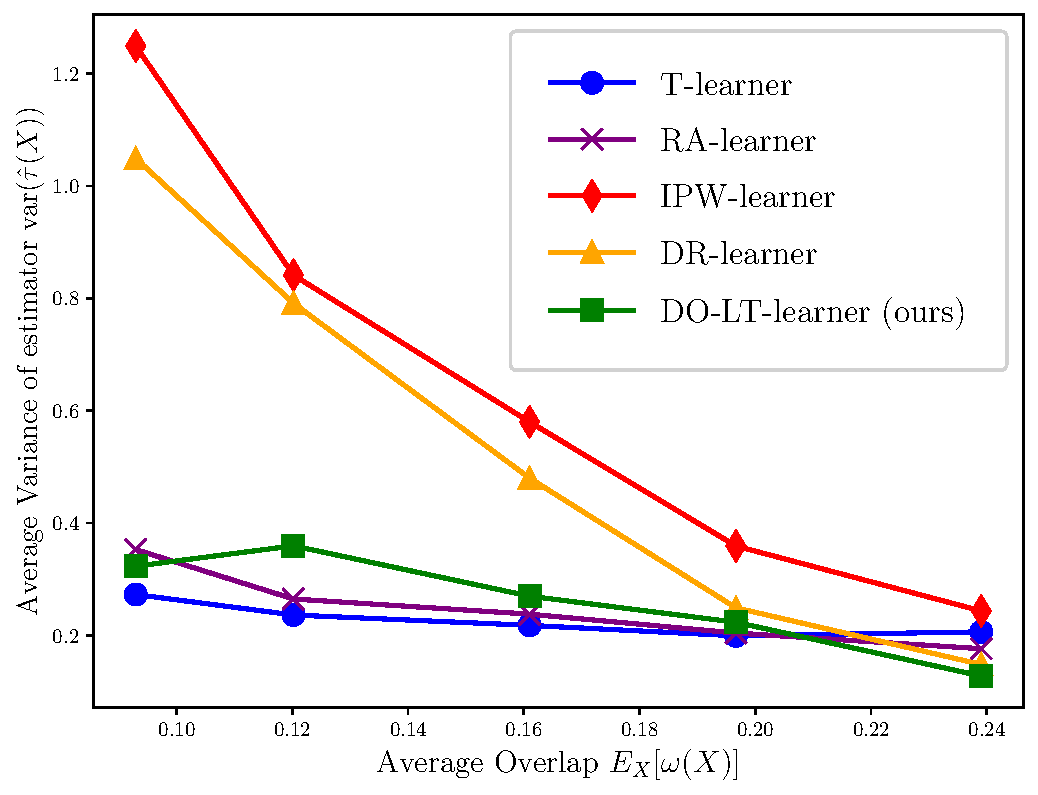
\includegraphics[width=\linewidth]{images/variance_vs_overlap.pdf}
  \caption{\textbf{Variance of estimator across different overlap scenarios ($\gamma$):}
  Low overlap leads to a high finite-sample variance of the DR-learner, while our \methods are robust and maintain a low variance.}
  \label{fig:estimator-variance-overlap}
  \vspace{-0.4cm}
\end{wrapfigure}

%\textbf{$\bullet$\,Overall performance underf overlap:} We simulate synthetic data to mimic four types of overlap scenarios: a) no overlap issue, b) treatment overlap, c) observation overlap, and d) mixed overlap. Under each scenarios, we evaluate the performance of three instantiations of our \method. 
%\underline{\textit{Results:}} Table~\ref{tab:synthetic-main} shows that our meta-learners outperform the baselines in the precision in estimation of heterogeneous effects (PEHE) in synthetic data. The unweighted DR-learner achieves lowest PEHE in the ideal "No overlap" setting, while suffers from high variance when overlap issue exists. The simplest T-learner, achieves fair performance as it does not leverage inverse propensities. In constrast, our learners achieve the lowest PEHE in respective overlap scenarios. For instance, the TO-learner outperforms in "Treatment overlap" scenario. And in the "mixed" scenario, the full \methods outperforms both the baseline learners and the single-overlap instantiations(TO/OO) with a relative improvement of $50.3\%$. Furthermore, lower PEHE std. of the weighted learners confirm that overlap-based retargeting effectively stabilizes finite-sample variance.

\textbf{$\bullet$\,Ablations w.r.t. orthogonality: } In this experiment, we analyze why Neyman-orthogonality is crucial for robustness. Here, we vary the sample sizes, where a lower sample size implies that the nuisance function estimation is more difficult. In addition to the existing baselines, we add two ablations: weighted but non-orthogonal versions of the LT-RA-learner and LT-O-DR-learner (see Appendix~\ref{app:baselines} for details). These ablations also employ overlap-based retargeting, allowing us thus to isolate the effect of Neyman-orthogonality. \underline{\textit{Results:}} The left panel of Figure~\ref{fig:neyman} shows that the orthogonal \DO consistently outperforms non-orthogonal ablations in finite-sample regimes. The right panel further illustrates how nuisance function estimation performance deteriorates as the sample size decreases. Taken together, these results show that our orthogonal \methods remain robust, thus effectively mitigating the bias induced by nuisance estimation errors.




\begin{figure}
    \centering
    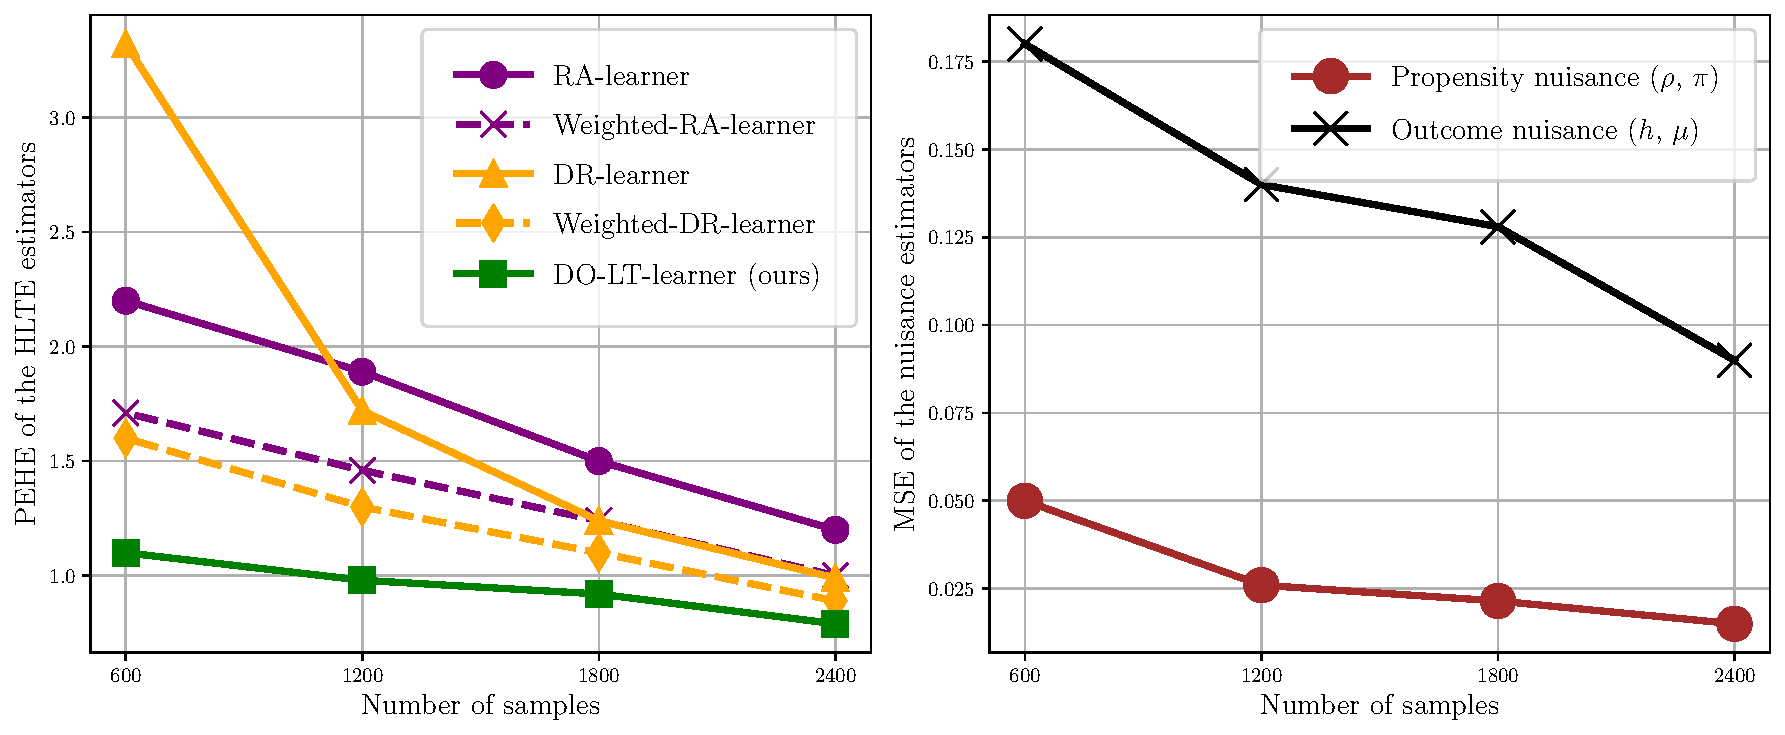
\includegraphics[width=1.0\linewidth]{images/sample_size_effects.pdf}
    \caption{\textbf{Benefit of Neyman-orthogonality:} (\textit{Left})~PEHE vs. sample size. The orthogonal LT-O-DO-learner outperforms the weighted (but non-orthogonal) DR/RA-learner. (\textit{Right})~Mean squared error (MSE) of the nuisance estimation. Taken together, high errors in the nuisance functions at small sample sizes drive the instability of non-orthogonal baselines.}
    \label{fig:neyman}
    \vspace{-0.5cm}
\end{figure}

\textbf{Experiments with medical data:} We evaluate the performance of the meta-learners under different types of overlaps in a medical context. Specifically, we consider a surrogate variable (7-day outcome) and a long-term outcome (6-month recovery status) based on the real-world patient covariates from the Third International Stroke Trial (IST-3)~\cite{Sandercock.2008-IST}. We again create 4 scenarios: $\mathcal{D}_*, \mathcal{D}_t, \mathcal{D}_o, \mathcal{D}_{t+o}$, which correspond to no overlap issue, low treatment overlap only, low long-term outcome overlap only, and mixed overlap issue (see Appendix~\ref{app:semi-synthetic} for details).  \underline{\textit{Results:}} Table~\ref{tab:semi-syn-main} shows the mean and standard deviation of PEHE on the semi-synthetic dataset. While all models perform similarly under ideal overlap ($\mathcal{D}_*$: no overlap issue), our proposed learners are superior in low-overlap regimes. Notably, in the scenario with both overlap issues ($\mathcal{D}_{t+o}$), our \DO reduces the estimation error by $40.6\%$ compared to the best baseline (\LTRA). This again demonstrates that our proposed learners are highly effective in the presence of overlap issues.

% Semi-synthetic data allows us to test the model under more realistic setting while providing the ground-truth to the true HLTE.

\textbf{Conclusion:} We develop a novel class of orthogonal meta-learners for estimating HLTEs. Through empirical experiments, we demonstrate that our method achieves superior robustness in low-overlap regimes.

\section*{Impact statement}
This work is purely methodological and aims to improve the stability of heterogeneous long-term treatment effect estimation under limited overlap. We do not foresee direct negative societal impact of this work.












\bibliography{example_paper}
\bibliographystyle{icml2026}


%%%%%%%%%%%%%%%%%%%%%%%%%%%%%%%%%%%%%%%%%%%%%%%%%%%%%%%%%%%%%%%%%%%%%%%%%%%%%%%
%%%%%%%%%%%%%%%%%%%%%%%%%%%%%%%%%%%%%%%%%%%%%%%%%%%%%%%%%%%%%%%%%%%%%%%%%%%%%%%
% APPENDIX
%%%%%%%%%%%%%%%%%%%%%%%%%%%%%%%%%%%%%%%%%%%%%%%%%%%%%%%%%%%%%%%%%%%%%%%%%%%%%%%
%%%%%%%%%%%%%%%%%%%%%%%%%%%%%%%%%%%%%%%%%%%%%%%%%%%%%%%%%%%%%%%%%%%%%%%%%%%%%%%
\newpage
\appendix
\onecolumn

%\section{Extension of related work}


\section{Theory}
\label{app:theory}

\subsection{Identification}
\label{app:identification}
In this section, we briefly demonstrate the identifiability of the heterogeneous long-term treatment effects under the surrogacy model. The identification of average long-term treatment effects is first shown by~\cite{Athey.2025}. We make a trivial extension to the heterogeneous setting. 
\begin{lemma}[Identification of HLTE]
    Under Assumptions~\ref{assumption-consistency} (Consistency), \ref{assumption-positivity} (Positivity), \ref{assumption-unconf} (Experimental Unconfoundedness), \ref{assumption-surrogacy} (Surrogacy), and \ref{assumption-compara} (Comparability), the heterogeneous long-term treatment effect $\tau^0(x)$ is identified as:
    \begin{align}
        \tau^0(x) = \mu(1,x) - \mu(0,x),
    \end{align}
    where $\mu(a,x) = \mathbb{E}[h(S,X) \mid A=a, X=x, R=0]$ and $h(s,x) = \mathbb{E}[Y \mid S=s, X=x, R=1]$.
\end{lemma}
\begin{proof}
    We begin with the definition of the causal estimand of interest:
    \begin{align}
        \tau^0(x) = \mathbb{E}[Y^1 - Y^0 \mid X=x, R=0].
    \end{align}
    To estimate $\tau^0$, it suffices to identify the conditional expectation of the potential outcome $\mathbb{E}[Y^a \mid X=x, R=0]$ for any $a \in \{0,1\}$.
    
    First, using Assumption~\ref{assumption-consistency} (Consistency) and Assumption~\ref{assumption-unconf} (Unconfoundedness), we can relate the potential outcome to the conditional expectation given the treatment assignment $A=a$:
    \begin{align}
        \mathbb{E}[Y^a \mid X=x, R=0] &= \mathbb{E}[Y^a \mid A=a, X=x, R=0] \nonumber \\
        &= \mathbb{E}[Y \mid A=a, X=x, R=0].
    \end{align}
    Then, we apply the tower law for expectation by conditioning on the surrogate variable $S$:
    \begin{align}
    \label{eq:proof-ident}
        \mathbb{E}[Y \mid A=a, X=x, R=0] &= \mathbb{E}_{S} \Big[ \mathbb{E}[Y \mid S, A=a, X=x, R=0] \Big| A=a, X=x, R=0 \Big].
    \end{align}
    We invoke Assumption~\ref{assumption-surrogacy} (Surrogacy), which states that $A \indep Y \mid S, X, R=0$. This allows us to remove the conditioning on $A$ in the inner expectation:
    \begin{align}
        \mathbb{E}[Y \mid S, A=a, X=x, R=0] = \mathbb{E}[Y \mid S, X, R=0].
    \end{align}
    Since the long-term outcome $Y$ is not observed in the experimental dataset $\mathcal{D}_1$ ($R=0$), we require Assumption~\ref{assumption-compara} (Long-term outcome comparability), specifically $Y \indep R \mid S, X$, to transport the outcome model from the observational dataset $\mathcal{D}_2$:
    \begin{align}
        \mathbb{E}[Y \mid S, X, R=0] &= \mathbb{E}[Y \mid S, X, R=1] \nonumber \\
        &= h(S,X).
    \end{align}
    Substituting this back into Eq.~(\ref{eq:proof-ident}), we get:
    \begin{align}
        \mathbb{E}[Y^a \mid X=x, R=0] &= \mathbb{E}_{S} \Big[ h(S,X) \Big| A=a, X=x, R=0 \Big] \nonumber \\
        &= \mu(a,x).
    \end{align}
   Hence:
    \begin{align}
        \tau^0(x) = \mu(1,x) - \mu(0,x).
    \end{align}
\end{proof}


\subsection{Efficient influence function}
\label{app:eif}

\paragraph{What is the efficient influence function (EIF)? } The EIF is a fundamental concept in semiparametric statistics that describes the sensitivity of an estimator to the underlying data distribution. Formally, consider a functional $\psi(\mathbb{P})$ of the data distribution $\mathbb{P}$ ((in our case $\psi(\mathbb{P})=\mathbb{E}_{S}[\mathbb{E}[Y \mid S, X, R=1]| A=1, X=x, R=0]- \mathbb{E}_{S}[\mathbb{E}[Y \mid S, X, R=1]| A=0, X=x, R=0]$)). The influence function $\phi(Z)$ of an estimator $\hat{\psi}$  is defined as the Gateaux derivative of the functional at $\mathbb{P}$ in the direction of a point mass $\delta_Z$~\cite{Hampel.1974}:
\begin{align}
    \lim_{\epsilon \to 0} \frac{\psi((1-\epsilon)\mathbb{P} + \epsilon \delta_Z) - \psi(\mathbb{P})}{\epsilon} = \phi(Z).
\end{align}

To illustrate this in our context, consider the Average Long-Term Treatment Effect (ALTE), $\tau = \mathbb{E}[\tau^0(X)]$. The EIF for the ALTE in the standard surrogacy model is given by the centered version of the doubly-robust pseudo-outcome derived in Eq.~(\ref{DR-pseudo-outcome}):
\begin{align}
    \phi_{ALTE}(Z) = \mathcal{T}_\mathrm{DR}(Z;\eta) - \tau.
\end{align}
First derived by \citet{Chen.2023, Athey.2025}, this EIF defines the \textbf{efficiency bound} of the ALTE estimation. An estimator is asymptotically efficient (i.e., it achieves the lowest possible asymptotic variance, known as the Cram\'er-Rao lower bound) if and only if it is asymptotically linear with influence function equal to the EIF~\cite{Bickel.1993, Tsiatis.2006}.

\paragraph{Properties of EIF}
The EIF has two properties that are critical for constructing robust two-stage learners:
\begin{enumerate}
    \item \textbf{Mean Zero:} The expectation of the influence function is zero, i.e., $\mathbb{E}[\phi(Z)] = 0$. This implies that the uncentered EIF (or pseudo-outcome), i.e. $\mathcal{T}_\mathrm{DR}(Z)$, is an unbiased estimator of the target parameter: $\mathbb{E}[\mathcal{T}_\mathrm{DR}(Z)] = \tau$.
    
    \item \textbf{Neyman-orthogonality:} The most important property is that the EIF is insensitive to perturbations in the nuisance parameters $\eta$. Mathematically, the G\^ateaux derivative of the expected EIF with respect to the nuisance functions is zero:
    \begin{align}
        \frac{\partial}{\partial r} \mathbb{E}\left[ \phi(Z; \eta + r(\hat{\eta} - \eta)) \right] \bigg|_{r=0} = 0.
    \end{align}
    This \emph{orthogonality} condition implies that the estimation error of the nuisance functions $\hat{\eta} - \eta$ affects the final target estimate $\tau$ only at a second-order rate (i.e., $\|\hat{\eta} - \eta\|^2$). This allows the final estimator to be still $\sqrt{n}$-consistent even if the nuisance components are estimated at slower rates (e.g., $n^{-1/4}$), which is common when using machine learning methods~\cite{Chernozhukov.2018}.
\end{enumerate}


\paragraph{Connection between EIF and DR-pseudo-outcome}
In our setting, we estimate a \textbf{conditional parameter} $\tau^0(x)$ instead of a scalar parameter $\tau^0$. The connection between the EIF and the \emph{EIF-based pseudo-outcome} (or equivalently, DR-pseudo-outcome) used in DR-learner~\cite{Kennedy.2020-DR-learner} is that the EIF-based pseudo-outcome is constructed to be the \textit{uncentered} EIF of the corresponding average effect, conditioned on covariates $X$.

Specifically, let $\mathcal{T}_\mathrm{DR}(Z)$ be the uncentered EIF for the average long-term effect, we use it to approximate the unobserved individual treatment effect $Y(1)-Y(0)$ because:
\begin{align}
    &\mathbb{E}[\mathcal{T}_\mathrm{DR}(Z) \mid X=x, R=0] = \tau^0(x) \\
    &\mathbb{E}[\mathcal{T}_\mathrm{DR}(Z) \mid X=x, R=1] = 0.    
\end{align}
By defining a loss function $\mathcal{L}(g) = \mathbb{E}[\1(R=0)g(X)^2 - 2\mathcal{T}_\mathrm{DR}g(X)]$, the minimizer is the conditional expectation $\mathbb{E}[\mathcal{T}_\mathrm{DR}|X, R=0]$, which recovers $\tau^0(x)$. Crucially, because $\mathcal{T}_\mathrm{DR}(Z)$ inherits the orthogonality property of the EIF, the second stage regression retains robustness against nuisance estimation errors. 

\paragraph{Semantics of Neyman-orthogonality: Functional vs. Loss} In this paper we frequently use the concept of Neyman-orthogonality. We point out that actually they differ in their target object and semantic implication:

\begin{itemize}
    \item \textbf{Functional Orthogonality:} 
    Primarily used for scalar parameters $\theta$ (e.g., ATE) defined by a moment condition $\mathbb{E}[\psi(Z; \theta, \eta)] = 0$. Orthogonality requires $\partial_\eta \mathbb{E}[\psi(Z; \theta_0, \eta_0)] = 0$~\cite{Chernozhukov.2018}. It ensures that nuisance estimation error $\hat{\eta} - \eta$ only has second-order impact on the target parameter $\hat\theta$.

    \item \textbf{Loss Orthogonality:} 
    Used for learning target functions $g(\cdot)$ (e.g., CATE/HLTE) via risk minimization $\min_g \mathcal{L}(g, \eta)$. Orthogonality requires the \textbf{cross-derivative} to vanish: $D_\eta D_g \mathcal{L}(g_0, \eta_0) = 0$~\cite{Foster.2023}.It ensures that distortions in $\hat{\eta}$ may change the shape of the loss landscape but do not shift the \emph{location} of the minimizer $g^*$ to the first order.

\end{itemize}


\subsection{EIF of the $\omega$-weighted average long-term effects}
\label{app:EIF-weighted-ATE}
The efficient influence function for the parameter $\tau^0_\omega$ in Eq.~(\ref{eq:walte-def}) is given by:
\begin{align}
\label{eq:eif-explicit}
\phi(Z; \eta) = \frac{1}{p_0 D_\omega} \Bigg[ &\1(R=0) \omega(X) \big( \hat{\tau}_{AIPW}(Z;\eta) - \tau^0_\omega \big) 
+ \1(R=1) \omega(X) \psi_{obs}(Z;\eta) + \big( \tau^0(X) - \tau^0_\omega \big) \Omega(Z;\eta) \Bigg],
\end{align}
where $p_0 = P(R=0)$ and $D_\omega = \mathbb{E}[\omega(X)|R=0]$. For simplicity, we use the shorthand $\omega(X) \equiv \omega(\pi(X), \rho(X))$. The components are defined as:
\begin{align}
    \hat{\tau}_{AIPW}(Z;\eta) &= \mu(1,X) - \mu(0,X) \notag  + \frac{A}{\pi(X)}(h(S,X) - \mu(1,X)) - \frac{1-A}{1-\pi(X)}(h(S,X) - \mu(0,X)) \\
    \psi_{obs}(Z;\eta) &= \frac{1-\rho_s(S,X)}{\rho_s(S,X)} \left( \frac{\pi_s(S,X) - \pi(X)}{\pi(X)(1-\pi(X))} \right) \big( Y - h(S,X) \big) \\
    \Omega(Z;\eta) &= \1(R=0) \frac{\partial \omega}{\partial \pi} (A - \pi(X)) + (1-\rho(X)) \frac{\partial \omega}{\partial \rho} (R - \rho(X)).
\end{align}

\begin{lemma}[Neyman-orthogonality]
\label{lemma:orthogonality}
    $\phi(Z; \eta)$ is the efficient influence function, which satisfies the Neyman-orthogonality condition with respect to the complete set of nuisance functions $\eta = (\pi(x), \pi_s(S,X), \rho(x), \rho_s(S,X), h(s,x), \mu(a,x))$. That is, the G\^ateaux derivative of the expected EIF vanishes at the true nuisance parameters:
    \begin{align}
        \partial_r \mathbb{E}\left[ \phi(Z; \eta + r\delta) \right] \big|_{r=0} = 0,
    \end{align}
    for any valid direction $\delta = \hat{\eta} - \eta$.
\end{lemma}
We provide a proof in Appendix~\ref{app:proof-neyman}.

%\section{Extension to observational population}
%\label{app:extension}

\subsection{On the optimality of the weighted efficiency bound}






\section{Instantiations}

\subsection{Derivation of the \TO}
\label{app:TO-LT-learner}
To derive the \TO, we set the weighting function to $\omega(X) = \pi(X)(1-\pi(X))$ to specifically target treatment overlap. We substitute this into the LT-weighting function $\omega^*(Z;\eta)$ in Eq.~(\ref{omega-star-def}) and LT-pseudo-outcome $\mathcal{T}_\mathrm{LT}(Z;\eta)$ in Eq.~(\ref{Tau-LT-def}). 

First, the residual term $\Omega(Z;\eta)$ simplifies to:
\begin{align}
    \Omega(Z;\eta) &= \1(R=0)\frac{\partial \omega}{\partial \pi}(A-\pi(X)) = \1(R=0)(1-2\pi(X))(A-\pi(X)).
\end{align}
%
Then, we substitute this back into $\omega^*$:
\begin{align}
\omega^*(Z;\eta) &= \1(R=0)\big[\pi(X)(1-\pi(X)) + (1-2\pi(X))(A-\pi(X))\big] = \1(R=0)(A-\pi(X))^2.
\end{align}
%
Next, we derive the LT-pseudo-outcome $\mathcal{T}_\mathrm{LT}$:
\begin{align}
\mathcal{T}_\mathrm{LT} &= \1(R=0)\Big[ \pi(1-\pi)\hat{\tau}_\mathrm{AIPW} + (\mu_1-\mu_0)(1-2\pi)(A-\pi) \Big] + \1(R=1)\pi(1-\pi)\psi_\mathrm{obs} \notag \\
&= \1(R=0)\Big[ (\mu_1-\mu_0)(A-\pi)^2 + (A-\pi)(h(S,X)-\mu(A, X)) \Big] + \1(R=1)\frac{1-\rho_s}{\rho_s}\big(\pi_s-\pi\big)\big(Y-h\big) \notag \\
&=\1(R=0) (A-\pi)\Big[ (\mu_1-\mu_0)(A-\pi) + h(S,X)- A\mu_1-(1-A)\mu_0 \Big] + \1(R=1)\frac{1-\rho_s}{\rho_s}\big(\pi_s-\pi\big)\big(Y-h\big)\notag \\
&= \1(R=0) (A-\pi)\Big[ h(S,X)- \underbrace{(\pi\mu_1 + (1-\pi)\mu_0)}_{=\E[h(S,X)\mid X,R=0]:=m(X)} \Big] + \1(R=1)\underbrace{\frac{1-\rho_s}{\rho_s}\big(\pi_s-\pi\big)\big(Y-h\big)}_{:=\psi_t}.
\end{align}
%
Plugging $\omega^*$ and $\mathcal{T}_\mathrm{LT}$ into the loss $\mathcal{L}_\omega = \mathbb{E}_n [\omega^* g^2 - 2\mathcal{T}_\mathrm{LT} g]$ and completing the square for the $R=0$ component yields the final \TO loss function:
\begin{align}
& \mathcal{L}_{\pi(1-\pi)}(g;\eta)=\mathbb{E}\Bigl[ \1(R=0)\bigl((h(S,X)-m(X))-(A -\pi(X))g(X)\bigr)^2 - 2\1(R=1)\psi_{t}(Z;\eta),g(X)\Bigr].
\end{align}
This example best demonstrates the advantage of weighting: After reweighting, the inverse propensities of treatment $A$ get eliminated. Therefore, the \TO avoids division by treatment propensities, which makes the learner more robust against low treatment overlap. 

\textbf{Remark:} The \TO is very similar to the standard R-learner~\citep{Nie.2021}, whose second-stage loss is defined via $(Y-m(X) - (A-\pi(X))g(X))^2$. We point out that the $\1(R=0)$ component of our \TO merely replaces $Y$ with the surrogate index $h$. To account for the first-order error of $h$, the $\1(R=1)$ is added to correct this nuisance estimation error, ensuring the orthogonality of the loss.

\subsection{Other possible instantiations}
In the main text, we provide three instantiations, which are the \TO, the \LO and the \DO. In fact, there are more instantiations that are also found to be helpful:

\textbf{LT-O-LO$\frac{1}{2}$-learner:} We consider an alternative weighting function $\omega(x)=\sqrt{\rho(x)}$ to provide a smaller penalty for low long-term outcome overlap. The corresponding LT-weighting function and LT-pseudo-outcome are given by:



\begin{align*}
    &\omega^*(Z;\eta) = \begin{cases} 
       \frac{\sqrt{\rho(X)}(1+\rho(X))}{2}, & \text{if } R=0, \\
       \frac{(1-\rho(X))^2}{2\sqrt{\rho(X)}}, & \text{if } R=1.
    \end{cases} \\
    &\mathcal{T}_\mathrm{LT}(Z;\eta) = \mu(1,X)-\mu(0,X) \notag \\
    &\quad + \begin{cases} 
      \frac{2}{1+\rho(X)}\left(\frac{A-\pi}{\pi(1-\pi)}(h(S,X)-\mu(A,X) \right), & \text{if } R=0, \\
      \frac{2\rho(X)}{(1-\rho(X))^2} \psi_\mathrm{obs}(Z;\eta), & \text{if } R=1.
    \end{cases}
\end{align*}




\newpage
\section{Proofs}
\label{app:proofs}
In the following section, we make use of the following properties:

\textbf{(1) $\E\left[\Omega(Z;\eta) \mid X\right]=0$}: 
\begin{align}
\label{eq:Omega-mean-zero-property}
    \E\left[\Omega(Z;\eta) \mid X\right] &= \E\left[\1(R=0) \frac{\partial \omega}{\partial \pi} (A - \pi(X)) + (1-\rho(X)) \frac{\partial \omega}{\partial \rho} (R - \rho(X)) \mid X\right] \notag \\
    &=(1 - \rho(X))\E\left[\frac{\partial \omega}{\partial \pi} (A - \pi(X))\mid X, R = 0\right] \notag \\
    &= 0. \qquad \qquad \qquad \qquad  \qquad \qquad(\text{By definition, } \pi(X)=\E\left[A\mid X,R=0\right])
\end{align}

\textbf{(2) $\E\left[\omega^*(Z;\eta) \mid X\right]=(1-\rho(X))\omega(X)$}: 

Since $\E\left[\Omega(Z;\eta) \mid X\right]=0$ and
\begin{align}
    \omega^*(Z;\eta) &= \1(R=0) \omega(X) + \Omega(Z;\eta),
\end{align}
we have 
\begin{align}
    \E\left[\omega^*(Z;\eta) \mid X\right]= \E\left[\1(R=0) \omega(X)\right] = (1-\rho(X))\omega(X)
\end{align}

\textbf{(3)  $\E\left[\1(R=1)\psi_{obs}(Z;\eta) \mid X\right] = 0$}:
\begin{align}
\label{eq:psi-mean-zero-property}
    \E\left[\1(R=1)\psi_{obs}(Z;\eta) \mid X\right] &= \rho(X) \E\left[\frac{1-\rho_s(S,X)}{\rho_s(S,X)} \left( \frac{\pi_s(S,X) - \pi(X)}{\pi(X)(1-\pi(X))} \right) \big( Y - h(S,X) \mid X, R=1\right] \notag \\
    &= \rho(X) \E_S\left[ \frac{1-\rho_s(S,X)}{\rho_s(S,X)} \left( \frac{\pi_s(S,X) - \pi(X)}{\pi(X)(1-\pi(X))} \right)\E_Y\left[ \big( Y - h(S,X) \mid S, X, R=1\right] \mid X, R=1\right]=0.
\end{align}

\textbf{(4) $\E\left[\hat{\tau}_{AIPW}(Z;\eta)\mid X, R=0\right]=\tau^0(X)$}:
\begin{align}
\E\!\left[\hat{\tau}_{AIPW}(Z;\eta)\mid X, R=0\right]
&=\E\!\left[
\mu(1,X)-\mu(0,X)
+\frac{A}{\pi(X)}\big(h(S,X)-\mu(1,X)\big)
-\frac{1-A}{1-\pi(X)}\big(h(S,X)-\mu(0,X)\big)
\ \Bigm|\ X,R=0\right] \notag\\
&=\mu(1,X)-\mu(0,X)
+\E\!\left[
\E\!\left[\frac{A}{\pi(X)}\big(h(S,X)-\mu(1,X)\big)\Bigm|X,A,R=0\right]
\Bigm|X,R=0\right] \notag\\
&\quad
-\E\!\left[
\E\!\left[\frac{1-A}{1-\pi(X)}\big(h(S,X)-\mu(0,X)\big)\Bigm|X,A,R=0\right]
\Bigm|X,R=0\right]. \notag
\end{align}
For the first augmentation term, using that $\pi(X)$ and $\mu(1,X)$ are $X$-measurable and that $A\in\{0,1\}$,
\begin{align}
\E\!\left[\frac{A}{\pi(X)}\big(h(S,X)-\mu(1,X)\big)\Bigm|X,A,R=0\right]
&=\frac{A}{\pi(X)}\Big(\E[h(S,X)\mid X,A,R=0]-\mu(1,X)\Big).\label{eq:aipw-term1-cond}
\end{align}
When $A=1$, by definition of $\mu(1,X)$,
\begin{align}
\E[h(S,X)\mid X,A=1,R=0]=\mu(1,X),
\end{align}
so the bracket in \eqref{eq:aipw-term1-cond} is zero; when $A=0$,  $A/\pi(X)=0$. Hence,
\begin{align}
\E\!\left[\frac{A}{\pi(X)}\big(h(S,X)-\mu(1,X)\big)\Bigm|X,R=0\right]=0.
\label{eq:aipw-term1-zero}
\end{align}
And with the same derivation, we have $\E\!\left[\frac{1-A}{1-\pi(X)}\big(h(S,X)-\mu(0,X)\big)\Bigm|X,A,R=0\right]=0$.
Therefore, 
\begin{align}
\label{eq:tau-AIPW-mean-tau}
\E\!\left[\hat{\tau}_{AIPW}(Z;\eta)\mid X, R=0\right]
=\mu(1,X)-\mu(0,X)=\tau^0(X).
\end{align}

\textbf{(5) $\E\left[\mathcal{T}_\mathrm{LT}(Z;\eta) \mid X\right] = (1-\rho(X))\omega(X) \tau^0(X)$:}

By definition, 
\begin{align}
    \mathcal{T}_\mathrm{LT}(Z;\eta) =  \1(R=0) \omega(X) \hat{\tau}_\mathrm{AIPW}(Z;\eta)
     +  \1(R=1) \cdot\omega(X) \psi_\mathrm{obs}(Z;\eta) + (\mu(1,X)-\mu(0,X)) \Omega(Z;\eta),\notag
\end{align}
Using properties (1), (3) and (4) from above, we have immediately that $\E\left[\mathcal{T}_\mathrm{LT}(Z;\eta) \mid X\right] = (1-\rho(X))\omega(X) \tau^0(X).$

\subsection{Variance analysis}
\label{app:variance}
Here, we formally state the variance of the long-term DR-pseudo-outcome:

\begin{lemma}[Variance of DR-pseudo-outcome]
\label{lemma-variance}
The variance of DR-pseudo-outcome is
%\vspace{-0.3cm}

\begin{align*}
    \var(\mathcal{T}_\mathrm{DR} \mid X) \geq \underbrace{(1-\rho(X)) \cdot \Sigma_{t}(X)}_{\text{treatment overlap}} + \underbrace{\rho(X) \cdot \Sigma_{\text{o}}(X)}_{\text{long-term outcome overlap}}
\end{align*}

\vspace{-0.6cm}
\footnotesize
\begin{align*}
    \Sigma_{t}(X) &= \mathbb{E}\Bigl[ \left(\frac{1}{\pi(X)(1-\pi(X))}\right)^2 \sigma_h(A,X) \,\big|\, X \Bigr]  \\
    \Sigma_{\text{o}}(X) &= \mathbb{E}_{S|X} \left[ \left(\frac{1-\rho_s(S,X)}{\rho_s(S,X)}\left(\frac{\pi_s-\pi}{\pi(1-\pi)}\right)\right)^2 \sigma_y(S,X) \right],
\end{align*}
where $\sigma_h(X,A)=\var(h(S,X)|X,A,R=0)$, $\sigma_y(S,X)=\var(Y|S,X,R=1)$.
\normalsize
\end{lemma}

This is similar to the variance analysis from \citet{Fisher.2023}. When the treatment overlap $\pi(x)(1-\pi(x)$ is close to zero, both $\Sigma_t(x)$ and $\Sigma_o(x)$ become very large. When there is limited long-term outcome overlap, namely $\rho(x)$ close to zero (and thus for $\rho_s(S,X)$ as well),  we have that $\rho(x)\Sigma_o(x)$ scales roughly with $\E[\frac{1}{\rho_s(S,X)}|X=x]$. Therefore, $\mathcal{T}_\mathrm{DR}$ has a high variance when at least one of the overlaps is low. As a result, the \DR is \emph{not} robust against low overlap.


\textbf{Proof.}
By the Law of Total Variance, conditioning on the dataset indicator $R$, we have:
\begin{align}
    \var(\mathcal{T}_{\mathrm{DR}} \mid X) &= \mathbb{E}_R[\var(\mathcal{T}_{\mathrm{DR}} \mid X, R) \mid X] + \var_R(\mathbb{E}[\mathcal{T}_{\mathrm{DR}} \mid X, R] \mid X) \\
    &\geq \mathbb{E}_R[\var(\mathcal{T}_{\mathrm{DR}} \mid X, R) \mid X]
\end{align}
where the inequality holds because variance is non-negative. Expanding the expectation over $R \in \{0, 1\}$ with $\rho(X) = \mathbb{P}(R=1|X)$, we obtain:
\begin{equation}
    \var(\mathcal{T}_{\mathrm{DR}} \mid X) \geq (1-\rho(X)) \underbrace{\var(\mathcal{T}_{\mathrm{DR}} \mid X, R=0)}_{\text{(A)}} + \rho(X) \underbrace{\var(\mathcal{T}_{\mathrm{DR}} \mid X, R=1)}_{\text{(B)}} \label{eq:total_var}
\end{equation}

\textbf{Part (A): Treatment Overlap Instability ($R=0$).}
In the experimental dataset ($R=0$), $\mathcal{T}_{\mathrm{DR}}$ reduces to the AIPW estimator:
\begin{align}
    \hat\tau_{\mathrm{AIPW}}=\frac{A-\pi(X)}{\pi(X)(1-\pi(X))}(h(S,X) - \mu(A,X)) + \mu(1,X)-\mu(0,X):=Z_0 + \mu(1,X)-\mu(0,X).
\end{align}
Hence, we have
\begin{align}
    \var(\mathcal{T}_{\mathrm{DR}} \mid X, R=0)) &= \var(\hat\tau_{\mathrm{AIPW}} \mid X, R=0)) \notag \\
    &= \var\left(\frac{A-\pi(X)}{\pi(X)(1-\pi(X))}(h(S,X) - \mu(A,X))\mid X, R=0\right) \notag \\
    &= \mathbb{E}_{A}[\text{Var}(Z_0 \mid A, X)] + \text{Var}_{A}(\underbrace{\mathbb{E}[Z_0 \mid A, X]}_{=0})
\end{align}
The inner expectation is zero because $\mu(A,X) = \mathbb{E}[h(S,X)|A,X]$. Thus, we are left with the expected variance:
\begin{equation}
\label{Sigma_t}
    \Sigma_t(X) := \var(\mathcal{T}_{\mathrm{DR}} \mid X, R=0))=\var(Z_0 \mid X) = \mathbb{E}_{A|X} \left[ \left( \frac{A-\pi(X)}{\pi(X)(1-\pi(X))} \right)^2 \var(h(S,X) \mid A, X) \right]
\end{equation}

This term scales with $\frac{1}{\pi(X)^2(1-\pi(X))^2}$, causing high variance under limited treatment overlap.

\textbf{Part (B): Long-term outcome Overlap Instability ($R=1$).}
In the observational dataset ($R=1$), $\mathcal{T}_{\mathrm{DR}}$ uses the observation proxy $\psi_{\mathrm{obs}}$. Let:
$$
Z_1 = \frac{1-\rho_s(S,X)}{\rho_s(S,X)} W_{\pi}(S,X) (Y - h(S,X)),
$$
where $W_{\pi}(S,X)=\left( \frac{\pi_s(S,X) - \pi(X)}{\pi(X)(1-\pi(X))} \right)$.
Conditioning on the surrogate $S$, we get:
\begin{align}
    \var(Z_1 \mid X, R=1) = \mathbb{E}_{S}[\var(Z_1 \mid S, X, R=1)] + \var_{S}(\underbrace{\mathbb{E}[Z_1 \mid S, X, R=1]}_{=0}).
\end{align}
The inner expectation is zero because $h(S,X) = \mathbb{E}[Y|S,X, R=1]$. Thus:
\begin{align}
    \Sigma_o(X) := \var(Z_1 \mid X) = \mathbb{E}_{S|X} \left[ \left( \frac{1-\rho_s(S,X)}{\rho_s(S,X)} \right)^2 \left(\frac{\pi_s(S,X) - \pi(X)}{\pi(X)(1-\pi(X))} \right)^2 \var(Y \mid S, X) \right]
\end{align}
This term scales with $\frac{1}{\rho_s(S,X)^2}$, causing high variance under limited long-term outcome overlap.

Combining (A) and (B) together yields the lower bound:
\begin{align}
    \var(\mathcal{T}_{\mathrm{DR}} \mid X) \geq (1-\rho(X)) \Sigma_{t}(X) + \rho(X) \Sigma_{o}(X)
\end{align}


\subsection{Neyman-orthogonality}
\label{app:proof-neyman}
Let $\partial_g \mathcal{L}_\omega(g, \eta) = S(g, \eta) \cdot \dot{g}(X) $ be the derivative of the loss. By definition, the loss in Eq.~(\ref{eq:weighted-ortho-loss-tau0}) is orthogonal if we can show Neyman-orthogonality of the following term:
\begin{align}
    \partial_r \mathbb{E}[S(g, \eta + r\delta)] \big|_{r=0} = 0, \quad \forall \delta=\hat\eta-\eta.
\end{align}
The reason is that $\dot{g}(X)$ is irrelevant w.r.t. the nuisance $\eta$. The term can be written as:
\begin{align}
    \label{gradient-S}
    \E[S(g,\eta)] = \mathbb{E}\Big[ \1(R=0)\omega(X)(g(X) - \hat{\tau}_{AIPW}) - \1(R=1)\omega(X)\psi_{obs} - \big( (\mu(1,X)-\mu(0,X)) - g(X) \big) \Omega(Z;\eta)\Big].
\end{align}
where
\begin{align}
    \hat{\tau}_{AIPW}(Z;\eta) &= \mu(1,X) - \mu(0,X) \notag  + \frac{A}{\pi(X)}(h(S,X) - \mu(1,X)) - \frac{1-A}{1-\pi(X)}(h(S,X) - \mu(0,X)) \\
    \psi_{obs}(Z;\eta) &= \frac{1-\rho_s(S,X)}{\rho_s(S,X)} \left( \frac{\pi_s(S,X) - \pi(X)}{\pi(X)(1-\pi(X))} \right) \big( Y - h(S,X) \big) \\
    \Omega(Z;\eta) &= \1(R=0) \frac{\partial \omega}{\partial \pi} (A - \pi(X)) + (1-\rho(X)) \frac{\partial \omega}{\partial \rho} (R - \rho(X)).
\end{align}



\textbf{1. Orthogonality w.r.t. outcome nuisances $\mu(a,x)$:}

The nuisance $\mu(a,x)$ appears in $\hat{\tau}_{AIPW}$ and $(\mu(1,X)-\mu(0,X)) \Omega(Z;\eta)$. Let $\mu_r = \mu + r\delta_\mu$.
\begin{align}
    \partial_r \mathbb{E}[S]\Big|_{r=0} &= -\mathbb{E}\left[ \1(R=0)\omega(X) \partial_r \hat{\tau}_{AIPW} + (\delta_\mu(1) - \delta_\mu(0))\Omega(Z;\eta)\right] \notag \\
    &= -\mathbb{E}\left[ \1(R=0)\omega(X) \left( \delta_\mu(1) - \delta_\mu(0) - \frac{A}{\pi}(\delta_\mu(1)) + \frac{1-A}{1-\pi}(\delta_\mu(0)) \right) \right] \notag \\
    &= -\mathbb{E}_X\left[ \omega(X) (1-\rho(X))\E\left[ \delta_\mu(1) - \delta_\mu(0) - \frac{A}{\pi}(\delta_\mu(1)) + \frac{1-A}{1-\pi}(\delta_\mu(0)) \mid X, R=0 \right] \right]
\end{align}
Here we use the property that $\rho(x)=\E[R\mid X]$ (by definition), and $\E\left[\Omega \mid X\right]=0$ (see Eq.~(\ref{eq:Omega-mean-zero-property}). Conditioning on $X$ and $R=0$, and using $\mathbb{E}[A|X, R=0]=\pi(X)$:
\begin{align}
    \mathbb{E}[ \delta_\mu(1) - \delta_\mu(0) - \frac{A}{\pi}(\delta_\mu(1)) + \frac{1-A}{1-\pi}(\delta_\mu(0)) \mid X, R=0 ] = \delta_\mu(1)(1 - \frac{\pi}{\pi}) - \delta_\mu(0)(1 - \frac{1-\pi}{1-\pi}) = 0.
\end{align}
Therefore, we have that $\partial_r \mathbb{E}[S]\Big|_{r=0} = 0$.


\textbf{2. Orthogonality w.r.t. surrogate outcome $h(s,x)$:}

The nuisance $h$ appears in both $\hat{\tau}_{AIPW}$ and $\psi_{obs}$.
For the AIPW term, the derivative contribution is:
\begin{align}
    D_1 &= -\mathbb{E}\left[ \1(R=0)\omega(X) \left( \frac{A}{\pi}\delta_h - \frac{1-A}{1-\pi}\delta_h \right) \right] \notag \\
    &= -\E_X\left[(1-\rho(X))\mathbb{E}_S\left[ \omega(X) \frac{A - \pi}{\pi(1-\pi)} \delta_h \mid X, R=0\right]\right] \notag \\
    &= -\mathbb{E}_X\left[ (1-\rho(X))\E_{S}\left[\omega(X) \frac{\pi_s(S,X) - \pi}{\pi(1-\pi)} \delta_h \mid X, R=0\right]\right],
\end{align}
For the $\psi_{obs}$ term,  we make use of the density ratio property that $\frac{dP(S \mid R=1, X)}{dP(S \mid R=0, X)} = \frac{\rho_s(S,X)}{1-\rho_s(S,X)} \frac{P(R=0|X)}{P(R=1|X)}$ to transform the measure from the observational to the experimental sample:
\begin{align}
    D_2 &= -\mathbb{E}\left[ \1(R=1)\omega(X) \frac{1-\rho_s(S,X)}{\rho_s(S,X)} \frac{\pi_s(S,X)-\pi(X)}{\pi(1-\pi)} (-\delta_h) \right] \notag \\
    &= \mathbb{E}_{X}\left[\E_S\left[ \rho(X) \frac{1-\rho_s(S,X)}{\rho_s(S,X)} \omega(X) \frac{\pi_s(S,X) - \pi}{\pi(1-\pi)} \delta_h \mid X, R=1 \right]\right] \notag \\
    &=\mathbb{E}_{X}\left[\E_S\left[(1-\rho(X))\omega(X) \frac{\pi_s(S,X) - \pi}{\pi(1-\pi)} \delta_h \mid X, R=0\right]\right].
\end{align}
Thus $D_1 + D_2 = 0$.

\textbf{3. Orthogonality w.r.t. $\pi(x)$:}

Let $\pi_r(X)=\pi(X)+r\,\delta_\pi(X)$, then we take the derivative w.r.t. $r$:
\begin{align}
\partial_r \E[S(g,\eta+r\delta_\pi)]\Big|_{r=0}
&=
\E\Big[
\1(R=0)\,\partial_r\omega_r(X)\Big|_{r=0}\,\big(g(X)-\hat\tau_{AIPW,0}\big)
-\1(R=0)\omega(X)\,\partial_r\hat\tau_{AIPW,r}\Big|_{r=0} \Big] \notag \\
&\quad
-\E\Big[\1(R=1)\,\partial_r\omega_r(X)\Big|_{r=0}\,\psi_{obs,0}
+\1(R=1)\omega(X)\,\partial_r\psi_{obs,r}\Big|_{r=0}\Big] \notag \\
&\quad
-\E\Big[\big((\mu(1,X)-\mu(0,X))-g(X)\big)\,\partial_r\Omega_r(Z)\Big|_{r=0}\Big].
\label{eq:pi-derivative-decomp}
\end{align}

First, $\partial_r\omega_r(X)|_{r=0} = \frac{\partial\omega}{\partial\pi}(X)\,\delta_\pi(X)$. Then
\begin{align}
\label{F1}
    F_1:=\E\Big[
\1(R=0)\,\partial_r\omega_r(X)\Big|_{r=0}\,\big(g(X)-\hat\tau_{AIPW,0}\big)\Big] = \E\Big[\1(R=0)\frac{\partial\omega}{\partial\pi}(X)\,\delta_\pi(X) (g(X)-\tau^0(X))\Big]
\end{align}

Second, we have
\begin{align}
\label{proof-partial-pi-1}
    &\E\left[\1(R=0)\partial_r\hat\tau_{AIPW,r}\Big|_{r=0} \mid X\right] \\
    &= (1-\rho(X))\E\left[\partial_r\Bigl(\frac{A}{\pi_r(X)}\Bigr)\Big|_{r=0}(h(S,X) - \mu(1,X)) - \partial_r\Bigl(\frac{1-A}{1-\pi_r(X)}\Bigr)\Big|_{r=0}(h(S,X) - \mu(0,X)) \mid X, R=0\right] \notag \\
    &= (1-\rho(X))\E\left[A\frac{-1}{\pi(X)^2}\delta_\pi(X)(h(S,X) - \mu(1,X)) - (1-A)\frac{1}{(1-\pi(X))^2}\delta_\pi(X)(h(S,X) - \mu(0,X)) \mid X, R=0\right] \notag \\
    &= (1-\rho(X))\delta_\pi(X)\Biggl(\frac{-1}{\pi(X)^2} \underbrace{\E\left[A(h(S,X) - \mu(1,X))  \mid X, R=0\right]}_{=0} - \frac{1}{(1-\pi(X))^2}\underbrace{\E\left[(1-A)(h(S,X) - \mu(0,X)) \mid X, R=0\right]}_{=0}\Biggr) \notag \\
    &=0
\end{align}
The last equation is zero because $\forall a \in \{0,1\}, \quad \E\left[h(S,X) - \mu(a,X) \mid A=a, X,R=0\right]=0$. Hence
\begin{align}
    F_2:= \E\left[\omega(X)\1(R=0)\partial_r\hat\tau_{AIPW,r}\Big|_{r=0} \right] = 0.
\end{align}


From the property in Eq.~(\ref{eq:psi-mean-zero-property}), we have that $\E\left[\1(R=1)\psi_{obs}\mid X\right] = 0$. Furthermore, with the exact same derivation, we also have $\E\left[\1(R=1)\partial_r\psi_{obs,r} \mid X\right] = 0$ (because the $Y-h(S,X)$ is mean zero). Hence, the second row in Eq.~(\ref{eq:pi-derivative-decomp}) can be simplified to
\begin{align}
\label{proof-paritial-pi-2}
    F_3:=-&\E\Big[\1(R=1)\,\partial_r\omega_r(X)\Big|_{r=0}\,\psi_{obs,0}
+\1(R=1)\omega(X)\,\partial_r\psi_{obs,r}\Big|_{r=0}\Big] \notag \\
=& \E\Big[\partial_r\omega_r(X)\E\left[\1(R=1)\Big|_{r=0}\,\psi_{obs,0}\mid X\right]
+\omega(X)\,\E\left[\1(R=1)\partial_r\psi_{obs,r}\Big|_{r=0}\mid X\right]\Big] = 0.
\end{align}

Finally, we address the terms involving $\partial_r\Omega_r|_{r=0}$.
Since $\Omega_r=\1(R=0)\frac{\partial\omega}{\partial\pi_r}(A-\pi_r(X))+(1-\rho(X))\frac{\partial\omega}{\partial\rho}(R-\rho(X))$, we have
\begin{align}
\partial_r\Omega_r\Big|_{r=0}
&=\1(R=0)\left[
\frac{\partial^2\omega}{\partial\pi^2}(X)\,\delta_\pi(X)\,(A-\pi(X))
-\frac{\partial\omega}{\partial\pi}(X)\,\delta_\pi(X)
\right].
\label{eq:Omega-pi-derivative}
\end{align}
Conditioning on $X$ and $R=0$, and using $\E[A-\pi(X)\mid X,R=0]=0$,
\begin{align}
\E\!\left[\partial_r\Omega_r\Big|_{r=0}\ \Bigm|\ X\right]
&=
(1-\rho(X))\left[
\frac{\partial^2\omega}{\partial\pi^2}(X)\,\delta_\pi(X)\,\E[A-\pi\mid X,R=0]
-\frac{\partial\omega}{\partial\pi}(X)\,\delta_\pi(X)
\right] \notag\\
&=-(1-\rho(X))\frac{\partial\omega}{\partial\pi}(X)\,\delta_\pi(X).
\label{eq:Omega-pi-mean}
\end{align}
Therefore,
\begin{align}
\label{proof-NO-paritial-Omega}
F_4:=-\E\Big[\big((\mu(1,X)-\mu(0,X))-g(X)\big)\,\partial_r\Omega_r\Big|_{r=0}\Big]
&=
(1-\rho(X))\E\Big[\big(\tau^0(X)-g(X)\big)\frac{\partial\omega}{\partial\pi}(X)\delta_\pi(X)\Big].
\end{align}

Putting everything together, we have
\begin{align}
    \partial_r \E[S(g,\eta+r\delta_\pi)]\Big|_{r=0}=&F_1 + F_2+F_3+F_4 \notag \\
    =& \E\Big[\1(R=0)\frac{\partial\omega}{\partial\pi}(X)\,\delta_\pi(X) (g(X)-\tau^0(X))\Big] + \E\Big[(1-\rho(X))\frac{\partial\omega}{\partial\pi}(X)\,\delta_\pi(X)\big(\tau^0(X)-g(X)\big)\Big] \notag \\
    =&0.
\end{align}

\textbf{4. Orthogonality w.r.t. $\pi_s(s,x), \rho_s(S,X)$:}

Let $\pi_r(S,X)=\pi_s(S,X)+r\,\delta_{\pi_s}(S,X)$. Since $\pi_s(S,X)$ only appears in $\psi_{obs}$, therefore
\begin{align}
\partial_r\psi_{obs,r}\Big|_{r=0}
=\left(\partial_r (\frac{1-\rho_s(S,X)}{\rho_s(S,X)} \left( \frac{\pi_s(S,X) - \pi(X)}{\pi(X)(1-\pi(X))} \right))\Big|_{r=0}\right)\big(Y-h(S,X)\big).
\end{align}
Conditioning on $(S,X,R=1)$, we have $\E[Y-h(S,X)\mid S,X,R=1]=0$, and therefore by tower law
\begin{align}
\partial_r \E[S(g,\eta+r\delta_{\pi_s})]\Big|_{r=0} = -\E\left[\1(R=1)\omega(X)\,\partial_r\psi_{obs,r}\Big|_{r=0}\right]=0.
\end{align}
The same derivation applies for $\rho_s(S,X)$.

\textbf{5. Orthogonality w.r.t. $\rho(x)$:}

Let $\rho_r(X)=\rho(X)+r\,\delta_\rho(X)$. The nuisance $\rho(X)$ appears in $\omega(X)$ and in $\Omega(Z;\eta)$, but not in $\hat\tau_{AIPW}$ or $\psi_{obs}$.
Differentiating the gradient yields two types of terms:
\begin{align}
\partial_r \E[S(g,\eta+r\delta_\rho)]\Big|_{r=0}
&=
\E\Big[\partial_r\omega_r(X)\Big|_{r=0}\cdot\big(\1(R=0)(g-\hat\tau_{AIPW})-\1(R=1)\psi_{obs}\big)\Big] \notag\\
&\quad
-\E\Big[\big((\mu(1)-\mu(0))-g\big)\,\partial_r\Omega_r\Big|_{r=0}\Big].
\label{eq:rho-derivative-decomp}
\end{align}
For the first term, using properties in Eq.~(\ref{eq:tau-AIPW-mean-tau}) and Eq.~(\ref{eq:psi-mean-zero-property}), we have
\begin{align}
&\E\Big[\partial_r\omega_r(X)\Big|_{r=0}\cdot\big(\1(R=0)(g-\hat\tau_{AIPW})-\1(R=1)\psi_{obs}\big)\Big] \notag\\
&\qquad=
\E_X\Bigg[
\frac{\partial\omega}{\partial\rho}(X)\,\delta_\rho(X)\;
\E\Big[\1(R=0)\big(g(X)-\hat\tau_{AIPW}\big)-\1(R=1)\psi_{obs} \mid X\Big]
\Bigg] \notag\\
&\qquad=
\E_X\Bigg[
\frac{\partial\omega}{\partial\rho}(X)\,\delta_\rho(X)\;
\Big(
\Pr(R=0\mid X)\E[g(X)-\hat\tau_{AIPW}\mid X,R=0]
-\Pr(R=1\mid X)\E[\psi_{obs}\mid X,R=1]
\Big)
\Bigg] \notag\\
&\qquad=
\E_X\Bigg[
\frac{\partial\omega}{\partial\rho}(X)\,\delta_\rho(X)\;
(1-\rho(X))\big(g(X)-\tau^0(X)\big)
\Bigg].
\label{eq:rho-first-term}
\end{align}

For the second term, only the second component of $\Omega$ depends on $\rho(X)$:
\begin{align}
\Omega_r(Z)
=(1-\rho_r(X))\frac{\partial\omega}{\partial\rho_r}(X)\big(R-\rho_r(X)\big).
\end{align}
Thus 
\begin{align}
    \E\left[\partial_r\Omega_r|_{r=0} \mid X\right] = (1-\rho_r(X))\frac{\partial\omega}{\partial\rho_r}(X)\cdot -\delta_\rho
\end{align}
Since $(\mu(1,X)-\mu(0,X))-g(X)$ is $X$-measurable,
\begin{align}
-\E\Big[\big((\mu(1)-\mu(0))-g\big)\,\partial_r\Omega_r\Big|_{r=0}\Big]
&=
-\E_X\Big[
\big((\mu(1,X)-\mu(0,X))-g(X)\big)\,
\E\!\left[\partial_r\Omega_r\Big|_{r=0}\ \Bigm|\ X\right]
\Big] \notag\\
&=
\E_X\Big[
\big((\mu(1,X)-\mu(0,X))-g(X)\big)\,
(1-\rho(X))\frac{\partial\omega}{\partial\rho}(X)\,\delta_\rho(X)
\Big].
\label{eq:rho-second-term}
\end{align}
Adding the terms \eqref{eq:rho-first-term} and \eqref{eq:rho-second-term} together, we have
\begin{align}
\partial_r \E[S(g,\eta+r\delta_\rho)]\Big|_{r=0}
&=
\E_X\Big[
(1-\rho(X))\frac{\partial\omega}{\partial\rho}(X)\,\delta_\rho(X)
\Big\{\big(g(X)-\tau^0(X)\big)+\big(\mu(1,X)-\mu(0,X)-g(X)\big)\Big\}
\Big] \notag\\
&=
\E_X\Big[
(1-\rho(X))\frac{\partial\omega}{\partial\rho}(X)\,\delta_\rho(X)\cdot 0
\Big]=0.
\end{align}



Combining these results, the total derivative $\partial_r \mathcal{E}(\eta + r\delta)|_{r=0} = 0$, proving Neyman-orthogonality.


\subsection{Proof of Theorem~\ref{thm:equiv-loss}}
The loss $\mathcal{L}_\omega(g;\eta)$ is, up to a constant (w.r.t. $g$), equivalent with:
\begin{equation}
    \mathcal{R}_\omega(g;\eta)=\E\left[\1(R=0) \omega(X) \big(\hat{\tau}_{AIPW} -g \big)^2- 2\1(R=1) \omega(X) \psi_{obs}\cdot g + \Omega\big( (\mu(1,X)-\mu(0,X)) - g \big)^2\right].
\end{equation}
Recall that
\begin{equation}
    \psi_{obs}(Z;\eta) = \frac{1-\rho_s(S,X)}{\rho_s(S,X)} \left( \frac{\pi_s(S,X) - \pi(X)}{\pi(X)(1-\pi(X))} \right) \big( Y - h(S,X) \big).
\end{equation}
Hence, the conditional expectation of $\1(R=1)\psi_{obs}(Z;\eta)$ given $X$ equals zero:
\begin{align}
    \E\left[\1(R=1)\psi_{obs}(Z;\eta) \mid X\right] &= \E\left[ \1(R=1) \frac{1-\rho_s(S,X)}{\rho_s(S,X)} \left( \frac{\pi_s(S,X) - \pi(X)}{\pi(X)(1-\pi(X))} \right) \big( Y - h(S,X) \big) \Bigg| X \right] \\
    &= \E\left[ \1(R=1) \frac{1-\rho_s(S,X)}{\rho_s(S,X)} \left( \frac{\pi_s(S,X) - \pi(X)}{\pi(X)(1-\pi(X))} \right) \underbrace{\E[Y - h(S,X) \mid S, X, R=1]}_{=0} \Bigg| X \right] \\
    &= 0.
\end{align}
Note that the conditional expectation of $\Omega(Z;\eta)$ given $X$ is also zero:
\begin{align}
    \E\left[\Omega(Z;\eta) \mid X\right] &= \E\left[ \1(R=0) \frac{\partial \omega}{\partial \pi} (A - \pi(X)) + (1-\rho(X)) \frac{\partial \omega}{\partial \rho} (R - \rho(X)) \Bigg| X \right] \\
    &= \frac{\partial \omega}{\partial \pi} \E\left[\1(R=0)(A - \pi(X)) \mid X\right] + (1-\rho(X)) \frac{\partial \omega}{\partial \rho} \underbrace{\E\left[R - \rho(X) \mid X\right]}_{=0} \\
    &= \frac{\partial \omega}{\partial \pi} \Pr(R=0|X) \underbrace{\E\left[A - \pi(X) \mid X, R=0\right]}_{=0} = 0. \label{exp-Omega-zero}
\end{align}
Hence, the risk function simplifies to
\begin{equation}
\label{eq:simplified-risk}
    \mathcal{R}_\omega(g;\eta)=\E\left[\1(R=0) \omega(X) \big(\hat{\tau}_{AIPW}(Z;\eta) -g(X) \big)^2\right],
\end{equation}
where 
\begin{equation}
    \hat{\tau}_{AIPW}(Z;\eta) = \mu(1,X) - \mu(0,X) + \frac{A}{\pi(X)}(h(S,X) - \mu(1,X)) - \frac{1-A}{1-\pi(X)}(h(S,X) - \mu(0,X)).
\end{equation}
%
We further write the Eq.~(\ref{eq:simplified-risk}) as:
\begin{align}
    \mathcal{R}_\omega(g;\eta) &=\E\left[\1(R=0) \omega(X) \big(\hat{\tau}_{AIPW}(Z;\eta) -g(X) \big)^2\right] \\
    &= \E\left[\1(R=0) \omega(X) \big(\hat{\tau}_{AIPW}(Z;\eta)- \tau^0(X) + \tau^0(X) - g(X) \big)^2\right] \\
    &= \E\left[\1(R=0) \omega(X) \bigl(\hat{\tau}_{AIPW}(Z;\eta)- \tau^0(X)\bigr)^2\right] + \E\left[\1(R=0) \omega(X) \bigl(\tau^0(X) - g(X) \bigr)^2\right] \nonumber \\
    &\quad + 2\E\left[\1(R=0) \omega(X) \bigl(\hat{\tau}_{AIPW}(Z;\eta)- \tau^0(X)\bigr)\bigl(\tau^0(X) - g(X) \bigr)\right] \\
    &= \E\left[\1(R=0) \omega(X) \bigl(\hat{\tau}_{AIPW}(Z;\eta)- \tau^0(X)\bigr)^2\right] +  \E\left[\1(R=0) \omega(X) \bigl(\tau^0(X) - g(X)\bigr)^2\right] \\
    &= p_0 \E\left[\omega(X)\bigl(\tau^0(X) - g(X)\bigr)^2 \mid R=0\right] + \text{Const}_g \\
    &\propto p_0 \E\left[\omega(X)\bigl(\tau^0(X) - g(X)\bigr)^2 \mid R=0\right] = \mathcal{L}^{\text{oracle}}_\omega(g;\eta).
\end{align}
The reason the cross term in the decomposition is zero is because
\begin{align}
    &\E\left[\1(R=0) \omega(X) \bigl(\hat{\tau}_{AIPW}(Z;\eta)- \tau^0(X)\bigr)\bigl(\tau^0(X) - g(X) \bigr)\right] \nonumber \\
    &= \E\left[ \E\left[ \1(R=0) \omega(X) \bigl(\hat{\tau}_{AIPW}(Z;\eta)- \tau^0(X)\bigr)\bigl(\tau^0(X) - g(X) \bigr) \mid X \right] \right] \\
    &= \E\left[ \1(R=0) \omega(X) \bigl(\tau^0(X) - g(X) \bigr) \underbrace{\E\left[ \hat{\tau}_{AIPW}(Z;\eta)- \tau^0(X) \mid X, R=0 \right]}_{=0} \right] \\
    &= 0.
\end{align}
Therefore we successfully show that $\mathcal{R}_\omega(g;\eta)$ has the same minimizer as the oracle loss $\mathcal{L}^{\text{oracle}}_\omega(g;\eta)$. Since $\mathcal{R}_\omega(g;\eta)$ is also equivalent with $\mathcal{L}_\omega(g;\eta)$, we finish the proof.


\subsection{Proof of Error bounds}
\label{app:proof-error-bound}

\subsubsection{Assumptions}
\label{app:error-bound-assumptions}
Here, we give the assumptions for deriving the error bound.
\begin{assumption}[Nondegenerate overlap]
\label{nondegen-overlap}
\emph{There exists $\alpha_\pi>0, \alpha_\rho>0$ such that}
    \begin{align}
        \forall x, \quad\alpha_\pi<\pi(x) <1-\alpha_\pi, \quad \rho(x)>\alpha_\rho.
    \end{align}
\end{assumption}
\begin{assumption}[Boundedness]
\label{boundedness}
\emph{(i) All nuisance estimators are bounded, i.e., $\exists M >0, r>0$, s.t. $\forall \hat\eta \in \mathcal{B}_r(\eta,\mathcal{G})$, $\|\hat\eta\| \leq M$. (ii)~All random variables are bounded. 
(iii)~$\exists \alpha_\omega >0, r>0$, s.t. $\forall \hat\eta \in \mathcal{B}_r(\eta,\mathcal{G})$, we have $\hat\omega(X)>\alpha_\omega$.}
\end{assumption}
\begin{assumption}[Smoothness of $\omega$]
\label{smoothness}
\emph{The weighting function $\omega(x)$ is lower bounded by a positive $\alpha_\omega>0$ and has at least a second-order derivative. Furthermore, the spectral radius of the Hessian matrix below is always bounded:}
\begin{align}
    \text{sup}_{X\in\mathcal{X}}\lambda_{\max}(\E\left[ \nabla^2_\eta \omega^*(Z;\eta) \mid X \right]) < +\infty.
\end{align}   
\end{assumption}
\begin{assumption}
\label{core-assumption}
$\exists\alpha >0, r>0$, \emph{s.t.} $\forall \hat\eta \in \mathcal{B}_r(\eta,\mathcal{G})$, 
\footnotesize
\begin{align}
    \text{inf}_{g \in \mathcal{G}/\{g_0\}} \frac{\E\left[\omega^*(Z;\hat\eta) (g(X) - g_0(X))^2\right]}{\E\left[(g(X) - g_0(X))^2\right]} = \alpha > 0,
\end{align}
\vspace{-0.3cm}
\normalsize
\end{assumption}
Assumptions~\ref{nondegen-overlap}, \ref{boundedness}, \ref{smoothness} are standard in causal inference literature~\cite{Foster.2023, Kennedy.2023}. Assumption~\ref{core-assumption} is easy to satisfy since $\omega^*(Z;\eta) = \1(R=0) \omega(X) + \Omega(Z;\eta)$, with $\omega(X) > \alpha_\omega>0$ and $\E\left[\Omega(Z;\eta) \mid X\right] = 0$.

\subsubsection{Proof}
We adopt a similar proof as in \cite{Foster.2023, Morzywolek.2023} to derive the error bound for orthogonal learners. We use (functional) Taylor-expansion w.r.t. $g$ to the population loss $\mathcal{L}_\omega(g, \hat\eta)$ around $g_0$ to get that $\exists \bar{g} \in B(g_0, \mathcal{G})$ s.t.
\begin{align}
\label{taylor-exp}
     \mathcal{L}_\omega(\hat{g}, \hat{\eta}) = \mathcal{L}_\omega(g_0, \hat{\eta}) + D_g\mathcal{L}_\omega(g_0, \hat{\eta})[\hat{g} - g_0] + \frac{1}{2} D_g^2 \mathcal{L}_\omega(\bar{g}, \hat{\eta})[\hat{g} - g_0, \hat{g} - g_0].
\end{align}

We can compute the second-order term:
\begin{align}
    &D_g^2\mathcal{L}_\omega(\bar{g}, \hat\eta)[\hat{g}-g_0, \hat{g}-g_0] \notag \\
    =& \frac{\partial^2}{\partial t_1\partial t_2} \E\left[\hat\omega^* (\widehat{\mathcal{T}} - \bar{g}(X)-t_1(\hat{g}(X)- g_0(X)) - t_2(\hat{g}(X) - g_0(X))\right] \Bigg |_{t_1=0,t_2=0} \notag \\
    =& \E\left[\hat\omega^* (\hat{g}(X) - g_0(X))^2\right]
\end{align}
With the assumption that
\begin{align}
    \text{inf}_{g \in \mathcal{G}/\{g_0\}} \frac{\E\left[\omega^* (g(X) - g_0(X))^2\right]}{\E\left[(g(X) - g_0(X))^2\right]} = \alpha > 0,
\end{align}
We have 
\begin{align}
    D_g^2\mathcal{L}_\omega(\bar{g}, \hat\eta)[\hat{g}-g_0, \hat{g}-g_0] \geq  \alpha \|\hat{g}-g_0\|_2^2.
\end{align}
We substitute the inequality back into Eq.~(\ref{taylor-exp}) and achieve an primary upper bound for $\|\hat{g}-g_0\|_2^2$:
\begin{equation}
\label{initial-bound}
    \frac{\alpha}{2} \|\hat{g}-g_0\|_2^2 \leq \underbrace{\mathcal{L}_\omega(\hat{g}, \hat{\eta}) - \mathcal{L}_\omega(g_0, \hat{\eta})}_{:=R_g \text{ oracle excess risk}} - D_g\mathcal{L}_\omega(g_0, \hat{\eta})[\hat{g} - g_0]
\end{equation}
In the following proof, we show that $D_g\mathcal{L}_\omega(g_0, \hat{\eta})[\hat{g} - g_0]$ can be decomposed into second-order cross multiplication of nuisance errors.
\begin{align}
    D_g\mathcal{L}_\omega(g_0, \hat{\eta})[\hat{g} - g_0]=& \E\left[ \underbrace{\1(R=0) \hat{\omega}(X) \hat{\tau}_{AIPW} + \1(R=1) \hat{\omega}(X) \hat\psi_{obs}}_{\text{Term (1)}} + \underbrace{\big( (\hat\mu_1-\hat\mu_0\big) \hat{\Omega} - \hat{\omega^*}g_0}_{\text{Term (2)}}\right]
\end{align}
We first analyze Term (1). The AIPW pseudo-outcome $\hat{\tau}_{AIPW}$ can be decomposed into:
\begin{align}
    \E\left[\hat{\tau}_{AIPW} \mid X, R = 0\right] = & \E\left[ \hat{\mu}_1 - \hat{\mu}_0 + \frac{A}{\hat{\pi}}(\hat{h} - \hat{\mu}_1) - \frac{1-A}{1-\hat{\pi}}(\hat{h} - \hat{\mu}_0) \mid X, R=0 \right] \notag \\
    =& \E\Bigl[\underbrace{\hat{\mu}_1(X) - \hat{\mu}_0(X) + \frac{A}{\pi}(h-\hat\mu_1(X)) - \frac{1-A}{1-\pi}(h-\hat\mu_0(X))}_{\tau^0(X)}\mid X, R = 0\Bigr] \\ &+ \E\Bigl[\underbrace{\left(\frac{A}{\pi} -\frac{A}{\hat\pi}\right)(h-\hat{\mu}_1) - \left(\frac{1-A}{1-\pi} -\frac{1-A}{1-\hat\pi}\right)(h-\hat{\mu}_0)}_{\text{Bias}(\mu, \pi)}\mid X, R = 0\Bigr] \\
    &+ \E\left[ \left(\frac{A}{\hat{\pi}} - \frac{1-A}{1-\hat{\pi}}\right) \delta_h(S,X) \mid X, R=0 \right] \notag \\
    =& \tau^0(X) + \text{Bias}(\mu, \pi) + \underbrace{\E\left[ \left( \frac{\pi_s(S,X)}{\hat{\pi}(X)} - \frac{1-\pi_s(S,X)}{1-\hat{\pi}(X)} \right) \delta_h(S,X) \mid X, R=0 \right]}_{\text{First-order bias}}.
\end{align}
The first brace equals $\tau^0(X)$ because the use of the true propensity score $\pi$ eliminates the bias from $\hat\mu$ (double robustness):
\begin{align} 
&\E\left[ \hat{\mu}_1 + \frac{A}{\pi}(h-\hat\mu_1) \mid X, R=0 \right] \\
&= \hat{\mu}_1 + \frac{\E[A|X,R=0]}{\pi}(\E[h|X,A=1,R=0]-\hat\mu_1) \\ 
&= \hat{\mu}_1 + \frac{\pi}{\pi}(\mu_1-\hat\mu_1) = \mu_1. \quad (\text{Same goes for }\mu_0)
\end{align}
The second brace is the product of nuisance error between $\mu_0,\mu_1$ and $\pi$ because
\begin{align} 
&\E\left[ \left(\frac{A}{\pi(X)} -\frac{A}{\hat\pi(X)}\right)(h(S,X)-\hat{\mu}_1) \mid X, R=0 \right] \\
&=\left(\frac{1}{\pi(X)} -\frac{1}{\hat\pi(X)}\right)\E\left[ (h(S,X)-\hat{\mu}_1) \mid X, A=1,R=0 \right] \\
&= \pi(X) \left(\frac{\hat{\pi}(X) - \pi(X)}{\pi(X)\hat{\pi}(X)}\right) (\mu_1(X) - \hat{\mu}_1(X)) = \frac{\hat{\pi}(X) - \pi(X)}{\hat{\pi}(X)} (\mu_1(X) - \hat{\mu}_1(X)). 
\end{align}
Since $\pi(x)$ is bounded from 0 and 1 (overlap assumption), there exists a constant $C_0 > 0$ such that:
\begin{align}
\label{eq:tauDR-bound}
    \E\left[ \1(R=0) \hat{\omega}(X) \hat{\tau}_{AIPW} \mid X \right] \leq \1(R=0)\cdot\tau^0(X)+ C_0|\hat{\pi}-\pi|\left(|\hat\mu_1-\mu_1|+|\hat\mu_1-\mu_1| \right) \notag \\
    + \E\left[ \1(R=0)\left( \frac{\pi_s(S,X)}{\hat{\pi}(X)} - \frac{1-\pi_s(S,X)}{1-\hat{\pi}(X)} \right) \delta_h(S,X) \mid X\right]
\end{align}

Then, we analyze the correction term $\hat\psi_{obs}$. We let $\gamma(s,x):=\frac{1- \rho_s(s,x)}{\rho_s(s,x)}$, $C_\pi(S,X):=\frac{\pi_s(S,X) - \pi(X)}{\pi(X)(1-\pi(X))}$ and analyze the conditional expectation of $\hat{\omega}(X) \hat\psi_{obs}$ given $X$:
\begin{align}
    \E\left[\1(R=1) \hat{\omega}(X) \hat\psi_{obs} \mid X\right] =& \E\left[ \1(R=1) \hat{\omega}(X) \hat{\gamma}(S,X) \left( \frac{\hat{\pi}_s(S,X) - \hat{\pi}(X)}{\hat{\pi}(X)(1-\hat{\pi}(X))} \right) (Y - \hat{h}) \mid X\right] \notag \\
    =& \E\left[ \1(R=1) \hat{\omega}(X) \hat{\gamma}(S,X) \hat{C}_\pi(S,X) (-\delta_h(S,X)) \mid X\right] \notag \\
    =& -\E\left[ \1(R=0) \frac{\hat{\gamma}(S,X)}{\gamma_0(S,X)} \hat{\omega}(X) \hat{C}_\pi(S,X) \delta_h(S,X) \mid X\right].
\end{align}
Here we make use of the density ratio property that $\frac{dP(S \mid R=1, X)}{dP(S \mid R=0, X)} = \frac{1}{\gamma_0(S,X)} \frac{P(R=0|X)}{P(R=1|X)}$ to transform the measure from the observational to the experimental sample.
Combining the two parts above, we have:
\begin{align}
    \text{Term (1)} &= \E\left[\1(R=0) \hat{\omega}(X) \hat{\tau}_{AIPW} + \1(R=1) \hat{\omega}(X) \hat\psi_{obs}\right] \notag \\
    =& \E\left[ \1(R=0) \hat{\omega}(X) \left( \tau^0(X) + \text{Bias}(\mu, \pi) + \delta_h(S,X) \underbrace{ \left( \left[ \frac{\pi_s(S,X) - \hat{\pi}(X)}{\hat{\pi}(1-\hat{\pi})} \right] - \frac{\hat{\gamma}}{\gamma_0} \hat{C}_\pi \right) }_{\text{Residual } \mathcal{R}_h} \right) \right] \notag \\
    \leq & \E\left[ \1(R=0) \hat{\omega}(X) \tau^0(X) \right] + \E\left[C_0|\hat{\pi}-\pi|\left(|\hat\mu_1-\mu_1|+|\hat\mu_1-\mu_1| \right)\right] \notag \\
    & + C_h\cdot\E\left[|\hat{h}(S,X) - h(S,X)| (|\hat\pi_s(S, X) - \pi_s(S,X)| + |\hat\gamma(S,X) - \gamma(S,X)|)\right].
    \label{term-1-bound}
\end{align}
In the last step, we define a positive constant $C_h > 0$ s.t.
\begin{align}
    \mathcal{R}_h &= \left( \left[ \frac{\pi_s(S,X) - \hat{\pi}(X)}{\hat{\pi}(1-\hat{\pi})} \right] - \frac{\hat{\gamma}}{\gamma_0} \hat{C}_\pi \right) \\
    & \leq \left( \left[ \frac{\pi_s(S,X) - \hat{\pi}(X)}{\hat{\pi}(X)(1-\hat{\pi}(X))} \right] - \frac{1-\hat{\rho}_s(S,X)}{1 - \rho_s(S,X)}  \frac{\rho_s(S,X)}{\hat\rho_s(S,X)} \frac{\hat{\pi}(S,X) - \hat{\pi}(X)}{\hat{\pi}(X)(1-\hat{\pi}(X))} \right) \notag \\
    & \leq C_h \bigl(|\hat\pi_s(S,X) - \pi_s(S,X)| + |\hat\rho_s(S,X) - \rho_s(S,X)|\bigr)
\end{align}

Now we only need to deal with the remained terms $\big( (\hat\mu_1-\hat\mu_0\big) \hat{\Omega} - \hat{\omega^*}g_0$ plus the term $\E\left[ \1(R=0) \hat{\omega}(X) \tau^0(X) \right]$. We reorganize these terms as:
\begin{align}
\label{eq:remain-decompose}
&\underbrace{\1(R=0)\hat\omega(X)\tau^0(X)}_{\text{Remainder from Term (1)}} + \underbrace{\left(\hat\mu_1(X)-\hat\mu_0(X)\right)\hat\Omega - \hat{\omega^*}g_0}_{\text{Term (2)}} \notag \\
    &=\1(R=0)\hat\omega(X)\tau^0(X) - \hat{\omega^*}\tau^0(X) + \left(\hat\mu_1(X)-\hat\mu_0(X)\right)\hat\Omega +  \left(\hat{\omega^*}\tau^0(X)- \omega^*\tau^0(X)\right)\\
    & \qquad + \left(\omega^*\tau^0(X) - \omega^*g_0(X)\right) + \left(\omega^*g_0(X) - \hat{\omega^*}g_0(X)\right) \notag \\
    &= \underbrace{\left(\hat\mu_1(X)-\hat\mu_0(X) - \tau^0(X)\right)\hat\Omega}_{(\text{I})} + \underbrace{\left(\omega^*\tau^0(X) - \omega^*g_0(X)\right)}_{(\text{II})} + \underbrace{\left(\omega^* - \hat{\omega^*}\right)g_0(X)}_{(\text{III})}
\end{align}

The second equation is because $\hat{\omega^*} = \1(R=0)\hat\omega(X) + \hat\Omega$ per definition of $\omega^*$.
Note that
\begin{align}
     \E\left[\hat\Omega \mid X\right] &= \E\left[\1(R=0) \frac{\partial \omega}{\partial \pi}(\hat\pi(X)) (A - \hat\pi(X)) + (1-\hat\rho(X)) \frac{\partial \omega}{\partial \rho}(\hat\rho(X)) (R - \hat\rho(X)) \mid X\right] \notag \\
     &=\1(R=0) \frac{\partial \omega}{\partial \pi}(\hat\pi(X)) (\pi(X) - \hat\pi(X)) + (1-\hat\rho(X)) \frac{\partial \omega}{\partial\rho} (\rho(X) - \hat\rho(X)) \notag \\
     & \leq C_\Omega \cdot \left(|\pi(X) - \hat\pi(X)| + |\rho(X) - \hat\rho(X)|\right),
\end{align}
where $C_\Omega>0$ is a constant that upper bounds $\text{max}( |\frac{\partial \omega}{\partial \pi}|, |\frac{\partial \omega}{\partial \rho}|)$.
Hence, part $(\text{I})$ is of second order:

\begin{align} 
\label{part-I} 
(\text{I}) & = \left(\hat\mu_1(X)-\hat\mu_0(X) - \tau^0(X)\right)\hat\Omega \notag \\ 
& = \left( (\hat\mu_1(X) - \mu_1(X)) - (\hat\mu_0(X) - \mu_0(X)) \right) \hat{\Omega} \notag \\ 
& \leq \left( |\hat\mu_1(X) - \mu_1(X)| + |\hat\mu_0(X) - \mu_0(X)| \right) 
\cdot C_\Omega \left(|\pi(X) - \hat\pi(X)| + |\rho(X) - \hat\rho(X)|\right). \end{align}
For part (III), note that $ \Omega(Z;\eta)=\1(R=0) \frac{\partial \omega}{\partial \pi} (A - \pi(X)) + (1-\rho(X)) \frac{\partial \omega}{\partial \rho} (R - \rho(X))$ and $\omega^*(Z;\eta)=\1(R=0)\omega(X)+ \Omega(Z;\eta)$, we verify the vanishing gradients w.r.t the nuisances: 

\begin{align} 
&\E\left[D_\pi \omega^*(Z;\eta)[\hat{\pi}-\pi] \mid X \right] \\
&= \E\left[ (\hat{\pi}-\pi) \left(\1(R=0)\frac{\partial \omega}{\partial \pi} + \1(R=0)\frac{\partial^2 \omega}{\partial \pi^2}(A-\pi) + \1(R=0)\frac{\partial \omega}{\partial \pi}(-1) \right) \Bigg| X \right] \notag \\ 
&= (\hat{\pi}-\pi) \E\left[ \1(R=0) \frac{\partial^2 \omega}{\partial \pi^2} (A-\pi) \mid X \right] \notag \\ 
&= (\hat{\pi}-\pi) (1-\rho) \frac{\partial^2 \omega}{\partial \pi^2} \E[A-\pi \mid X, R=0] = 0. 
\label{omega*-derivative-pi}
\end{align}

\begin{align} 
&\E\left[D_\rho\omega^*(Z;\eta)[\hat\rho-\rho]\mid X\right] \notag \\
&= \left(\hat\rho(X) - \rho(X)\right)\E\left[ \1(R=0)\frac{\partial \omega}{\partial \rho} - \frac{\partial \omega}{\partial \rho}(R-\rho) + (1-\rho)(\frac{\partial^2 \omega}{\partial \rho^2}(R-\rho) - \frac{\partial \omega}{\partial \rho}) \mid X \right] \notag \\ 
&= (\hat\rho - \rho)\bigl[(1-\rho)\frac{\partial \omega}{\partial \rho} - 0 - (1-\rho)\frac{\partial \omega}{\partial \rho}\bigr]=0. 
\label{omega*-derivative-rho}
\end{align}
Hence $\omega^*-\hat\omega$ is of second order of the nuisance errors (via Taylor expansion around $\eta_0$):
\begin{align} 
\E\left[\omega^*-\hat{\omega^*} \mid X\right] &= \E\left[ \omega^*(\eta) - \left( \omega^*(\eta) + D_\eta \omega^*[\hat{\eta}-\eta] + \frac{1}{2}D^2_\eta \omega^*[\hat{\eta}-\eta, \hat{\eta}-\eta] \right) \mid X\right] \notag \\ 
&= -\underbrace{\E\left[ D_\pi \omega^*[\delta_\pi] + D_\rho \omega^*[\delta_\rho] \mid X \right]}_{=0 \text{ from Eq.~(\ref{omega*-derivative-pi}), (\ref{omega*-derivative-rho})}} - \frac{1}{2}\E\left[ D^2_\eta \omega^*[\hat{\eta}-\eta, \hat{\eta}-\eta] \mid X \right] + o(|\hat{\eta}-\eta|^2) \notag \\
&=\frac{1}{2}\left | (\hat{\eta}-\eta)^\top \E\left[ \nabla^2 \omega^*(Z;\eta) \mid X \right] (\hat{\eta}-\eta) \right| + o(|\hat{\eta}-\eta|^2) \\
&\lesssim \text{sup}_{X}|C_{\omega^*}(X) \left(|\hat{\pi}-\pi|^2 + |\hat{\rho}-\rho|^2\right),
\end{align}
Where $C_{\omega^*}(X)$ is the spectral radius of the conditional expected Hessian matrix $\E\left[ \nabla^2 \omega^*(Z;\eta) \mid X \right]$.
Therefore we can bound part (III) by:
\begin{equation}
\label{part-III}
    \E\left[(\omega^*-\hat{\omega^*})g_0(X) \mid X\right] \lesssim G_0\cdot\text{sup}_{X}|C_{\omega^*}(X) \left(\|\hat{\pi}-\pi\|^2 + \|\hat{\rho}-\rho\|^2\right).
\end{equation}

For part (II), we directly compute:
\begin{align}
    \label{part-II}
    &\E\left[\omega^*(\tau^0(X)-g_0(X))(\hat{g}(X)-g_0(X)) \right] \notag \\
    =& \E\left[\omega(X)(\tau^0(X)-g_0(X))(\hat{g}(X)-g_0(X)) \mid R = 0\right] \notag \\
    =& -D_g\mathcal{L}^{\text{oracle}}_\omega(g_0,\eta)[\hat{g} - g_0] =0\\
\end{align}
The second step is because $\omega^*(Z;\eta)=\1(R=0)\omega(X)+\Omega(Z;\eta)$ and $\E\left[\Omega(Z;\eta) \mid X\right] = 0$ (see Eq.~(\ref{exp-Omega-zero})). With true nuisance $\eta$, $g_0$ is also the minimizer of $\mathcal{L}^{\text{oracle}}$. Hence, $g_0$ is the orthogonal projection of $\tau^0$ onto $\mathcal{G}$. By the projection theorem, the residual $\tau^0-g_0$ is orthogonal to any function in the space, including $\hat{g}-g_0$. Therefore, the last expression is zero.

Hence, for $D_g\mathcal{L}_\omega(g_0, \hat{\eta})[\hat{g}-g_0]$ we have:
\begin{align}
    & D_g\mathcal{L}_\omega(g_0, \hat{\eta})[\hat{g}-g_0] \notag \\
   =& \E\left[ \Bigl(\1(R=0) \hat{\omega}(X) \hat{\tau}_{AIPW} + \1(R=1) \hat{\omega}(X) \hat\psi_{obs} + \big( (\hat\mu_1-\hat\mu_0\big) \hat{\Omega} - \hat{\omega^*}g_0\Bigr)(\hat{g} - g_0)\right] \\
   %TODO
   \lesssim& \E\left[ \1(R=0) \hat{\omega}(X) \tau^0(X)  + \big( (\hat\mu_1-\hat\mu_0\big) \hat{\Omega} - \hat{\omega^*}g_0 \right] \text{\qquad \qquad \qquad part (I)+(II)+(III)} \notag \\ 
   &+\E\left[C_0|\hat{\pi}(X)-\pi(X)|\left(|\hat\mu_1(X)-\mu_1(X)|+|\hat\mu_0(X)-\mu_0(X)| \right)(\hat{g}(X) - g_0(X))\right]  \notag \\
   &+ C_h\cdot\E\left[|\hat{h}(S,X) - h(S,X)| (|\hat\pi(X) - \pi(X)| + |\hat\rho_s(S,X) - \rho_s(S,X)|) (\hat{g}(X) - g_0(X))\right]
\end{align}
With the previously derived result (see Eq.~(\ref{part-I}), Eq.~(\ref{part-II}) and Eq.~(\ref{part-III})), we have
\begin{align}
    \text{part (I)+(II)+(III)} &\lesssim \E\left[\left( |\hat\mu_1(X) - \mu_1(X)| + |\hat\mu_0(X) - \mu_0(X)| \right) 
\cdot C_\Omega \left(|\pi(X) - \hat\pi(X)| + |\rho(X) - \hat\rho(X)|\right)(\hat{g}(X)-g_0(X))\right] \\
& + \E\left[\text{sup}_{X}|C_{\omega^*}(X) \left(|\hat{\pi}(X)-\pi(X)|^2 + |\hat{\rho}(X)-\rho(X)|^2\right)(\hat{g}(X)-g_0(X))\right] + 0.
\end{align}
Let $|\hat\mu(X)-\mu(X)|=\text{max}(|\hat\mu_1-\mu_0|, |\hat\mu_0-\mu_0|)$. Applying Cauchy-Schwarz inequality to the decomposition of $D_g\mathcal{L}_\omega(g_0, \hat{\eta})[\hat{g}-g_0]$, we have that: $\exists C>0$ s.t.
\begin{align}
    & D_g\mathcal{L}_\omega(g_0, \hat{\eta})[\hat{g}-g_0] \\
    \leq& C\cdot\Biggl(\sqrt{\E\left[(\hat\pi(X) - \pi(X))^2 (\hat\mu(X) - \mu(X))^2\right]}  + \sqrt{\E\left[(\hat\rho(X) - \rho(X))^2 (\hat\mu(X) - \mu(X))^2\right]} \notag \\
     + &\sqrt{\E\left[(\hat\pi_s(S,X) - \pi_s(S,X))^2 (\hat{h}(S,X) - h(S,X))^2\right]}  +\sqrt{\E\left[(\hat\rho_s(S,X) - \rho_s(S,X))^2 (\hat{h}(S,X) - h(S,X))^2\right]} \\
     + & \sqrt{\E\left[(\hat\pi(X) - \pi(X))^4 \right]} + \sqrt{\E\left[(\hat\rho(X) - \rho(X))^4 \right]}
    \Biggr)\|\hat{g}-g_0\|.
\end{align}
Using the AM-GM inequality on the right hand, we have that: $\forall \delta > 0$ 
\begin{align}
    & D_g\mathcal{L}_\omega(g_0, \hat{\eta})[\hat{g}-g_0] \\
    &\leq \Biggl(\frac{1}{\delta}\E\left[(\hat\pi(X) - \pi(X))^2 (\hat\mu(X) - \mu(X))^2\right] + \frac{1}{\delta} \E\left[(\hat\rho(X) - \rho(X))^2 (\hat\mu(X) - \mu(X))^2\right]\notag \\
    &+ \frac{1}{\delta} \E\left[(\hat\pi_s(S,X) - \pi_s(S,X))^2 (\hat{h}(S,X) - h(S,X))^2\right] + \frac{1}{\delta} \E\left[(\hat\rho_s(S,X) - \rho_s(S,X))^2 (\hat{h}(S,X) - h(S,X))^2\right] \notag \\
    &+\frac{1}{\delta} \E\left[(\hat\pi(X)-\pi(X))^4\right] + \frac{1}{\delta} \E\left[(\hat\rho(X)-\rho(X))^4\right] + 6\delta\|\hat{g}-g_0\|^2 \Biggr) \cdot C
\end{align}
Substituting the inequality back to the initial bound in Eq.~(\ref{initial-bound}), we have that
\begin{align}
    &\frac{\alpha}{2}\|\hat{g}-g_0\|^2 \leq R_g + \Biggl(\frac{1}{\delta}\E\left[(\hat\pi(X) - \pi(X))^2 (\hat\mu_1(X) - \mu_1(X))^2\right] + \frac{1}{\delta} \E\left[(\hat\pi(X) - \pi(X))^2 (\hat\mu_0(X) - \mu_0(X))^2\right] \notag \\
    &+ \frac{1}{\delta} \E\left[(\hat\rho(X) - \rho(X))^2 (\hat\mu_1(X) - \mu_1(X))^2\right] + \frac{1}{\delta} \E\left[(\hat\rho(X) - \rho(X))^2 (\hat\mu_0(X) - \mu_0(X))^2\right] \notag \\
    &+ \frac{1}{\delta} \E\left[(\hat\pi_s(X) - \pi_s(X))^2 (\hat{h}(S,X) - h(S,X))^2\right] + \frac{1}{\delta} \E\left[(\hat\rho_s(S,X) - \rho_s(S,X))^2 (\hat{h}(S,X) - h(S,X))^2\right] + 6\delta\|\hat{g}-g_0\|^2\Biggr) \cdot C
\end{align}
Let $\delta < \frac{\alpha}{2} / 6C$, then:
\begin{align}
    \|\hat{g}-g_0\|^2 &\leq \frac{1}{\alpha/2 - 6C\delta} \Biggl(R_g + \frac{1}{\delta}\E\left[(\hat\pi(X) - \pi(X))^2 (\hat\mu(X) - \mu(X))^2\right] + \frac{1}{\delta} \E\left[(\hat\rho(X) - \rho(X))^2 (\hat\mu(X) - \mu(X))^2\right] \notag \\
    &+\frac{1}{\delta} \E\left[(\hat\pi_s(X) - \pi_s(X))^2 (\hat{h}(S,X) - h(S,X))^2\right]  + \frac{1}{\delta} \E\left[(\hat\rho_s(S,X) - \rho_s(S,X))^2 (\hat{h}(S,X) - h(S,X))^2\right] \notag \\
    &+\frac{1}{\delta} \E\left[(\hat\pi(X)-\pi(X))^4\right] + \frac{1}{\delta} \E\left[(\hat\rho(X)-\rho(X))^4\right] \Biggr).
\end{align}
Let $\|\hat\mu-\mu\|_4=\text{max}(\|\hat\mu_1-\mu_0\|_4, \|\hat\mu_1-\mu_0\|_4)$ and use Cauchy-Schwarz inequality again, we have:
\begin{align}
    \|\hat{g}-g_0\|^2 &\lesssim R_g + \|\hat\mu-\mu\|_4^2(\|\hat\rho-\rho\|_4^2 + \|\hat\pi-\pi\|_4^2) + \|\hat{h}-h\|_4^2( \|\hat\pi-\pi\|_4^2 + \|\hat\rho_s-\rho_s\|_4^2) + \|\hat\pi_s-\pi_s\|_4^4 + \|\hat\rho_s-\rho_s\|_4^4
\end{align}
%%%%%%%%%%%%%%%%%%%%%%%%%%%%%%%%%%%%%%%%%%%%%%%%%%%%%%%%%%%%%%%%%%%%%%%%%%%%%%%
%%%%%%%%%%%%%%%%%%%%%%%%%%%%%%%%%%%%%%%%%%%%%%%%%%%%%%%%%%%%%%%%%%%%%%%%%%%%%%%
\newpage
\section{Datasets}
\subsection{Synthetic Data}
\label{app:synthetic}

Here, we take inspirations from \citet{Nie.2021, Morzywolek.2023}, and extend it to a two sample setting. The generic simulation steps are:
\begin{enumerate}
    \item Sample belongingness $R$: First, we wse the pre-defined true nuisance $\rho(x)$ to decide the belonging of the sample with covariate $X\sim P_X$. $R \in \{0,1\}$ is randomly drawn from $\text{Ber}(\rho(X))$. 
    \item Treatment in $\mathcal{D}_1$: $A\mid X \sim \text{Ber}(\pi(X))$. Here $\pi$ is the true treatment propensity score function.
    \item Implicit treatment in Observational data: $A\mid X \sim \text{Ber}(e(X))$. Here $e$ is a pre-defined implicit treatment propensity score function.
    \item Short-term outcome: $S =  a(X) + (A-0.5)\tau_S(X) + \delta$, with $\delta \sim \mathcal{N}(0, \sigma_S)$.
    \item Long-term outcome in $\mathcal{D}_2$: $Y = b(X,S) + (A - 0.5)\tau_Y(X) + \epsilon$. Here $\epsilon$ is exogeneous noise variable $\epsilon \sim \mathcal{N}(0, \sigma_Y)$. Under our surrogacy assumption ($A \indep Y \mid S, X$ ), $\tau_Y^* = 0$.Then:
    \begin{equation}
        Y = b(S,X) + \epsilon.
    \end{equation}
\end{enumerate}
The true heterogeneous effect of $A$ on the long-term outcome $Y$ is:
\begin{equation}
\label{eq:true-cate-simulation}
    \tau(X)=\E \left[Y^1-Y^0\mid X, R=0\right] = \E\left[b(X,S^1) - b(X, S^0) \mid X, R=0\right].
\end{equation}


We now instantiate the above generic framework in analogy with Setup~A of \citet{Nie.2021} (with surrogacy). Let $X \sim \mathrm{Unif}([-1,1]^{10})$, and define the sample belonging propensity score be
\begin{align}
    \rho(X) = 1/(1+e^{-(X_1 + X_2 + \gamma_\rho)})
\end{align}
Here $\gamma_\rho$ represents the parameter that adjusts long-term outcome overlap. The treatment propensity on the experiment dataset is:
\begin{equation}
    \pi(X)
    = \mathrm{trim}_{0.1}\!\big(\sigma(-\gamma\cdot \frac{X_1 X_2 + 1 + X_3 + X_4 + X_8^2}{10})\big),
    \qquad
    \mathrm{trim}_{\eta}(u)
    := \max\{\eta,\min(u,1-\eta)\}.
\end{equation}
Here $\gamma_\pi$ represents the overlap difficulty parameter. The higher $\gamma_{\pi}$, the lower the treatment overlap is.
For the observational dataset, define the implicit treatment propensity to be:
\begin{equation}
    e(X)
    = \mathrm{trim}_{0.1}\!\big(\sigma(X_2 + X_3 + X_4)\big),.
\end{equation}
For short-term outcome $S$, We set:
\begin{equation}
    a(X)
    = \sin(\pi X_1 X_2)
      + 2(X_3 - 0.5)^2
      + X_4 + 0.5 X_5 + X_6.
\end{equation}
We set the short-term treatment effect equal to the original simple CATE: $\tau_S(X) = 1 +\frac{X_1 + X_2 + X_3 + X_4}{4}.$ Thus,
\begin{equation}
    S
    = a(X)
      + (A - 0.5)\,\tau_S(X)
      + \delta, \text{ where } \delta\sim \mathcal{N}(0,0.2)
\end{equation}
Let:
\begin{equation}
    Y = b(X,S) + \epsilon= \sin(X_1X_2)+ X_7^2 + X_8 + S,
    \qquad
    \epsilon \sim \mathcal{N}(0,0.5^2).
\end{equation}
Under this setup, the long-term CATE is:
\begin{equation}
\label{eq:setupA-cate}
    \tau(X)
    = \E[Y^1 - Y^0 \mid X, R=0]
    = S^1 - S^0
    = \tau_S(X)=1 +\frac{X_1 + X_2 + X_3 + X_4}{4}.
\end{equation}

In the experiments, we set $\gamma_\pi=2, \gamma_\rho=1$ for $\mathcal{D}_{t+o}$, $\gamma_\pi=2, \gamma_\rho=0$ for $\mathcal{D}_{t}$, $\gamma_\pi=0, \gamma_\rho=1$ for $\mathcal{D}_{o}$, and $\gamma_\pi=0, \gamma_\rho=0$ for $\mathcal{D}_{*}$. The sample size is set to 3000 in default, unless mentioned specifically. 

\subsection{Semi-synthetic data}
\label{app:semi-synthetic}
We use the public dataset international stroke trial 3 (IST-3)~\cite{Sandercock.2008-IST} to construct the semi-synthetic dataset. IST-3 studies the intravenous thrombolytic therapy of the drug Alteplase for patients with acute ischaemic stroke. After data cleaning, the dataset contains 2720 patients. We use the real-world pre-treatment covariates of the patients: age, gender, randdelay, country, livealone\_rand, indepinadl\_rand, sbprand, dbprand, weight, glucose, gcs\_score\_rand, nihss, atrialfib\_rand, stroke\_pre, hypertension\_pre, diabetes\_pre, aspirin\_pre, other\_antiplat\_pre, anticoag\_pre, stroketype, R\_infarct\_size, R\_hypodensity, R\_swelling (See their data documentation in \href{https://datashare.ed.ac.uk/handle/10283/1931}{https://datashare.ed.ac.uk/handle/10283/1931} for the meaning of each variable). Categorical covariates are mapped to integer category codes. Numerical covariates are normalised. Finally, We collect these covariates to form $X=(X_1,..,X_{d_x}) \in \mathbb{R}^{d_x}$. The data generating process is as follow:

We first sample the sample indicator $R\in\{0,1\}$, where $R=0$ corresponds to $\mathcal D_1$ and $R=1$ corresponds to $\mathcal D_2$:
\begin{align}
  R \mid X \sim \mathrm{Ber}\big(\rho(X)\big),
  \qquad
  \rho(X)=\mathrm{trim}_{0.01}\!\left(\sigma\!\left(1.2 - 0.25\,X_{\texttt{nihss}} + 0.10\,X_{\texttt{age}} + \gamma_\rho\right)\right),
\end{align}
where $\gamma_\rho$ is the parameter that controls the overlap in long-term outcome observation.

Treatment assignment follows a dataset-specific propensity:
\begin{align}
  A \mid X,R=0 &\sim \mathrm{Ber}\big(\pi(X)\big),
  &
  \pi(X)
&=\mathrm{trim}_{0.01}\!\left(\sigma\Big(\gamma_\pi\cdot\big(X_{\texttt{nihss}}\,X_{\texttt{randdelay}}+1\big)\Big)\right),
  \\
  A \mid X,R=1 &\sim \mathrm{Ber}\big(e(X)\big),
  &
  e(X)
  &=\mathrm{trim}_{0.01}\!\left(\sigma\!\left(-0.3+0.03\,X_{\texttt{nihss}}\right)\right).
\end{align}

We simulate $(S,Y)$ by first generating their logits $(S^{\mathrm{log}},Y^{\mathrm{log}})$ and then map them to bounded ranges:
\begin{align}
  S^{\mathrm{log}} &= a(X) + (A-0.5)\,\tau_S(X) + \delta,
  & \delta &\sim \mathcal N(0,0.2^2),
  & S &= \sigma\!\left(S^{\mathrm{log}}\right)\in[0,1],
  \label{eq:ist3-ssm-S}
  \\
  Y^{\mathrm{log}} &= b(X,S) + (A-0.5)\,\tau_Y(X) + \epsilon,
  & \epsilon &\sim \mathcal N(0,0.5^2),
  & Y &= \sigma\!\left(Y^{\mathrm{log}}\right)\in[0,1].
  \label{eq:ist3-ssm-Y}
\end{align}

\paragraph{logit outcome components.}
We define the baseline function $a(X)$, the latent short-term treatment effect $\tau_S(X)$, the latent long-term baseline function $b(X,S)$, and the latent direct long-term effect $\tau_Y(X)$ as follows.
Throughout, we write $X_{\texttt{age}},X_{\texttt{nihss}},X_{\texttt{randdelay}},X_{\texttt{gcs\_score\_rand}},X_{\texttt{glucose}},X_{\texttt{R\_hypodensity}},X_{\texttt{R\_swelling}},X_{\texttt{R\_infarct\_size}}$ ,$X_{\texttt{atrialfib\_rand}}$$,X_{\texttt{diabetes\_pre}}$,$X_{\texttt{indepinadl\_rand}}$ for the normalized covariates.\footnote{In implementation, each listed covariate is normalized by subtracting the mean and then dividing by the standard deviation. For readability we denote these normalized variables directly as $X_{\cdot}$.}

\textbf{Baseline function for the surrogate.}
\begin{align}
a(X)
&:= \alpha_0
+ \alpha_1 \exp\!\big(-0.7\,X_{\texttt{nihss}}\big)
+ \alpha_2 \exp\!\big(-0.4\,X_{\texttt{age}}\big)
+ \alpha_3 \exp\!\big(-0.6\,X_{\texttt{randdelay}}\big)
+ \alpha_4 X_{\texttt{gcs\_score\_rand}}
\nonumber\\
&\quad
- \alpha_5 X_{\texttt{nihss}}^2
- \alpha_6 X_{\texttt{age}}^2
- \alpha_7 X_{\texttt{randdelay}}^2
- \alpha_8 X_{\texttt{nihss}}X_{\texttt{age}}
- \alpha_9 X_{\texttt{R\_hypodensity}}
- \alpha_{10} X_{\texttt{R\_swelling}}
- \alpha_{11} X_{\texttt{R\_infarct\_size}}
\nonumber\\
&\quad
- \alpha_{12} X_{\texttt{atrialfib\_rand}}
- \alpha_{13} X_{\texttt{diabetes\_pre}}
+ \alpha_{14} X_{\texttt{indepinadl\_rand}}
- 0.05\,X_{\texttt{glucose}},
\end{align}
with coefficients
\[
\alpha_0=0,\;
(\alpha_1,\alpha_2,\alpha_3,\alpha_4)=(0.9,0.5,0.4,0.25),\;
(\alpha_5,\alpha_6,\alpha_7,\alpha_8)=(0.18,0.08,0.10,0.12),
\]
\[
(\alpha_9,\alpha_{10},\alpha_{11})=(0.25,0.20,0.10),\qquad
(\alpha_{12},\alpha_{13},\alpha_{14})=(0.20,0.12,0.15).
\]

\textbf{Short-term effect:}
\begin{align}
\tau_S(X)
&:= \beta_0
- \beta_1 X_{\texttt{nihss}}
- \beta_2 X_{\texttt{randdelay}}
- \beta_3 X_{\texttt{age}}
+ \beta_4 X_{\texttt{gcs\_score\_rand}}
- \beta_5 X_{\texttt{R\_hypodensity}},
\end{align}
where $(\beta_0,\beta_1,\beta_2,\beta_3,\beta_4,\beta_5)=(0.9,0.30,0.25,0.15,0.15,0.10)$.

\textbf{Baseline function for the long-term outcome:}
Let $s := (S- 0.5)$ be the rescaled surrogate. Define
\begin{align}
b(X,S)
&:= \gamma_0
+ \gamma_1 \exp(0.1\,s)
+ \gamma_2 s
- \gamma_3 s^2
+ \gamma_4 \exp\!\big(-0.6\,X_{\texttt{nihss}}\big)
+ \gamma_5 \exp\!\big(-0.3\,X_{\texttt{age}}\big)
+ \gamma_6 \exp\!\big(-0.4\,X_{\texttt{randdelay}}\big) \notag \\
&+ \gamma_7 X_{\texttt{gcs\_score\_rand}}
- \gamma_8 X_{\texttt{nihss}}^2
- \gamma_9 X_{\texttt{nihss}}X_{\texttt{age}}
- \gamma_{10} X_{\texttt{R\_hypodensity}}
- \gamma_{11} X_{\texttt{R\_swelling}} \notag \\
& - \gamma_{12} X_{\texttt{atrialfib\_rand}} 
- \gamma_{13} X_{\texttt{diabetes\_pre}}
+ \gamma_{14} X_{\texttt{indepinadl\_rand}},
\end{align}
with coefficients
\[
\gamma_0=-0.2,\;
(\gamma_1,\gamma_2,\gamma_3)=(0.01,0.9,0.2),\;
(\gamma_4,\gamma_5,\gamma_6,\gamma_7)=(0.6,0.25,0.25,0.15),
\]
\[
(\gamma_8,\gamma_9)=(0.10,0.08),\quad
(\gamma_{10},\gamma_{11})=(0.15,0.12),\quad
(\gamma_{12},\gamma_{13},\gamma_{14})=(0.12,0.08,0.08).
\]
Under surrogacy, we set $\tau_Y(X)\equiv 0$. Under this setup, the true HLTE is:
\begin{equation}
    \tau(X)
    = \E[Y^1 - Y^0 \mid X]
    =\E[\sigma(b(S^1,X))- \sigma(b(S^0,X))\mid X].
\end{equation}




%%%%%%%%%%%%%%%%%%%%%%%%%%%%%%%%%%%%%%%%%%%%%%%%%%%%%%%%%%%%%%%%%%%%%%%%%%%%%%%
%%%%%%%%%%%%%%%%%%%%%%%%%%%%%%%%%%%%%%%%%%%%%%%%%%%%%%%%%%%%%%%%%%%%%%%%%%%%%%%
\newpage
\section{Baselines}
\label{app:baselines}
We briefly explain the baseline weighted learners used in the experiments.

\textbf{Weighted RA-learner:} For the weighted version of the learner, we simply add weights to all the samples during the second-stage pseudo-outcome regression. Specifically, the \textit{weighted} RA-learner minimizes the following loss function:
    \begin{equation}
        \mathcal{L}_\mathrm{\omega,RA}(g;\eta)=\E_n\left[\omega(X)(g(X)-\mathcal{T}_\mathrm{RA})^2\mid R=0\right], \; g \in \mathcal{G}
    \end{equation}
\textbf{Weighted DR-learner:} The weighted DR-learner minimizes the following loss function in the second stage:
\begin{equation}
        \mathcal{L}_\mathrm{\omega,DR}(g;\eta)=\mathbb{E} \left[ \omega(X)\bigl(\1(R=0)g(X)^2 -2\mathcal{T}_{DR}\cdot g(X)\bigr)\right], \; g \in \mathcal{G}
\end{equation}





%%%%%%%%%%%%%%%%%%%%%%%%%%%%%%%%%%%%%%%%%%%%%%%%%%%%%%%%%%%%%%%%%%%%%%%%%%%%%%%
%%%%%%%%%%%%%%%%%%%%%%%%%%%%%%%%%%%%%%%%%%%%%%%%%%%%%%%%%%%%%%%%%%%%%%%%%%%%%%%

\newpage
\section{Implementation}
\label{app:implementation}
All experiments are run on Intel Core Ultra 7 155U (1.70 GHz) CPU and 32GB RAM. Data processing and model training are all implemented with Python. We provide the source code at \href{https://anonymous.4open.science/r/LT-learner-for-Long-term-HTE-5041}{https://anonymous.4open.science/r/LT-learner-for-Long-term-HTE-5041}.

\textbf{Model architectures: } We instantiate a separate multi-layer perceptron (MLP) for each sub-regression task. Neural networks that estimate propensity nuisance functions $(\rho,\rho_s,\pi,\pi_s)$ have two middle layers and a sigmoid output transformation at the end. Networks used to estimate outcome-related nuisances, as well as the second-stage predictor optimized under the meta-learner objective, consist of four hidden layers. All hidden layers use ReLU activations. Each learner instantiates the subset of these networks required by its algorithm. This ensures that all baselines use the same architecture. As a result, any differences in performance can be attributed to the meta-algorithm itself rather than model capacity.

\textbf{Training: } Hidden-layer widths are set to either $(20,10)$ (two-layer MLPs) or $(20,20,10,10)$ (four-layer MLPs). Nuisance networks are trained for 20 epochs with batch size 64 and learning rate $10^{-3}$. The second-stage network is trained for 40 epochs with learning rate $10^{-3}$.



%
%
%
%
%
%
%
%
%
%
%
%
%
%
%
%
%
%%%%%%%%%%%%%%%%%%%%%%%%%%%%%%%%%%%%%%%%%%%%%%%%%%%%%%%%%%%%%%%%%%%%%%%%%%%%%%%
%%%%%%%%%%%%%%%%%%%%%%%%%%%%%%%%%%%%%%%%%%%%%%%%%%%%%%%%%%%%%%%%%%%%%%%%%%%%%%%
\newpage
\section{Optimality Justification for the Overlap Weighting Scheme}
\label{sec:optimality}

In this section, we provide a semiparametric efficiency-based justification for the
overlap weighting scheme $\omega(x) = \pi(x)(1-\pi(x))\,\rho(x)$ used in the
LT-O-DO-learner. Our argument proceeds in three steps:
(i) we derive the efficiency bound for the $\omega$-weighted long-term average treatment
effect (WATE), which we denote $V^{\text{eff}}_\omega$;
(ii) we characterize the weight $\omega^*(x)$ that minimizes $V^{\text{eff}}_\omega$ for the
\emph{sample} estimand;
(iii) we show that the LT-O-DO weight $\omega(x) = \pi(1-\pi)\rho$ arises naturally as a
principled, orthogonality-preserving relaxation of $\omega^*$ via a structural lower bound
on the variance functional $V(x)$.

\subsection{Efficiency bound for the weighted long-term ATE}
\label{sec:efficiency_bound}

Recall the efficient influence function (EIF) for the long-term WATE, under the
simplification that $\omega(\cdot)$ does not depend on the nuisances $\rho$ or $\pi$:
\begin{align}
\phi(Z; \eta) = \frac{1}{p_0\, D_\omega} \Bigg[
&\mathbb{1}(R=0)\,\omega(X)\,\big(\hat{\tau}_{\text{AIPW}}(Z;\eta) - \tau^0_\omega\big)
+ \mathbb{1}(R=1)\,\omega(X)\,\psi_{\text{obs}}(Z;\eta) \Bigg],
\label{eq:eif_simplified}
\end{align}
where $p_0 = P(R=0)$, $D_\omega = \mathbb{E}[\omega(X) \mid R=0]$, and the components are
\begin{align}
\hat{\tau}_{\text{AIPW}}(Z;\eta)
&= \mu(1,X) - \mu(0,X)
+ \frac{A}{\pi(X)}\big(h(S,X) - \mu(1,X)\big)
- \frac{1-A}{1-\pi(X)}\big(h(S,X) - \mu(0,X)\big), \\
\psi_{\text{obs}}(Z;\eta)
&= \frac{1-\rho_s(S,X)}{\rho_s(S,X)}
\left(\frac{\pi_s(S,X) - \pi(X)}{\pi(X)(1-\pi(X))}\right)
\big(Y - h(S,X)\big).
\end{align}

\begin{proposition}[Efficiency bound for the long-term WATE]
\label{prop:eif_variance}
Let $\sigma^2_{h|a}(x) := \mathrm{Var}(h(S,X) \mid A=a, X=x, R=0)$ and
$\sigma^2_Y(s,x) := \mathrm{Var}(Y \mid S=s, X=x, R=1)$. Then the semiparametric
efficiency bound for the $\omega$-weighted long-term ATE is
\begin{align}
V^{\text{eff}}_\omega
&= \frac{1}{p_0 D_\omega^2}\,\mathbb{E}\!\left[\omega(X)^2\!\left(
\frac{\sigma^2_{h|1}(X)}{\pi(X)} + \frac{\sigma^2_{h|0}(X)}{1-\pi(X)}
+ \big(\tau^0(X) - \tau^0_\omega\big)^2
\right)\,\Big|\,R=0\right] \notag\\
&\quad + \frac{1-p_0}{p_0^2 D_\omega^2}\,\mathbb{E}\!\left[\omega(X)^2
\left(\frac{1-\rho_s(S,X)}{\rho_s(S,X)}\right)^{\!2}
\!\left(\frac{\pi_s(S,X)-\pi(X)}{\pi(X)(1-\pi(X))}\right)^{\!2}
\sigma^2_Y(S,X)\,\Big|\,R=1\right].
\label{eq:efficiency_bound}
\end{align}
\end{proposition}

\begin{proof}
The efficiency bound is $V^{\text{eff}}_\omega = \mathbb{E}[\phi(Z;\eta)^2]$. Squaring
\eqref{eq:eif_simplified}, the cross term vanishes since
$\mathbb{1}(R=0)\cdot\mathbb{1}(R=1)=0$, leaving two contributions.

\paragraph{Experimental term ($R=0$).}
Decompose $\hat{\tau}_{\text{AIPW}} - \tau^0_\omega
= (\hat{\tau}_{\text{AIPW}} - \tau^0(X)) + (\tau^0(X) - \tau^0_\omega)$.
At true nuisances, $\mathbb{E}[\hat{\tau}_{\text{AIPW}} \mid X, R=0] = \tau^0(X)$, so the
cross term vanishes upon conditioning. The conditional variance is computed using
$A \mid X, R=0 \sim \mathrm{Ber}(\pi(X))$, yielding
\begin{equation}
\mathrm{Var}(\hat{\tau}_{\text{AIPW}} \mid X, R=0)
= \frac{\sigma^2_{h|1}(X)}{\pi(X)} + \frac{\sigma^2_{h|0}(X)}{1-\pi(X)}.
\end{equation}

\paragraph{Observational term ($R=1$).}
Since $h(S,X) = \mathbb{E}[Y \mid S, X, R=1]$, we have
$\mathbb{E}[Y - h(S,X) \mid S, X, R=1] = 0$, so conditioning on $(S, X, R=1)$:
\begin{equation}
\mathbb{E}[\psi_{\text{obs}}^2 \mid S,X,R=1]
= \left(\frac{1-\rho_s}{\rho_s}\right)^{\!2}
\left(\frac{\pi_s - \pi}{\pi(1-\pi)}\right)^{\!2} \sigma^2_Y(S,X).
\end{equation}
Combining and accounting for the prefactors $1/(p_0 D_\omega)^2$ and the marginal
probabilities $P(R=0)=p_0$, $P(R=1)=1-p_0$ yields \eqref{eq:efficiency_bound}.
\end{proof}

\subsection{Optimal weight for the sample WATE}
\label{sec:optimal_weight}

Following Crump et al.\ (2006), we target the \emph{sample} WATE
$\tau_{\omega,S} = \sum_i \tau^0(X_i)\omega(X_i) / \sum_i \omega(X_i)$ rather than its
population counterpart. This eliminates the squared-bias term
$(\tau^0(X) - \tau^0_\omega)^2$ from \eqref{eq:efficiency_bound}, since the sample
estimand absorbs $\tau^0_\omega$ as a sample average rather than a population functional.

To unify the two terms, we use the density ratio identity
$(1-p_0)\,f_{X|R=1}(x) = p_0\,f_{X|R=0}(x)\,\rho(x)/(1-\rho(x))$ to rewrite the
observational expectation under the experimental measure, defining
\begin{equation}
\Sigma_o(x) := \mathbb{E}\!\left[
\left(\frac{1-\rho_s}{\rho_s}\right)^{\!2}
\!\left(\frac{\pi_s - \pi}{\pi(1-\pi)}\right)^{\!2}
\sigma^2_Y(S,X) \,\Big|\, X, R=1\right].
\end{equation}
The objective becomes
\begin{equation}
J[\omega] = p_0 \cdot \mathbb{E}\!\left[\omega(X)^2 V(X) \mid R=0\right],
\qquad
V(x) := \underbrace{\frac{\sigma^2_{h|1}(x)}{\pi(x)} + \frac{\sigma^2_{h|0}(x)}{1-\pi(x)}}_{\Sigma_t(x)}
+ \underbrace{\frac{\rho(x)}{1-\rho(x)}\,\Sigma_o(x)}_{\text{outcome overlap cost}},
\label{eq:Vx}
\end{equation}
subject to the normalization $D_\omega = \mathbb{E}[\omega(X) \mid R=0] = 1$.

\begin{proposition}[Efficiency-optimal weight]
\label{prop:optimal_weight}
The weight $\omega^*(x)$ minimizing $J[\omega]$ subject to $D_\omega = 1$ is
\begin{equation}
\omega^*(x) = \frac{V(x)^{-1}}{\mathbb{E}\!\left[V(X)^{-1} \mid R=0\right]}
\;\propto\; V(x)^{-1},
\label{eq:omega_star}
\end{equation}
and the corresponding minimum efficiency bound is
$V^{\text{eff}}_{\omega^*} = \big(p_0\,\mathbb{E}[V(X)^{-1} \mid R=0]\big)^{-1}$.
\end{proposition}

\begin{proof}
Form the Lagrangian
$\mathcal{L}[\omega, \lambda] = p_0\,\mathbb{E}[\omega(X)^2 V(X) \mid R=0]
- \lambda\big(\mathbb{E}[\omega(X) \mid R=0] - 1\big)$.
Taking the functional derivative under perturbation $\omega \to \omega + \varepsilon\eta$,
\begin{equation}
\frac{d\mathcal{L}}{d\varepsilon}\bigg|_{\varepsilon=0}
= 2p_0\,\mathbb{E}[\eta(X)\omega(X)V(X) \mid R=0]
- \lambda\,\mathbb{E}[\eta(X) \mid R=0] = 0 \quad \forall\,\eta.
\end{equation}
By the fundamental lemma of the calculus of variations,
$2p_0\,\omega(x)V(x) = \lambda$ a.s., yielding $\omega^*(x) \propto V(x)^{-1}$.
The constant is fixed by $\mathbb{E}[\omega^*(X) \mid R=0] = 1$.
\end{proof}

\subsection{Lower bound on $V(x)$ and the LT-O-DO weight}
\label{sec:lower_bound}

The optimal weight $\omega^*$ depends on \emph{all} nuisance functions
$(\sigma^2_{h|a}, \pi, \rho, \rho_s, \pi_s, \sigma^2_Y)$ through $V(x)$, and therefore
breaks Neyman-orthogonality of the LT-O-learner framework. We now derive a structural
lower bound on $V(x)$ that depends on $\pi$ and $\rho$ in a closed form, motivating the
LT-O-DO weight $\omega(x) = \pi(1-\pi)\rho$ as a principled approximation to $\omega^*$.

\paragraph{Treatment overlap term.}
Since $\sigma^2_{h|1}(1-\pi) + \sigma^2_{h|0}\pi \geq \min(\sigma^2_{h|1}, \sigma^2_{h|0})$,
\begin{equation}
\Sigma_t(x) = \frac{\sigma^2_{h|1}(1-\pi) + \sigma^2_{h|0}\pi}{\pi(1-\pi)}
\;\geq\; \frac{C_t(x)^2}{\pi(x)(1-\pi(x))},
\qquad
C_t(x)^2 := \min\!\big(\sigma^2_{h|1}(x), \sigma^2_{h|0}(x)\big).
\label{eq:Sigma_t_bound}
\end{equation}

\paragraph{Outcome overlap term.}
We separate the $\pi$-dependent factor from the surrogate-dependent factor by writing
\begin{equation}
\Sigma_o(x)
= \frac{1}{\pi(x)^2(1-\pi(x))^2}\,\mathbb{E}\!\left[
\left(\tfrac{1-\rho_s}{\rho_s}\right)^{\!2}\!\tilde m(S,X)\,\Big|\,X,R=1\right],
\qquad
\tilde m(s,x) := (\pi_s(s,x) - \pi(x))^2\,\sigma^2_Y(s,x) \geq 0.
\end{equation}
By the (first) mean value theorem for integrals applied to the nonnegative weighting
function $\big((1-\rho_s)/\rho_s\big)^2$, there exists $\bar{m}(x)$ in the range of
$\tilde m(\cdot, x)$ such that
\begin{equation}
\mathbb{E}\!\left[\left(\tfrac{1-\rho_s}{\rho_s}\right)^{\!2}\tilde m(S,X)\,\Big|\,X,R=1\right]
= \bar{m}(x)\cdot\mathbb{E}\!\left[\left(\tfrac{1-\rho_s}{\rho_s}\right)^{\!2}\,\Big|\,X,R=1\right].
\label{eq:mvt}
\end{equation}
Applying Jensen's inequality to $t \mapsto t^2$,
\begin{equation}
\mathbb{E}\!\left[\left(\tfrac{1-\rho_s}{\rho_s}\right)^{\!2}\,\Big|\,X,R=1\right]
\geq \left(\mathbb{E}\!\left[\tfrac{1-\rho_s}{\rho_s}\,\Big|\,X,R=1\right]\right)^{\!2}.
\label{eq:jensen}
\end{equation}
The first moment admits an exact identity. Using
$f(s|x, R=1) = \rho_s(s,x)\,f(s|x)\,/\,\rho(x)$ and the tower law
$\mathbb{E}[\rho_s(S,X) \mid X] = \mathbb{E}[R \mid X] = \rho(x)$,
\begin{equation}
\mathbb{E}\!\left[\tfrac{1-\rho_s}{\rho_s}\,\Big|\,X,R=1\right]
= \frac{1}{\rho(x)} \int (1 - \rho_s(s,x))\,f(s|x)\,ds
= \frac{1 - \rho(x)}{\rho(x)}.
\label{eq:tower_identity}
\end{equation}
Combining \eqref{eq:mvt}--\eqref{eq:tower_identity},
\begin{equation}
\frac{\rho(x)}{1-\rho(x)}\,\Sigma_o(x)
\geq \frac{\rho}{1-\rho}\cdot \frac{1}{\pi^2(1-\pi)^2}\cdot\frac{(1-\rho)^2}{\rho^2}\,\bar{m}(x)
= \frac{(1-\rho(x))\,\bar{m}(x)}{\rho(x)\,\pi(x)^2(1-\pi(x))^2}
= \frac{C(x)^2}{\rho(x)\,\pi(x)^2(1-\pi(x))^2},
\label{eq:Sigma_o_bound}
\end{equation}
where we define the surrogate informativeness factor
$C(x)^2 := (1-\rho(x))\,\bar{m}(x)$.

\paragraph{Combined lower bound.}
Adding \eqref{eq:Sigma_t_bound} and \eqref{eq:Sigma_o_bound},
\begin{equation}
\boxed{\;
V(x) \;\geq\; \frac{C_t(x)^2}{\pi(x)(1-\pi(x))} + \frac{C(x)^2}{\rho(x)\,\pi(x)^2(1-\pi(x))^2}.
\;}
\label{eq:V_lower_bound}
\end{equation}

\paragraph{Justification of $\omega(x) = \pi(1-\pi)\rho$.}
Since $\omega^* \propto V(x)^{-1}$, the bound \eqref{eq:V_lower_bound} gives
\begin{equation}
\omega^*(x) \;\leq\; \left(\frac{C_t(x)^2}{\pi(1-\pi)} + \frac{C(x)^2}{\rho\,\pi^2(1-\pi)^2}\right)^{\!-1}
\;\leq\; \min\!\left(\frac{\pi(1-\pi)}{C_t(x)^2},\; \frac{\rho(x)\,\pi(x)^2(1-\pi(x))^2}{C(x)^2}\right).
\label{eq:omega_upper}
\end{equation}
Under the joint-overlap-failure regime --- where both treatment overlap ($\pi \to 0$ or
$1$) and outcome overlap ($\rho \to 0$) are limited --- the second term in
\eqref{eq:omega_upper} is the binding one. Setting $C_t(x) \equiv C(x) \equiv 1$ recovers
the LT-O-DO weight
\begin{equation}
\omega(x) = \pi(x)(1-\pi(x))\,\rho(x),
\end{equation}
which depends only on $(\pi, \rho)$ and therefore preserves Neyman-orthogonality of the
LT-O-learner framework. The $\pi^2(1-\pi)^2$ factor in the outcome overlap bound
explains why the treatment-overlap weight $\pi(1-\pi)$ appears even in the LT-O-DO
weight that targets outcome overlap: poor treatment overlap amplifies the outcome
overlap cost via the $(\pi_s - \pi)^2/[\pi(1-\pi)]^2$ factor in $\Sigma_o$.

This weight matches the qualitative structure of $\omega^*$: it vanishes whenever
\emph{either} treatment overlap or outcome overlap fails, downweighting the same strata
that $\omega^*$ would.

\paragraph{Refinement via cross-fitting.}
The slack between $\omega = \pi(1-\pi)\rho$ and the bound is captured by the factors
$C_t(x)^2$ and $C(x)^2$. We can tighten the approximation by estimating
$\hat{C}(x)^2 := C_t(x)^2 \vee C(x)^2$ via cross-fitting in the first stage, and using
the refined weight
\begin{equation}
\omega^{\text{refined}}(x) = \frac{\pi(x)(1-\pi(x))\,\rho(x)}{\hat{C}(x)^2}.
\end{equation}
Crucially, $\hat{C}(x)$ is treated as a \emph{fixed, non-nuisance} function in the
second-stage EIF: this preserves Neyman-orthogonality because the orthogonality
derivation conditions on $\omega$ being fixed --- it only requires that $\omega$ does not
co-vary with $(\pi, \rho)$ at estimation time, which is ensured by the cross-fitting
sample split.


\end{document}


% This document was modified from the file originally made available by
% Pat Langley and Andrea Danyluk for ICML-2K. This version was created
% by Iain Murray in 2018, and modified by Alexandre Bouchard in
% 2019 and 2021 and by Csaba Szepesvari, Gang Niu and Sivan Sabato in 2022.
% Modified again in 2023 and 2024 by Sivan Sabato and Jonathan Scarlett.
% Previous contributors include Dan Roy, Lise Getoor and Tobias
% Scheffer, which was slightly modified from the 2010 version by
% Thorsten Joachims & Johannes Fuernkranz, slightly modified from the
% 2009 version by Kiri Wagstaff and Sam Roweis's 2008 version, which is
% slightly modified from Prasad Tadepalli's 2007 version which is a
% lightly changed version of the previous year's version by Andrew
% Moore, which was in turn edited from those of Kristian Kersting and
% Codrina Lauth. Alex Smola contributed to the algorithmic style files.
